\documentclass[12pt]{article}

\usepackage[a4paper,margin=1.8cm]{geometry}
\usepackage{graphicx}
\usepackage[czech]{babel}
\usepackage[T1]{fontenc}
\usepackage[utf8]{inputenc}
\usepackage{float}
\usepackage{subcaption}
\usepackage{enumitem}
\usepackage{amsmath}

% ---------------------------------------------------------
% Moderní jemný font
% ---------------------------------------------------------
\usepackage{lmodern}
\renewcommand{\familydefault}{\sfdefault}

% ---------------------------------------------------------
% Barvy a pastelové boxy
% ---------------------------------------------------------
\usepackage{xcolor}
\usepackage{tcolorbox}
\tcbuselibrary{skins, breakable}

% Pastelová barva pro otázky
\definecolor{pastelblue}{HTML}{EAF3FF}

% Styl boxu pro otázky
\newtcolorbox{questionbox}{
  colback=pastelblue,
  colframe=black!15,
  boxrule=0.4pt,
  arc=4pt,
  left=8pt,
  right=8pt,
  top=6pt,
  bottom=6pt,
  enhanced,
}

\definecolor{examplepurple}{HTML}{F4ECFF}
\definecolor{examplepurpleframe}{HTML}{BFA7E8}
\newtcolorbox{examplebox}[1][]{
  colback=examplepurple,
  colframe=examplepurpleframe,
  boxrule=0.6pt,
  arc=4pt,
  left=8pt,
  right=8pt,
  top=6pt,
  bottom=6pt,
  enhanced,
  breakable,
  #1
}

\definecolor{addonboxbg}{HTML}{F1F1F1}
\definecolor{addonboxframe}{HTML}{A8A8A8}
\newtcolorbox{addonbox}[1][]{
  colback=addonboxbg,
  colframe=addonboxframe,
  boxrule=0.6pt,
  arc=4pt,
  left=8pt,
  right=8pt,
  top=6pt,
  bottom=6pt,
  enhanced,
  breakable,
  #1
}

% Jemné pastelové tcolorboxy
\definecolor{boxbg}{RGB}{248,248,255}      % velmi světle modrá
\definecolor{boxframe}{RGB}{180,180,220}   % jemná šedofialová
\definecolor{boxbacktitle}{RGB}{225,230,255} % pastelová modrá pro titulek
\definecolor{boxtitle}{RGB}{40,40,60}      % tmavší, ale měkký text

\tcbset{
  enhanced,
  colback=boxbg,
  colframe=boxframe,
  coltitle=boxtitle,
  colbacktitle=boxbacktitle,
  boxrule=0.6pt,
  arc=2pt,
  left=6pt,
  right=6pt,
  top=6pt,
  bottom=6pt,
  title filled,
}

\newcounter{chapternumber}
\newcounter{questionnumber}
\renewcommand{\thequestionnumber}{\arabic{chapternumber}.\arabic{questionnumber}}



% ---------------------------------------------------------
% Moderní styl nadpisů
% ---------------------------------------------------------
\usepackage{titlesec}

\titleformat{\section}
  {\Large\bfseries\sffamily}
  {}
  {0pt}
  {}
  [\titlerule]

\titleformat{\subsection}
  {\large\bfseries\sffamily}
  {}
  {0pt}
  {}
  

% ---------------------------------------------------------
% Titulní informace
% ---------------------------------------------------------
\title{SME otázky final}
\author{Dan a Klára\\[4pt]
\textit{Autoři nenesou odpovědnost za případné následky studia.}}
\date{2026}



\begin{document}

\maketitle

% ---------------------------------------------------------
% 1 — Vzorkování, kvantování, A/D převodníky
% ---------------------------------------------------------

\newpage
\section*{1. Vzorkování, kvantování, A/D převodníky, číslicový osciloskop, logický analyzátor}
\setcounter{chapternumber}{1}
\setcounter{questionnumber}{0}
% ---------------------------------------------------------

\begin{tcolorbox}[title={\stepcounter{questionnumber}\thequestionnumber. Popište, k čemu se používá A/D převodník (obrázek - vstupy, výstupy, diskretizace) a jaké jsou jeho základní parametry? (5–7)}]
\textbf{A/D převodník:} převádí spojitý analogový signál na číslicové slovo $\Rightarrow$ zpracování v mikropočítači / DSP / FPGA.

\textbf{Vstupy:} analogové napětí, referenční napětí, vzorkovací hodiny.\\
\textbf{Výstup:} digitální slovo o $N$ bitech.\\
\textbf{Diskretizace:} vzorkování (čas), kvantování (amplituda).

\textbf{Základní parametry:} počet bitů / rozlišení, LSB, vstupní rozsah, vzorkovací rychlost, ENOB/SNR, DNL/INL, offset a gain chyba.

\begin{figure}[H]
    \centering
    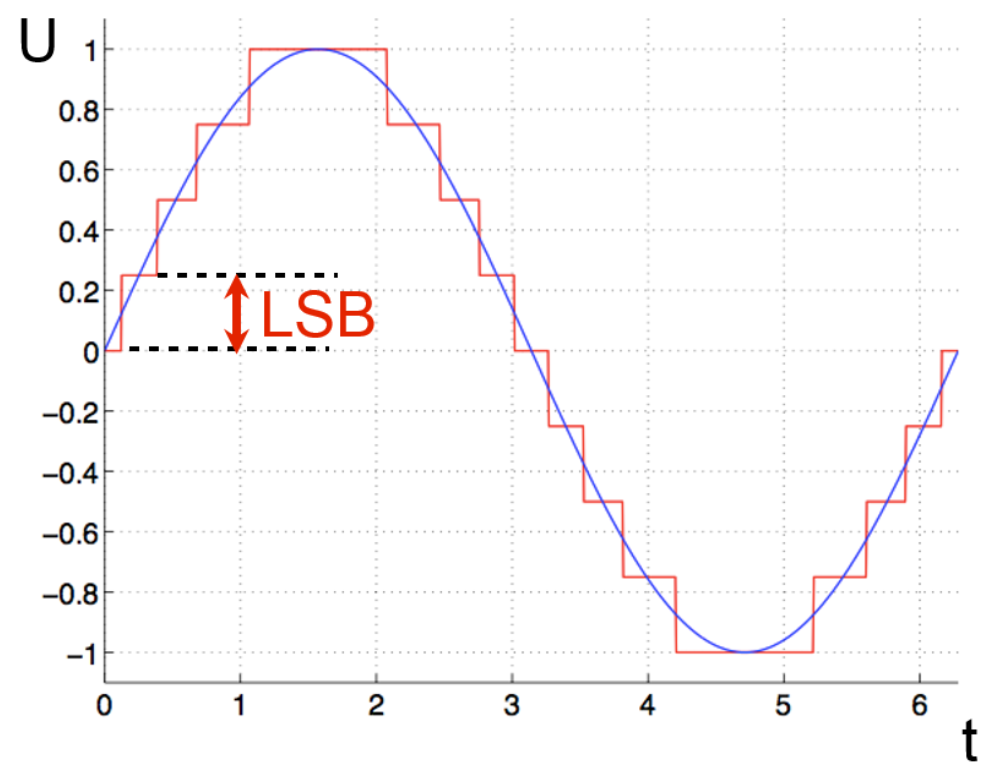
\includegraphics[width=0.5\linewidth]{figs/ad_prevod.png}
    \caption{Vstup a výstup A/D převodníku.}
    \label{fig:vstup-a-vystup-a-d-prevodniku}
\end{figure}
\end{tcolorbox}

\begin{examplebox}[title={Kvantování – příklad}]
\textbf{Otázka:} Jaká je velikost LSB u 8bitového A/D převodníku s rozsahem 0–5 V a jaké digitální slovo odpovídá napětí 0{,}84 V?\\
\textbf{Odpověď:} $U_{LSB} = \frac{5}{2^8} = 0.0195\ V$, $D = 43 = 0010\ 1011$
\end{examplebox}

\begin{tcolorbox}[title={\stepcounter{questionnumber}\thequestionnumber. Jak zní vzorkovací teorém? Jakou vzorkovací frekvenci je rozumné vzorkovat obdélníkový průběh o frekvenci 2 MHz (zdůvodněte proč). (12)}]
\textbf{Vzorkovací teorém:} $f_s > 2 f_{\max}$.\\
\textbf{Obdélník 2 MHz:} obsahuje liché harmonické $3f, 5f, 7f...$ $\Rightarrow$ nestačí jen $2\cdot2$ MHz.

\textbf{Rozumně:} zachytit aspoň několik harmonických, např. do $5f = 10$ MHz $\Rightarrow$ $f_s > 20$ MHz.\\
\textbf{Prakticky:} cca $20$--$50$ MHz podle požadované věrnosti hran.
\end{tcolorbox}

\begin{tcolorbox}[title={\stepcounter{questionnumber}\thequestionnumber. Jak se dá rekonstruovat navzorkovaný signál například pro jeho zobrazení na osciloskopu? Jsou tam nějaké problémy? (18–24)}]
\textbf{Rekonstrukce:} ideální dolní propust / sinc filtr.\\
\textbf{Princip:} každý vzorek se rozprostře funkcí sinc, jejich součet tvoří spojitý průběh.\\
\textbf{Problémy:} ideální filtr je nerealizovatelný, počítá se jen konečný počet vzorků, při porušení $f_s > 2f_{\max}$ vzniká aliasing.
\[x(t) = \sum_{n=-\infty}^{\infty} x[n] \cdot \text{sinc}\left(\frac{t - nT}{T}\right)\]
\end{tcolorbox}

\begin{addonbox}[title={Jaké znáte D/A převodníky? Uveďte u každého typickou oblast použití.}]
\textbf{R-2R síť} - univerzální napěťové DAC, měřicí technika, generátory.\\
\textbf{R-R-R / vážené odpory} - jednoduchý princip, malé rozlišení, výuka / jednoduché DAC.\\
\textbf{Spínané kondenzátory} - integrované DAC/ADC, CMOS, nízká spotřeba.\\
\textbf{PWM + filtr} - mikrokontroléry, levné řízení, audio s menšími nároky.\\
\textbf{$\Delta-\Sigma$ DAC} - audio, vysoké rozlišení, digitální modulátor + analogový filtr.\\
\textbf{Spínané zdroje proudu} - rychlé a přesné DAC, komunikace, RF, video.
\end{addonbox}

\begin{addonbox}[title={Vysvětlete princip funkce D/A převodníku s R-R-R strukturou.}]
\textbf{Princip:} odporový dělič / síť s více odpory vytváří napěťové úrovně odpovídající digitálnímu slovu.\\
\textbf{Bity:} spínače podle kódu připojují uzly na $U_{REF}$ nebo GND.\\
\textbf{Výstup:} vznikne analogové napětí jako podíl z $U_{REF}$.\\
\textbf{Nevýhoda:} pro vyšší rozlišení je potřeba přesnost mnoha odporů a struktura roste hůř než R-2R.\\
\textbf{Použití:} jednoduché / výukové DAC, malé rozlišení.

\begin{figure}[H]
    \centering
    \IfFileExists{figs/dac_rrr_princip.png}
      {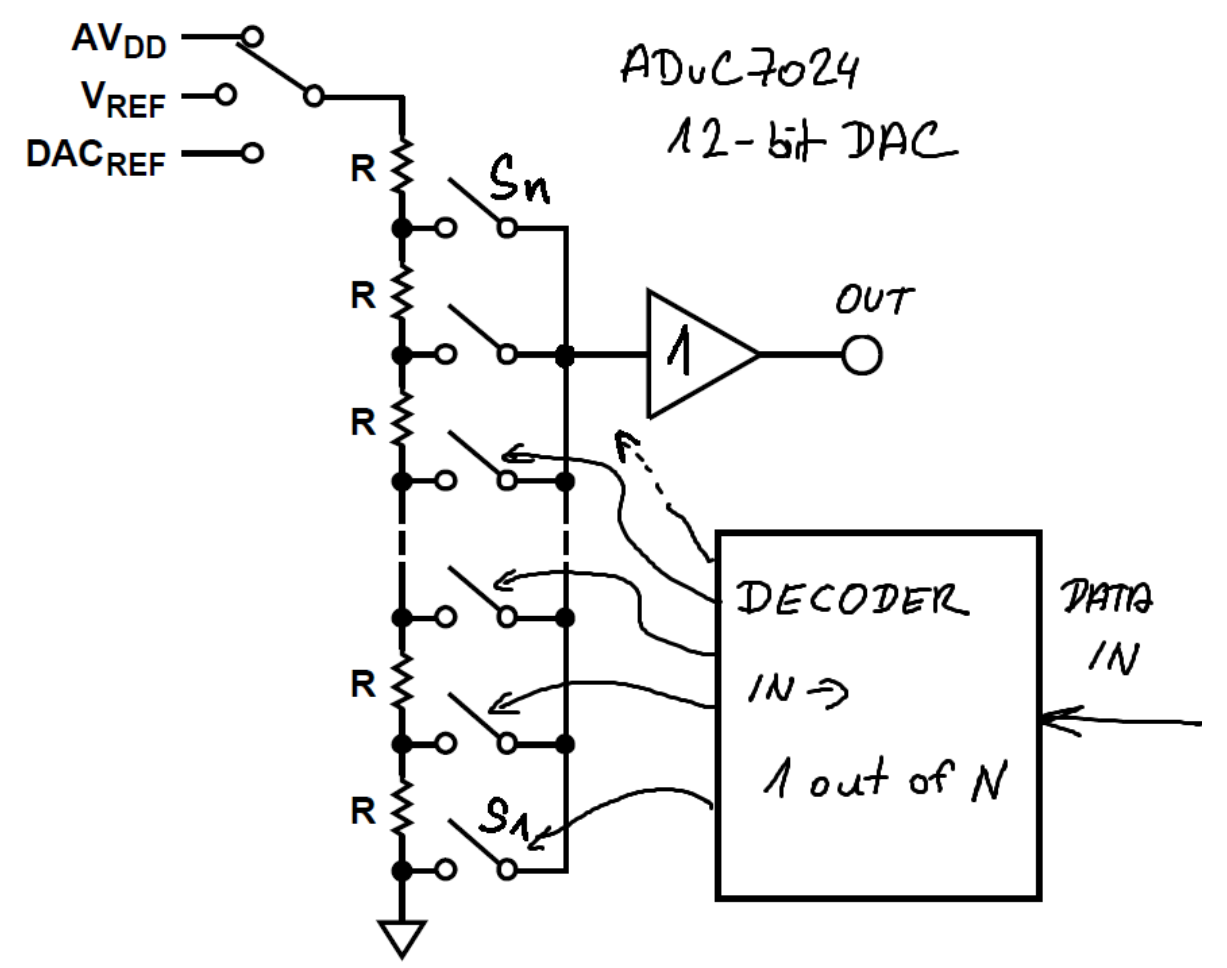
\includegraphics[width=0.55\linewidth]{figs/dac_rrr_princip.png}}
      {\fbox{\parbox{0.55\linewidth}{\centering Chybí obrázek: \texttt{figs/dac\_rrr\_princip.png}}}}
    \caption{Princip D/A převodníku s R-R-R strukturou.}
    \label{fig:dac-rrr-princip}
\end{figure}
\end{addonbox}

\begin{addonbox}[title={Vysvětlete princip funkce D/A převodníku s R-2R sítí.}]
\textbf{Princip:} odporová síť používá jen dvě hodnoty odporu: $R$ a $2R$.\\
\textbf{Bity:} každý bit přepíná svou větev na $U_{REF}$ nebo GND.\\
\textbf{Váhy:} síť zajistí binární vážení proudů/napětí: MSB má váhu $1/2$, další $1/4$, další $1/8$...\\
\textbf{Výstup:} součet vážených příspěvků bitů $\Rightarrow$ analogové napětí úměrné digitálnímu slovu.\\
\textbf{Výhoda:} stačí přesně vyrábět jen poměr $R:2R$, ne mnoho různých odporů.

\begin{figure}[H]
    \centering
    \IfFileExists{figs/dac_r2r_princip.png}
      {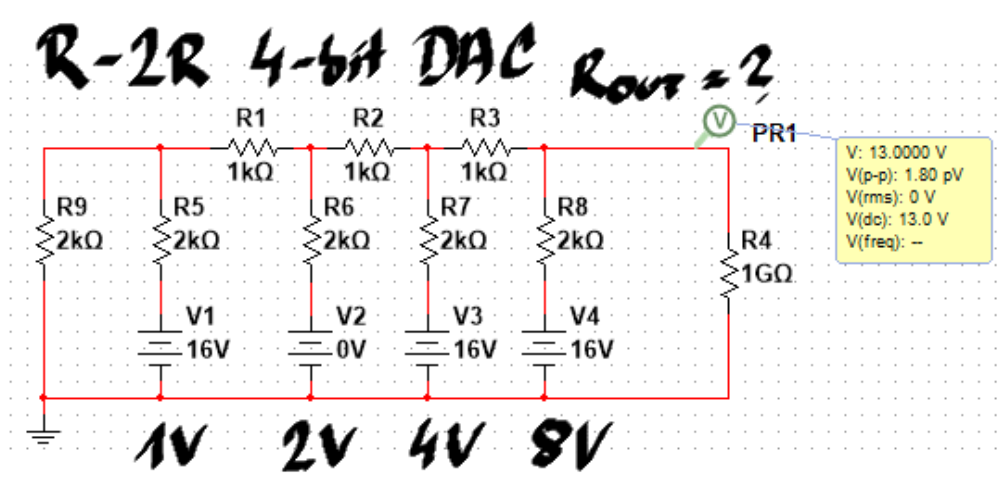
\includegraphics[width=0.55\linewidth]{figs/dac_r2r_princip.png}}
      {\fbox{\parbox{0.55\linewidth}{\centering Chybí obrázek: \texttt{figs/dac\_r2r\_princip.png}}}}
    \caption{Princip D/A převodníku s R-2R sítí.}
    \label{fig:dac-r2r-princip}
\end{figure}
\end{addonbox}


\begin{tcolorbox}[title={\stepcounter{questionnumber}\thequestionnumber. Nakreslete dvoubitový DAC s R-2R strukturou. Zobrazte pro stav MSB 1, LSB 0 a určete výstupní napětí. (29)}]
\begin{figure}[H]
    \centering
    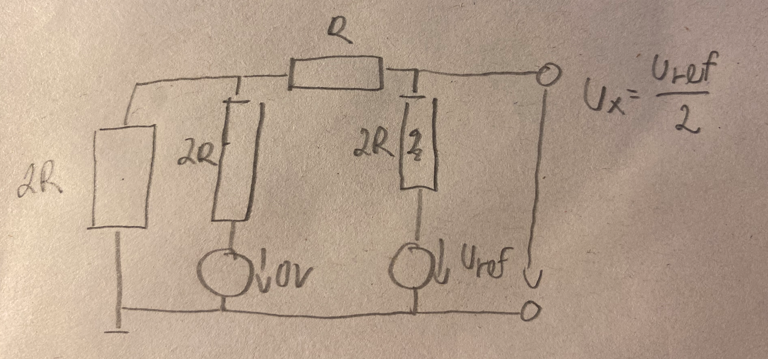
\includegraphics[width=0.5\linewidth]{figs/r2r.png}
    \caption{Dvoubitový DAC s R-2R.}
    \label{fig:dvoubitovy-dac-s-r-2r}
\end{figure}
\end{tcolorbox}




\begin{tcolorbox}[title={\stepcounter{questionnumber}\thequestionnumber. Vysvětlete princip funkce DA převodníku se spínanými kondenzátory (obrázek+příklad, stačí velmi jednoduše..). (31)}]
\textbf{Princip:} kapacitní dělič / přerozdělení náboje.\\
\textbf{1. fáze:} reset, kondenzátory se vybijí.\\
\textbf{2. fáze:} podle bitů se kondenzátory připojí na $U_{REF}$ nebo GND $\Rightarrow$ výsledné napětí odpovídá digitálnímu slovu.\\
\[U_{out} = U_{REF} \cdot \frac{C_{\text{na referenci}}}{C_{total}}\]
\begin{figure}[H]
    \centering
    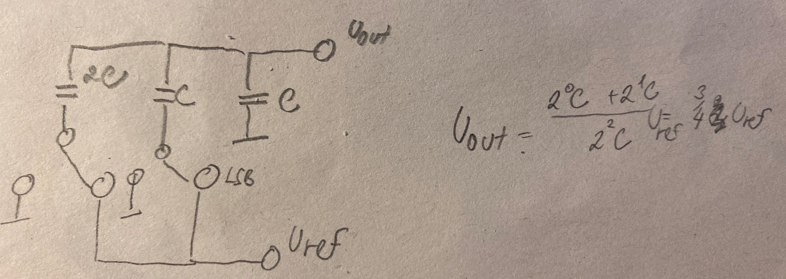
\includegraphics[width=0.5\linewidth]{figs/spinankond.png}
    \caption{DAC s spínanými kondenzátory.}
    \label{fig:dac-s-spinanymi-kondenzatory}
\end{figure}
\end{tcolorbox}

\begin{tcolorbox}[title={\stepcounter{questionnumber}\thequestionnumber. Jaké znáte A/D převodníky? Uveďte u každého typickou oblast použití. (33–46)}]
\textbf{Flash (paralelní)} - nejrychlejší, osciloskopy, radary.\\
\textbf{SAR (postupná aproximace)} - mikroprocesory, běžná měření.\\
\textbf{Dvousklonný integrační} - přesné, pomalé DMM/voltmetry.\\
\textbf{$\Delta-\Sigma$} - vysoké rozlišení, audio, senzory, přesná nízkofrekvenční měření.\\
\textbf{Pipelined} - 2G, 3G, 4G síťové prvky.
\end{tcolorbox}

\begin{tcolorbox}[title={\stepcounter{questionnumber}\thequestionnumber. Jak vzniká kvantizační šum (obrázek)? Jeho hodnota roste nebo klesá s počtem bitů AD převodníku a proč? (35)}]

\textbf{Kvantizační chyba/šum:} rozdíl mezi skutečnou analogovou hodnotou a zaokrouhlenou digitální úrovní.\\
\textbf{LSB:} $q = \frac{\text{rozsah}}{2^N}$, chyba cca $\pm \frac{1}{2}$ LSB.\\
\textbf{S počtem bitů klesá} => více diskrétních úrovní ($2^n$)\\
\begin{figure}[H]
    \centering
    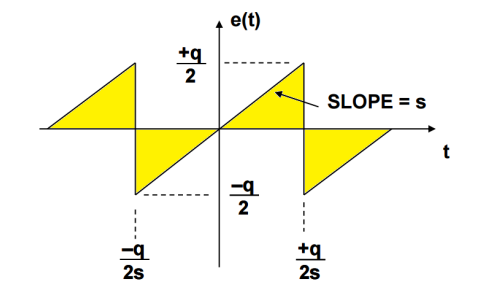
\includegraphics[width=0.5\linewidth]{figs/kvantsum.png}
    \caption{Kvantizační šum.}
    \label{fig:kvantizacni-sum}
\end{figure}
\end{tcolorbox}

\begin{tcolorbox}[title={\stepcounter{questionnumber}\thequestionnumber. Jaký AD převodník se používá v (rychlých) osciloskopech - blokový diagram, kolik komparátorů bude obsahovat 8 bitový převodník? Může se během převodu měnit napětí na vstupu? (38)}]
\textbf{Typ:} flash/paralelní ADC $\Rightarrow$ nejrychlejší.\\
\textbf{Počet komparátorů:} $2^N - 1$, pro 8 bitů: $2^8 - 1 = 255$.\\
\textbf{Vstup:} může se měnit, protože převod probíhá prakticky okamžitě, ale musí být definovaný v okamžiku vzorkování/apertury.
\begin{figure}[H]
    \centering
    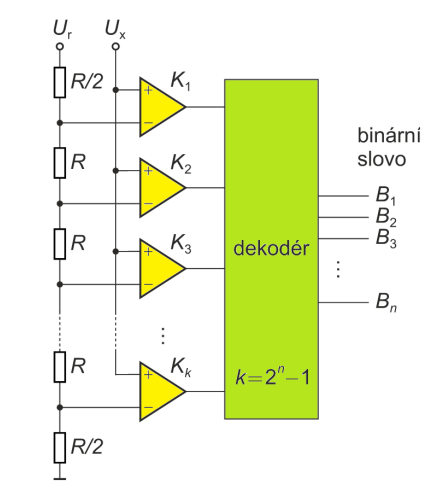
\includegraphics[width=0.4\linewidth]{figs/flash.png}
    \caption{Flash ADC.}
    \label{fig:flash-adc}
\end{figure}
\end{tcolorbox}
\begin{tcolorbox}[title={\stepcounter{questionnumber}\thequestionnumber. Popište princip funkce převodníku s postupnou aproximací (blokový diagram + vysvětlete na nějakém konkrétním příkladě $V_{ref}, V_{in}$). Může se během převodu měnit napětí na vstupu? (39–40)}]

\textbf{Princip:} binární vyhledávání. SAR nastavuje bity od MSB, DAC vytvoří $U_{DAC}$, komparátor porovná $U_{in}$ a $U_{DAC}$.\\
\textbf{Příklad:} rozsah $0$--$10$ V, $U_{in}=7$ V.\\
MSB=1 $\Rightarrow U_{DAC}=5$ V, $7>5$ $\Rightarrow$ bit zůstane 1.\\
Další bit=1 $\Rightarrow U_{DAC}=7{,}5$ V, $7<7{,}5$ $\Rightarrow$ bit se vrátí na 0. Dále stejně pro nižší bity.\\
\textbf{Vstup:} během převodu se nesmí měnit, drží ho vzorkovací \textbf{S\&H obvod}.
\begin{figure}[H]
    \centering
    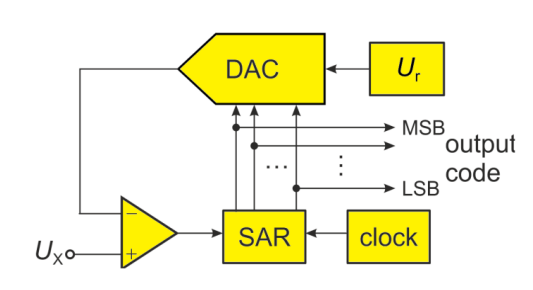
\includegraphics[width=0.4\linewidth]{figs/aproximacni.png}
    \caption{ADC s postupnou aproximací.}
    \label{fig:adc-s-postupnou-aproximaci}
\end{figure}
\end{tcolorbox}

\begin{tcolorbox}[title={\stepcounter{questionnumber}\thequestionnumber. Jaký AD převodník typicky najdete v jednočipových mikrokontrolérech, po kolika krocích získáme výsledek u takovéhoto 16 bitového převodníku? Popište heslovitě princip funkce? (39–40)}]
\textbf{Typicky:} SAR ADC = převodník s postupnou aproximací.\\
\textbf{16 bitů:} výsledek po 16 porovnáních/krocích (+ režie pro vzorkování a uložení dat).\\
\textbf{Princip:} viz předchozí otázka.
\end{tcolorbox}

\begin{tcolorbox}[title={\stepcounter{questionnumber}\thequestionnumber. Popište princip funkce AD převodníku s dvousklonnou integrací (blokový diagram + vysvětlete na nějakém konkrétním příkladě - průběhy pro konkrétní $V_{ref}, V_{in1}, V_{in2}$). Může se během převodu měnit napětí na vstupu? (42–43)}]
\textbf{1. fáze:} integrace neznámého napětí $U_x$ po konstantní dobu $T_1$ (často násobek 20 ms $\Rightarrow$ potlačení 50 Hz).\\
\textbf{2. fáze:} integrace referenčního napětí opačné polarity $U_r$ až do návratu na nulu. Měří se doba $T_2$.\\
\textbf{Vztah:} $U_xT_1 = U_rT_2$ $\Rightarrow$ $U_x = U_r\frac{T_2}{T_1}=U_r\frac{N_2}{N_1}$, kde $N_{1,2}$ jsou počty pulsů.\\
\textbf{Vstup:} měří se střední hodnota během $T_1$; pro DC má být vstup během převodu stabilní. Integrace potlačí periodické rušení, ne libovolné rychlé změny.
\begin{figure}[H]
    \centering
    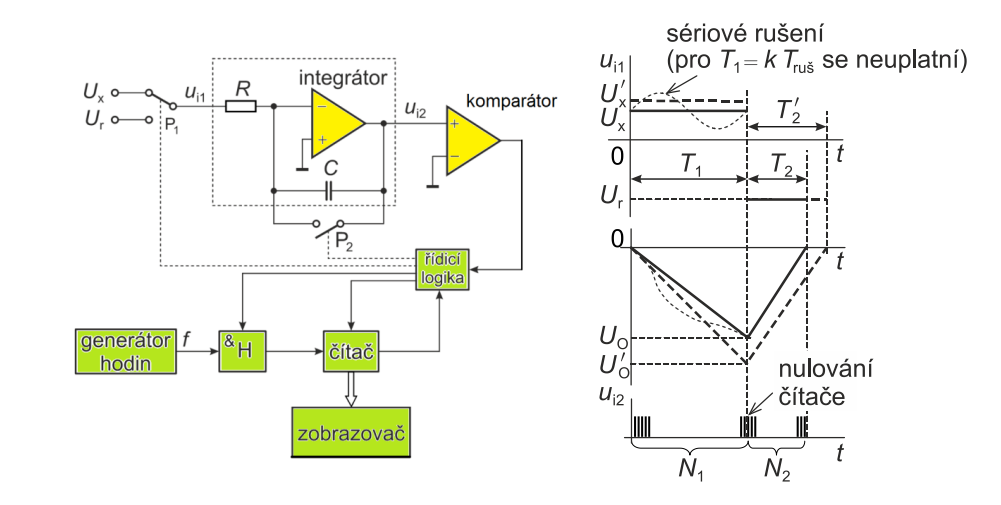
\includegraphics[width=0.6\linewidth]{figs/integracni.png}
    \caption{ADC s dvousklonnou integrací.}
    \label{fig:adc-s-dvousklonnou-integraci}
\end{figure}
\end{tcolorbox}

\begin{tcolorbox}[title={\stepcounter{questionnumber}\thequestionnumber. Popište princip AD převodníku $\Delta\Sigma$ (blokový diagram + tři nejdůležitější principy které používá pro svou činnost). Může se během převodu měnit napětí na vstupu? (44–46)}]
\textbf{Princip:} modulátor vytváří rychlý 1bitový bitstream, jehož střední hodnota odpovídá $U_{in}$. Digitální filtr + decimace z něj udělá výsledné slovo.

\textbf{3 důležité principy:}
\begin{enumerate}
    \item \textbf{Vyrovnávání náboje} - 1bit DAC ve zpětné vazbě kompenzuje vstupní náboj.
    \item \textbf{Převzorkování} - vysoké $f_s$, šum se rozloží do širšího pásma.
    \item \textbf{Tvarování šumu} - kvantizační šum se přesune do vyšších kmitočtů a odstraní se digitálním LPF.
\end{enumerate}

\textbf{Vstup:} může se měnit pomalu; převodník má latenci kvůli digitálnímu filtru.
\begin{figure}[H]
    \centering
    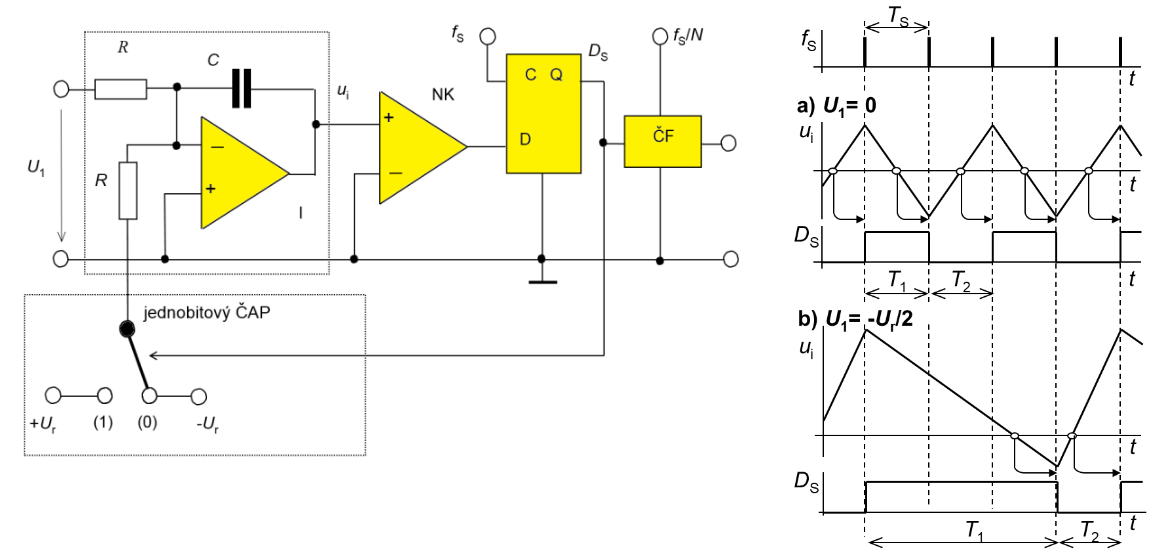
\includegraphics[width=0.8\linewidth]{figs/deltasigmaadc.png}
    \caption{AD převodník $\Delta - \Sigma$.}
    \label{fig:ad-prevodnik-delta-sigma}
\end{figure}
\end{tcolorbox}


\begin{tcolorbox}[title={\stepcounter{questionnumber}\thequestionnumber. Jaké má digitální osciloskop výhody oproti analogovému? (53)}]
\textbf{Jednorázové děje} - umí uložit průběh do paměti.\\
\textbf{Pre-trigger} - vidím i děj před spouštěcí událostí.\\
\textbf{Zpracování dat} - kurzory, automatická měření, FFT, ukládání průběhů.\\
\textbf{Komunikace} - USB/Ethernet, vzdálené ovládání.\\
\textbf{Pokročilý trigger} - hledání vzácných poruch, dekódování sběrnic.
\end{tcolorbox}

\begin{tcolorbox}[title={\stepcounter{questionnumber}\thequestionnumber. Z jakých základních bloků se skládá digitální osciloskop? (55)}]
\textbf{Bloky:} vstupní dělič/zesilovač, anti-alias filtr, ADC, paměť, časová základna, trigger, FPGA/DSP/CPU, displej a ovládání.
\begin{figure}[H]
    \centering
    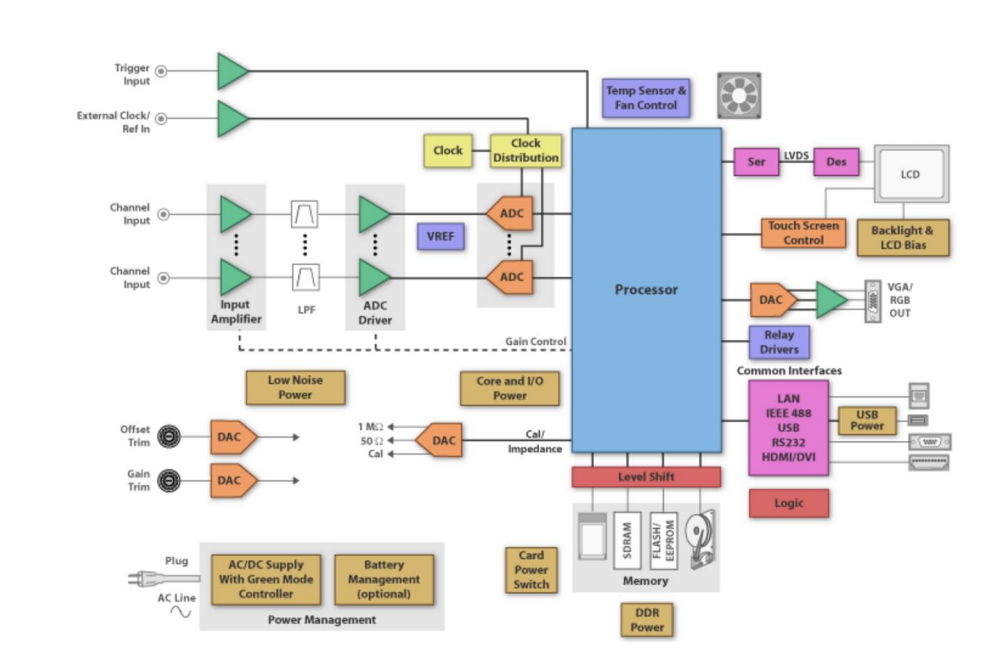
\includegraphics[width=0.8\linewidth]{figs/osciloskopdig.png}
    \caption{Bloky digitálního osciloskopu.}
    \label{fig:bloky-digitalniho-osciloskopu}
\end{figure}
\end{tcolorbox}

\begin{addonbox}[title={Jaké znáte režimy sběru dat u digitálního osciloskopu?}]
\textbf{Normal/sample} - ukládá běžné vzorky podle časové základny.\\
\textbf{Peak detect} - zachytí krátké pulzy/glitche mezi běžnými vzorky.\\
\textbf{Average} - průměrování více průběhů $\Rightarrow$ potlačení náhodného šumu, jen pro opakované děje.\\
\textbf{High resolution} - digitální průměrování/decimace sousedních vzorků $\Rightarrow$ vyšší efektivní rozlišení, menší šířka pásma.\\
\textbf{Envelope} - obálka min/max z více průběhů $\Rightarrow$ vidím rozptyl, rušení, kolísání signálu.
\end{addonbox}

\begin{tcolorbox}[title={\stepcounter{questionnumber}\thequestionnumber. Kdy mohu v osciloskopu použít vzorkování v ekvivalentním čase a proč, co to znamená? (57)}]
\textbf{Použití:} jen pro periodický a stabilní signál.\\
\textbf{Princip:} osciloskop bere vzorky z mnoha period s malým časovým posunem $\Rightarrow$ složí jeden průběh.\\
\textbf{Výhoda:} umožňuje navzorkovat rychlejší signály.\\
\end{tcolorbox}

\begin{tcolorbox}[title={\stepcounter{questionnumber}\thequestionnumber. K čemu slouží funkce TRIGGER u osciloskopu nebo logického analyzátoru? Jaké znáte druhy triggeru - k čemu jsou užitečné? (61, 73)}]
\textbf{Trigger:} spustí/zastaví záznam při definované události $\Rightarrow$ stabilní zobrazení a zachycení poruchy.\\
\textbf{Hranový} - náběžná/sestupná hrana, základní režim.\\
\textbf{Šířka pulzu} - zachycení příliš krátkého/dlouhého pulzu.\\
\textbf{Logický / slovo} - kombinace stavů na více kanálech.\\
\textbf{Sekvence/glitch} - hledání vzácných chyb.

\end{tcolorbox}

\begin{tcolorbox}[title={\stepcounter{questionnumber}\thequestionnumber. Popište princip funkce osciloskopické sondy 10:1, jaké parametry se u sondy řeší a který se kdy uplatní? (62)}]
\textbf{Sonda 10:1:} napěťový dělič, na osciloskop jde $1/10$ napětí.\\
\textbf{Výhoda:} větší vstupní odpor cca $10\,\mathrm{M}\Omega$, menší kapacitní zatížení cca jednotky až desítky pF.\\
\textbf{Odpor:} důležitý pro DC a nízké frekvence.\\
\textbf{Kapacita:} důležitá pro rychlé hrany / vysoké frekvence.\\
\textbf{Kompenzace:} kapacitní dělič musí být nastavený, jinak zkreslí hrany.
\begin{figure}[H]
    \centering
    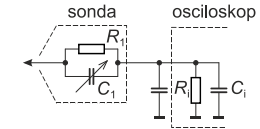
\includegraphics[width=0.3\linewidth]{figs/oscsonda.png}
    \caption{Pasivní sonda 1:10.}
    \label{fig:pasivni-sonda-1-10}
\end{figure}
\end{tcolorbox}

\begin{tcolorbox}[title={\stepcounter{questionnumber}\thequestionnumber. K čemu slouží osciloskopická sonda (náhradní zapojení, funkce)? U vstupu osciloskopu můžete najít údaj 1M$\Omega$, 25pF - pro jaké měření je který údaj důležitý? (62)}]
Viz předchozí otázka.\\
\textbf{$1\,\mathrm{M}\Omega$:} zatížení pro DC / nízké frekvence.\\
\textbf{25 pF:} kapacitní zatížení pro rychlé hrany / vysoké frekvence.
\end{tcolorbox}

\begin{tcolorbox}[title={\stepcounter{questionnumber}\thequestionnumber. Nakreslete blokový diagram logického analyzátoru, jaké parametry byste očekávali ve specifikaci log. analyzátoru? (68, 75)}]
\textbf{Parametry:} max. vzorkovací frekvence, počet kanálů, rozhodovací úroveň, paměť na kanál, vstupní impedance sondy.\\
\textbf{Režimy:} časová analýza, stavová analýza, glitch/transitional timing.
\begin{figure}[H]
    \centering
    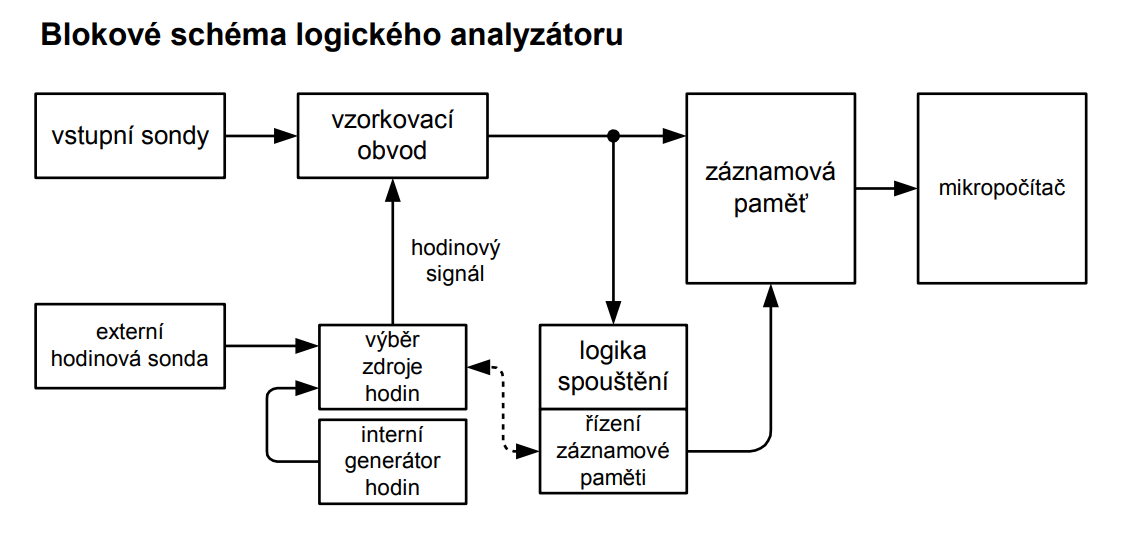
\includegraphics[width=0.6\linewidth]{figs/logicky_analyzator_blokove_schema.png}
    \caption{Blokové schéma logického analyzátoru.}
    \label{fig:blokove-schema-logickeho-analyzatoru}
\end{figure}
\end{tcolorbox}

\begin{tcolorbox}[title={\stepcounter{questionnumber}\thequestionnumber. Jaký je rozdíl mezi asynchronní a synchronní analýzou u logického analyzátoru. Je některá výhodnější například pro interpretaci naměřených dat? (69–72)}]
\textbf{Asynchronní / časová:} interní hodiny, ekvidistantní vzorky $\Rightarrow$ dobré pro časové průběhy a hledání glitchů.\\
\textbf{Synchronní / stavová:} externí hodiny z měřeného zařízení $\Rightarrow$ vzorkuje se v okamžicích platnosti dat.\\
\textbf{Interpretace dat:} synchronní bývá lepší pro sběrnice/stavy zařízení, protože data jsou vztažená k hodinám systému.
\end{tcolorbox}


% ---------------------------------------------------------
% 2 — Měření napětí, proudu, kmitočtu
% ---------------------------------------------------------

\newpage
\section*{2. Měření napětí, proudu a kmitočtu, čítač, měření fáze, chyby a nejistoty}
\setcounter{chapternumber}{2}
\setcounter{questionnumber}{0}
% ---------------------------------------------------------

\begin{tcolorbox}[title={\stepcounter{questionnumber}\thequestionnumber. Jaký vnitřní (vstupní resp. výstupní) odpor má ideální: voltmetr, ampérmetr, zdroj napětí, zdroj proudu, převodník I/U s OZ? (2)}]
\textbf{Voltmetr:} $R_{in}\to\infty$ -- měří napětí paralelně a nemá zatěžovat obvod.\\
\textbf{Ampérmetr:} $R_{in}\to0$ -- měří proud sériově a nemá způsobit úbytek napětí.\\
\textbf{Ideální zdroj napětí:} $R_{out}\to0$ -- drží napětí i při změně zátěže.\\
\textbf{Ideální zdroj proudu:} $R_{out}\to\infty$ -- drží proud i při změně zátěže.\\
\textbf{Převodník I/U s OZ:} vstup je ve virtuální zemi, tedy $R_{in}\approx0$; výstup OZ má $R_{out}\approx0$.
\end{tcolorbox}

\begin{tcolorbox}[title={\stepcounter{questionnumber}\thequestionnumber. Jaké základní bloky najdete v DMM, který měří ACV, DCV, ACI, DCI, R? (3–4)}]
\begin{figure}[H]
    \centering
    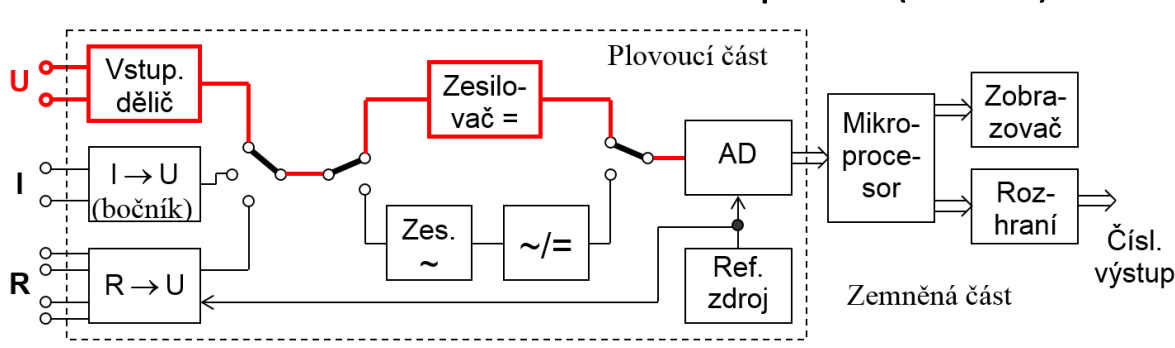
\includegraphics[width=0.8\linewidth]{figs/blokydmm.png}
    \caption{Základní bloky DMM.}
    \label{fig:zakladni-bloky-dmm}
\end{figure}
\end{tcolorbox}

\begin{tcolorbox}[title={\stepcounter{questionnumber}\thequestionnumber. Nakreslete princip (schéma), jakým se v číslicovém multimetru přepínají rozsahy při měření stejnosměrného napětí (včetně uvedení hodnot U, I, R). (4–5)}]
\textbf{Typická hodnota:} $R_{in}=10~\mathrm{M\Omega}$, aby voltmetr měřený obvod zatěžoval co nejméně.\\
\begin{figure}[H]
    \centering
    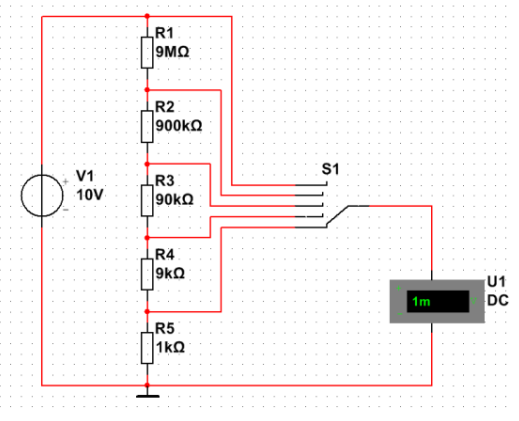
\includegraphics[width=0.5\linewidth]{figs/vstupni_napetovy_delic_voltmetr.png}
    \caption{Vstupní napěťový dělič pro voltmetr.}
    \label{fig:vstupni-napetovy-delic-pro-voltmetr}
\end{figure}
\end{tcolorbox}

\begin{examplebox}[title={Multimetr – návrh vstupního děliče}]
\textbf{Zadání:} Navrhněte více-rozsahový vstupní dělič digitálního voltmetru s celkovým vstupním odporem 10~M$\Omega$ pro rozsah 0--10~V.\\
\textbf{Postup:} zvolí se proud děličem, celkový odpor zůstane 10~M$\Omega$ a odbočky se nastaví tak, aby na vstupu A/D převodníku bylo při plném rozsahu jeho jmenovité napětí.\\
\textbf{Schéma:} viz obrázek vstupního děliče výše.
\end{examplebox}

\begin{tcolorbox}[title={\stepcounter{questionnumber}\thequestionnumber. Proč je výhodné čtyř-svorkové připojení proudového bočníku, například v multimetru, nakreslete zapojení. (7)}]
\textbf{Problém:} odpor vodičů a přechodů způsobuje chybu.\\
\textbf{Řešení:} proud teče dvěma proudovými svorkami, ale napětí se měří samostatnými napěťovými svorkami přímo na bočníku.\\
\begin{figure}[H]
    \centering
    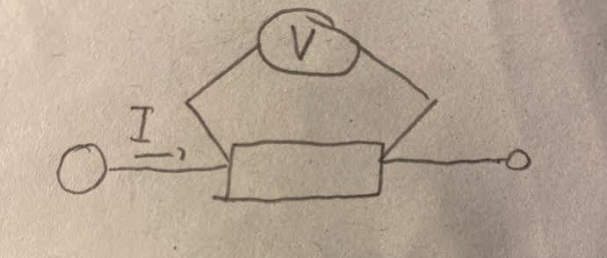
\includegraphics[width=0.5\linewidth]{figs/bocnik.png}
    \caption{Čtyřsvorkové zapojení.}
    \label{fig:ctyrsvorkove-zapojeni}
\end{figure}
\end{tcolorbox}

\begin{tcolorbox}[title={\stepcounter{questionnumber}\thequestionnumber. Nakreslete princip, jakým se v číslicovém multimetru přepínají rozsahy při měření stejnosměrného proudu (včetně vedení hodnot U, I, R). (8)}]
\textbf{Princip:} proud se převádí na napětí pomocí \textbf{bočníku}: $U_B=I\,R_B$. A/D převodník pak měří úbytek na bočníku.\\
\textbf{Příklad rozsahů:} $I_3=10~A$, $I_2=1~A$, $I_1=0{,}1~A$.\\
\textbf{Příklad odporů:} $R_3=0{,}1~\Omega$, $R_2=0{,}9~\Omega$, $R_1=9~\Omega$.\\
\begin{figure}[H]
    \centering
    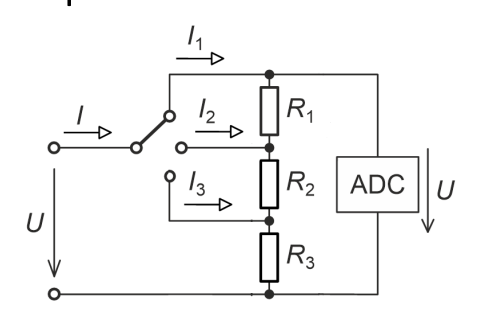
\includegraphics[width=0.5\linewidth]{figs/ayrtonuv_bocnik.png}
    \caption{Ayrtonův bočník.}
    \label{fig:ayrtonuv-bocnik}
\end{figure}
\end{tcolorbox}

\begin{examplebox}[title={Ampérmetr – změna rozsahu}]
\textbf{Zadání:} Navrhněte síť bočníků pro ampérmetr tak, aby bylo možné přepínat mezi několika proudovými rozsahy.\\
\textbf{Schéma:} viz Ayrtonův bočník výše.
\end{examplebox}

\begin{tcolorbox}[title={\stepcounter{questionnumber}\thequestionnumber. Levný ruční číslicový multimetr měří efektivní hodnotu napětí typicky přes měření střední hodnoty napětí. Jaký obvod použiji, aby se neuplatnila nelineární charakteristika diod při měření malých napětí (např. 2Vrms)? (9–11)}]
\textbf{Levný DMM:} změří střední usměrněnou hodnotu a pro sinus ji přepočte na efektivní hodnotu:
\[U_{ef} \approx 1{,}11\,U_{\mathrm{str,usm}}.\]
Zdroj proudu protlačí proud, i když je napětí malé.
\begin{figure}[H]
    \centering
    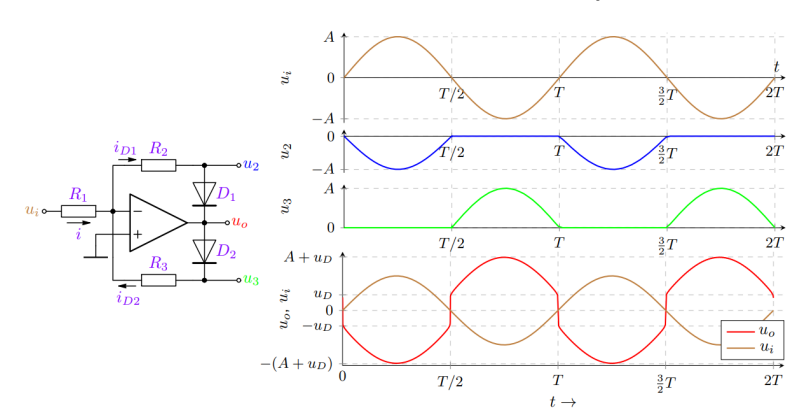
\includegraphics[width=0.5\linewidth]{figs/usmernovac.png}
    \caption{Usměrňovač.}
    \label{fig:usmernovac}
\end{figure}
\end{tcolorbox}

\begin{tcolorbox}[title={\stepcounter{questionnumber}\thequestionnumber. Co to znamená, že vstupní část digitálního multimetru je „plovoucí“ a jak se to v praxi zajistí (alespoň dva způsoby, obrázek)? (15)}]
\textbf{Plovoucí vstup:} měřicí část nemá pevný potenciál vůči zemi. Může tedy měřit i na nenulovém společném potenciálu, pokud nejsou překročeny izolační limity.\\
\textbf{Praktické zajištění:} bateriové napájení, galvanicky oddělený zdroj, optočleny, transformátorový přenos dat, izolační mezery na DPS, guard ring.\\
\begin{figure}[H]
    \centering
    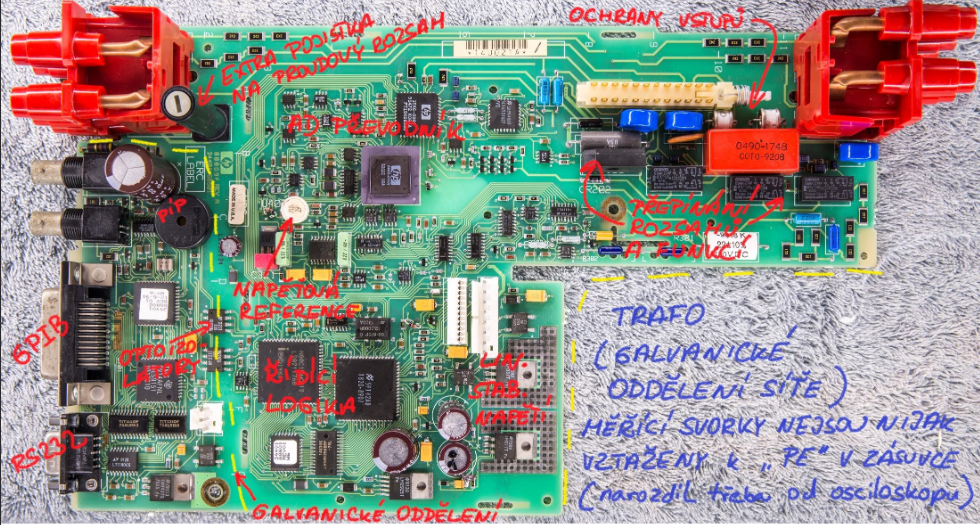
\includegraphics[width=0.75\linewidth]{figs/galvanice_oddeleni.png}
    \caption{Plovoucí vstup.}
    \label{fig:plovouci-vstup}
\end{figure}
\end{tcolorbox}

\begin{tcolorbox}[title={\stepcounter{questionnumber}\thequestionnumber. Nakreslete princip (schéma), jak zjistíte vnitřní odpor multimetru v režimu voltmetr (včetně uvedení hodnot U,I,R). (16–17)}]
\textbf{1. varianta:} voltmetr se připojí do děliče se známým odporem. Z poklesu měřeného napětí se dopočítá jeho vstupní odpor.\\
\textbf{2. varianta:}
\begin{figure}[H]
    \centering
    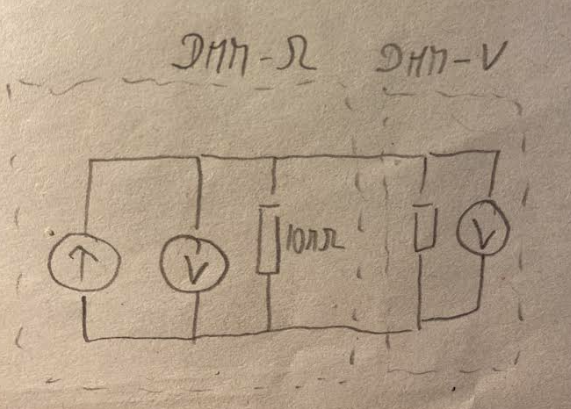
\includegraphics[width=0.5\linewidth]{figs/odpor_voltmetru_schema.png}
    \caption{Schéma měření vn. odporu voltmetru.}
    \label{fig:schema-mereni-vn-odporu-voltmetru}
\end{figure}
\end{tcolorbox}

\begin{tcolorbox}[title={\stepcounter{questionnumber}\thequestionnumber. Nakreslete princip (schéma), jak zjistíte vnitřní odpor multimetru v režimu ampérmetr (včetně uvedení hodnot U,I,R). (18–19)}]
\textbf{1. varianta:} ampérmetr se zapojí paralelně voltmetrr => ohmův zákon.\\
\textbf{2. varianta:}
\begin{figure}[H]
    \centering
    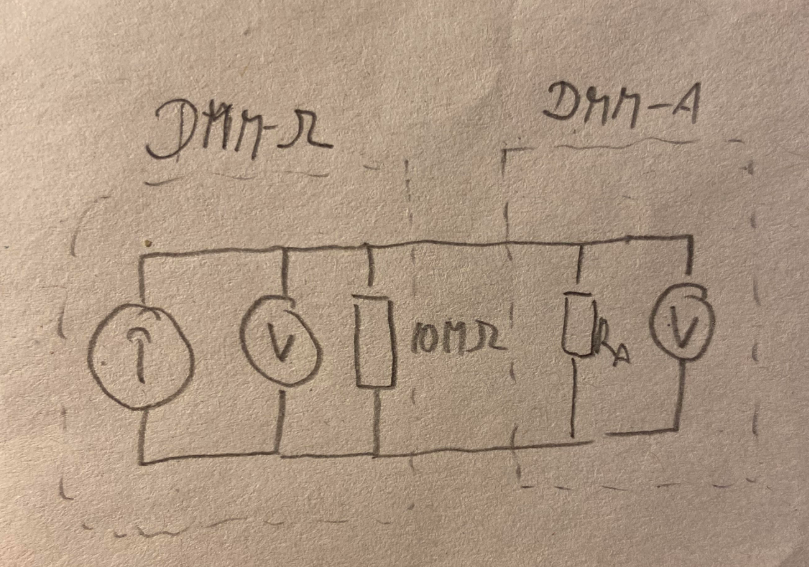
\includegraphics[width=0.5\linewidth]{figs/odpor_ampermetru_schema.png}
    \caption{Schéma měření vn. odporu ampérmetru.}
    \label{fig:schema-mereni-vn-odporu-ampermetru}
\end{figure}
\end{tcolorbox}

\begin{tcolorbox}[title={\stepcounter{questionnumber}\thequestionnumber. Nakreslete princip (schéma), jak zjistíte měřicí proud multimetru v režimu ohmmetr (včetně uvedení hodnot U,I,R). (20)}]
viz předchozí schéma.\end{tcolorbox}

\begin{tcolorbox}[title={\stepcounter{questionnumber}\thequestionnumber. Na jakém principu funguje analogový magnetoelektrický ručičkový voltmetr, z jakého zákona se dá odvodit jeho funkce? (22–23)}]
\textbf{Princip:} Síla působí na proudovodič v mag. poli B, síla otáčí ukazatel.\\
\textbf{Zákon:} Lenzův, vychází z Ampérovy / Lorentzovy síly na vodič s proudem:
\[F=BIl.\]
\begin{figure}[H]
    \centering
    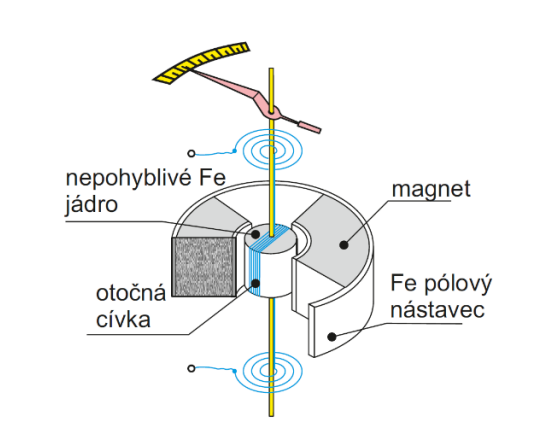
\includegraphics[width=0.5\linewidth]{figs/magnetoel.png}
    \caption{Magnetoel. ručičkový voltmetr.}
    \label{fig:magnetoel-rucickovy-voltmetr}
\end{figure}
\end{tcolorbox}

\begin{tcolorbox}[title={\stepcounter{questionnumber}\thequestionnumber. Popište, jak funguje měření frekvence (signálu s frekvencí f = 10 MHz). (27)}]
\textbf{Pro vysokou frekvenci:} použije se přímé měření frekvence.\\
\textbf{Postup:} vstupní signál se upraví na obdélníkový tvar, otevře se hradlo na přesný čas $T_N$ a čítač spočítá počet period $N$.\\
\textbf{Vztah:}
\[f_x=\frac{N}{T_N}.\]
\begin{figure}[H]
    \centering
    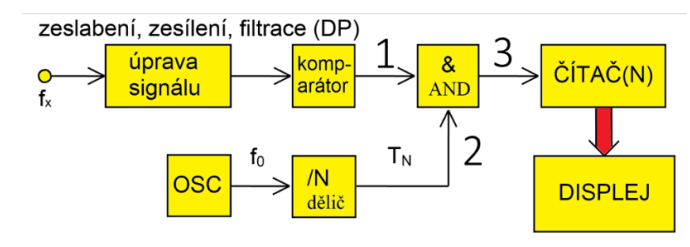
\includegraphics[width=0.5\linewidth]{figs/mereni_frekvence.png}
    \caption{Měření frekvence.}
    \label{fig:mereni-frekvence}
\end{figure}
\end{tcolorbox}

\begin{tcolorbox}[title={\stepcounter{questionnumber}\thequestionnumber. Pokud chci změřit přesnou frekvenci sinusového signálu o frekvenci přibližně 9 MHz, jak to udělám? (schéma) (27)}]
\textbf{Schéma:} viz měření frekvence výše.
\end{tcolorbox}

\begin{tcolorbox}[title={\stepcounter{questionnumber}\thequestionnumber. Popište, jak funguje měření frekvence (periody) signálu s frekvencí f = 1 Hz). (28)}]
\textbf{Pro nízkou frekvenci:} výhodnější je měřit \textbf{periodu}, protože při přímém čítání by za 1~s prošlo jen málo impulsů.\\
\textbf{Postup:} měřený signál otevře hradlo na dobu jedné periody $T_x$ a čítač počítá impulsy časové základny $f_N$.\\
\textbf{Vztah:}
\[T_x=\frac{N}{f_N}, \qquad f_x=\frac{1}{T_x}=\frac{f_N}{N}.\]
\begin{figure}[H]
    \centering
    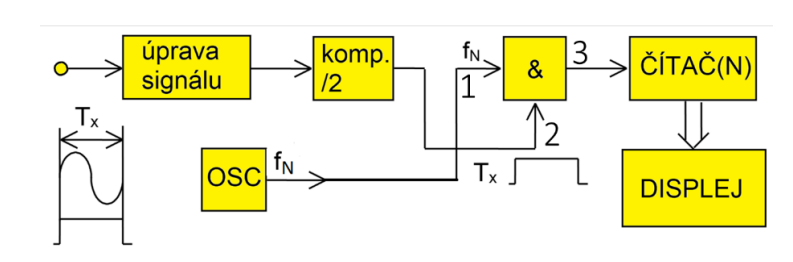
\includegraphics[width=0.5\linewidth]{figs/mereni_periody.png}
    \caption{Měření periody.}
    \label{fig:mereni-periody}
\end{figure}
\end{tcolorbox}

\begin{tcolorbox}[title={\stepcounter{questionnumber}\thequestionnumber. Pokud chci změřit přesnou frekvenci sinusového signálu o frekvenci přibližně 9 Hz, jak to udělám? (schéma) (28)}]
\textbf{Schéma:} viz měření periody výše.
\end{tcolorbox}

\begin{tcolorbox}[title={\stepcounter{questionnumber}\thequestionnumber. Pokud chci přesně změřit frekvenci signálu a neznám předem jeho frekvenci/tvar/amplitudu, jak budu postupovat? A proč (obrázek)? (27–28)}]
\textbf{1. Nejprve osciloskop:} zjistím tvar, amplitudu a přibližná frekvence.\\
\textbf{2. Úprava signálu:} podle amplitudy nastavím komparátor.\\
\textbf{3. Volba metody:} vysoká frekvence $\Rightarrow$ čítání frekvence; nízká frekvence $\Rightarrow$ měření periody.\\
\end{tcolorbox}

\begin{tcolorbox}[title={\stepcounter{questionnumber}\thequestionnumber. Čemu je úměrná hodnota na výstupu synchronního detektoru (například spínačového typu), k čemu se dá synchronní detektor použít. (32–34)}]
\textbf{Princip:} měřený signál se násobí referenčním signálem stejné frekvence a výsledek se filtruje dolní propustí.\\
\textbf{Výstupní DC složka:}
\[U_{out}\sim U_m\cos\varphi, \qquad \omega_r=\omega_1.\]
\textbf{Co zůstane po filtraci:} jen složka signálu, která má stejnou frekvenci a definovaný fázový vztah k referenci.\\
\textbf{Použití:} lock-in zesilovač, měření slabého signálu v šumu, měření amplitudy a fáze odezvy.
\begin{figure}[H]
    \centering
    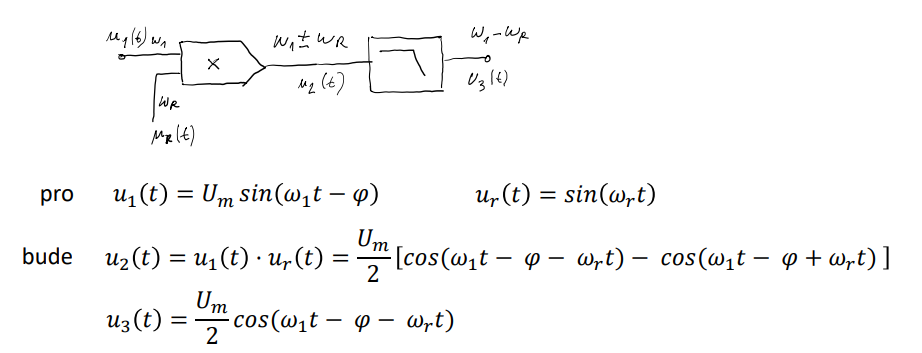
\includegraphics[width=0.5\linewidth]{figs/lockin.png}
    \caption{Synchronní detektor.}
    \label{fig:synchronni-detektor}
\end{figure}
\end{tcolorbox}

\begin{tcolorbox}[title={\stepcounter{questionnumber}\thequestionnumber. Jak se dá změřit změna amplitudy a fáze napětí vůči referenčnímu signálu? Kdy je třeba měřit reálnou a imaginární složku napětí? (31–34)}]
\textbf{Metoda:} použije se \textbf{kvadraturní synchronní detektor} neboli I/Q detekce.\\
\textbf{Dvě reference:} 
\begin{itemize}
    \item Ve fázi $0^\circ$ => $U_{\mathrm{Re}}=U\cos\varphi.$
    \item Posunutá o $90^\circ$ => $U_{\mathrm{Im}}=U\sin\varphi.$
\end{itemize}
\textbf{Amplituda a fáze:}
\[U=\sqrt{U_{\mathrm{Re}}^2+U_{\mathrm{Im}}^2}, \qquad
\varphi=\arctan\left(\frac{U_{\mathrm{Im}}}{U_{\mathrm{Re}}}\right).\]
\textbf{Kdy je to potřeba:} při měření komplexní odezvy, impedance, fázového posuvu, kapacitní/induktivní složky a obecně tam, kde nestačí jen amplituda.
\begin{figure}[H]
    \centering
    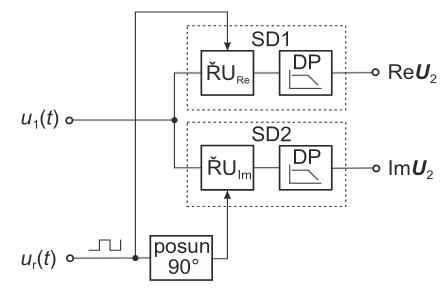
\includegraphics[width=0.5\linewidth]{figs/kvadraturni_synchronni_detektor.png}
    \caption{Kvadraturní synchronní detektor.}
    \label{fig:kvadraturni-synchronni-detektor}
\end{figure}
\end{tcolorbox}

\begin{tcolorbox}[title={\stepcounter{questionnumber}\thequestionnumber. Měřili jsme napětí číslicovým multimetrem. Ten na svém čtyřmístném displeji ukázal hodnotu 10.33 V. Výrobce uvádí chybu měření jako 0.2\% RDG + 3 digity. Napište, jak spočtete nerozšířenou hodnotu nejistoty měření typu B. (44–47)}]
\textbf{Standardní nejistota typu B:}
\[u_U=\frac{\Delta U}{\sqrt{3}}=\frac{\frac{0{,}2}{100}10{,}33+3\cdot0{,}01}{\sqrt{3}}~[V].\]
\end{tcolorbox}

\begin{tcolorbox}[title={\stepcounter{questionnumber}\thequestionnumber. Ohmmetr s pětimístným displejem naměřil odpor 152.03 Ohm. Výrobce uvádí nejistotu pro rozsah 200 Ohm jako: ±0.1\% RDG ± 0.1\% FS. Bude při měření odporu 5.52 Ohm na stejném rozsahu absolutní nejistota měření větší nebo menší? (zdůvodněte). (46–47)}]
\textbf{Pro hodnotu 152{,}03~$\Omega$:}
\[u_R=\frac{\frac{0{,}1}{100}152{,}03+\frac{0{,}1}{100}200}{\sqrt{3}}~[\Omega].\]
\textbf{Pro hodnotu 5{,}52~$\Omega$:} absolutní nejistota bude \textbf{menší}, protože část \textbf{\%RDG} klesne s odečtenou hodnotou.\\
\textbf{Ale pozor:} část \textbf{\%FS} zůstává stejná, protože rozsah 200~$\Omega$ se nezměnil. Relativní nejistota tedy bude u malého odporu horší.
\end{tcolorbox}

\begin{examplebox}[title={Příklad – výpočet nejistoty měření odporu Ohmovou metodou}]
\textbf{Zadání:} Určete standardní a rozšířenou nejistotu měření odporu Ohmovou metodou.
\begin{itemize}
    \item Voltmetr: rozsah 200 mV, přesnost $\pm0{,}1\%$ z odečtené hodnoty a $\pm0{,}05\%$ z rozsahu, naměřeno $U=150~\mathrm{mV}$.
    \item Ampérmetr: rozsah 1{,}2 A, třída přesnosti TP = 0{,}5, naměřeno $I=0{,}4~\mathrm{A}$.
    \item Koeficient rozšíření: $k_r=2$.
\end{itemize}
\textbf{Měřený odpor:}
\[R_x=\frac{U}{I}=\frac{0{,}15}{0{,}4}=0{,}375~\Omega.\]
\textbf{Standardní nejistoty vstupů:}
\[u_U=\frac{\frac{0{,}1}{100}0{,}15+\frac{0{,}05}{100}0{,}2}{\sqrt{3}}=0{,}144~\mathrm{mV},\]
\[u_I=\frac{\frac{0{,}5}{100}1{,}2}{\sqrt{3}}=3{,}46~\mathrm{mA}.\]
\textbf{Přenos nejistot pro $R=U/I$:}
\[u_R=\sqrt{\left(\frac{1}{I}\right)^2u_U^2+\left(-\frac{U}{I^2}\right)^2u_I^2}=3{,}26~\mathrm{m\Omega}.\]
\textbf{Relativní nejistota:} $u_R/R_x=0{,}87~\%$.\\
\textbf{Rozšířená nejistota:} $U_R=k_ru_R=6{,}54~\mathrm{m\Omega}$.
\end{examplebox}

% ---------------------------------------------------------
% 3 — Měření efektivní hodnoty, výkonu a energie
% ---------------------------------------------------------

\newpage\section*{3. Měření efektivní hodnoty, výkonu a spotřeby energie}
\setcounter{chapternumber}{3}
\setcounter{questionnumber}{0}
% ---------------------------------------------------------

\begin{tcolorbox}[title={\stepcounter{questionnumber}\thequestionnumber. Jak je definována efektivní hodnota napětí – vzoreček + definice (přes teplo). (2)}]
\textbf{Definice:} $U_{RMS}$ je hodnota stejnosměrného napětí, která na odporové zátěži vyvolá stejný průměrný výkon / tepelný účinek jako dané střídavé napětí.
\[
U_{RMS}=\sqrt{\frac{1}{T}\int_0^T u^2(t)\,dt}
\]
\end{tcolorbox}

\begin{tcolorbox}[title={\stepcounter{questionnumber}\thequestionnumber. Jakou hodnotu střídavého napětí měří nejlevnější multimetry a jakou preciznější přístroje, jakou zobrazují na displeji? Jak je definována efektivní hodnota napětí, znáte nějakou „analogovou“ metodu výpočtu? (3–5, 10)}]
\textbf{Levné DMM:} měří střední usměrněnou hodnotu $U_{str,usm}$ a pro sinus zobrazí
\[U_{RMS}=1{,}11\,U_{str,usm}\]
=> pro nesinusový průběh chyba podle tvaru signálu.\\
\textbf{True RMS DMM:} měří skutečnou efektivní hodnotu podle definice.\\
\textbf{Analogově:} implicitní RMS převodník, explicitní převodník, tepelný RMS převodník.
\end{tcolorbox}

\begin{tcolorbox}[title={\stepcounter{questionnumber}\thequestionnumber. Na obrázku ukažte jeden princip analogového výpočtu efektivní hodnoty napětí (Explicitní nebo implicitní). (4–5)}]
\textbf{Explicitní:} umocnění $u^2(t)$ => průměrování DP => odmocnění.
\[V_O=\sqrt{\overline{V_{IN}^2}}\]
\begin{figure}[H]
\centering
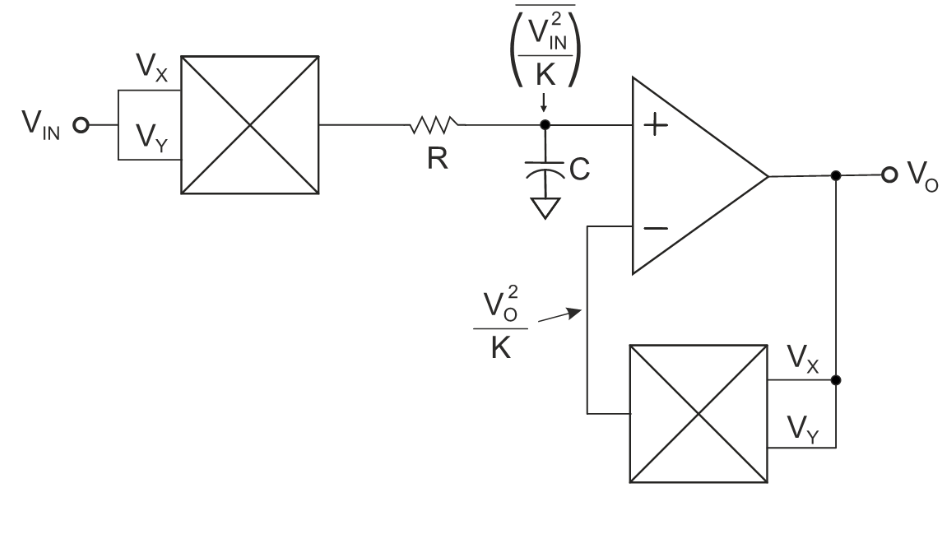
\includegraphics[width=0.55\linewidth]{figs/explicit_rms.png}
\caption{Explicitní analogový převodník RMS.}
\label{fig:explicitni-analogovy-prevodnik-rms}
\end{figure}

\textbf{Implicitní:} ve zpětné vazbě se dělí výstupní hodnotou $U_{10}$:
\[
U_{10}=\frac{1}{T}\int_0^T\frac{u_x^2(t)}{U_{10}}\,dt
\Rightarrow
U_{10}=\sqrt{\frac{1}{T}\int_0^T u_x^2(t)\,dt}
\]
\begin{figure}[H]
\centering
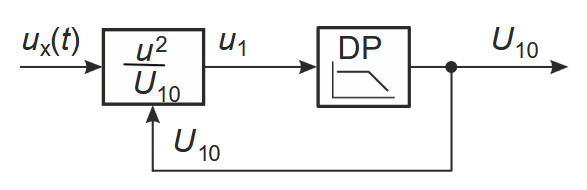
\includegraphics[width=0.5\linewidth]{figs/implicitni_prevodnik.png}
\caption{Implicitní analogový převodník RMS.}
\label{fig:implicitni-analogovy-prevodnik-rms}
\end{figure}
\end{tcolorbox}

\begin{tcolorbox}[title={\stepcounter{questionnumber}\thequestionnumber. Jak funguje převodník pro RMS hodnotu napětí využívající tepelné účinky? (principielní schéma). (7)}]
\textbf{Princip:} tepelný výkon na odporu je úměrný druhé mocnině napětí:
\[P=\frac{u^2}{R}\]
Střídavý vstup ohřívá odpor/tranzistor, teplota se snímá termočlánkem nebo BE přechodem. Zpětná vazba nastaví výstup tak, aby odpovídal stejnému ohřevu => $U_{OUT}=U_{RMS}$.\\
\textbf{Použití:} metrologické přístroje, kalibrátory; přesnost desítky ppm až $0{,}05\%$.
\begin{figure}[H]
    \centering
    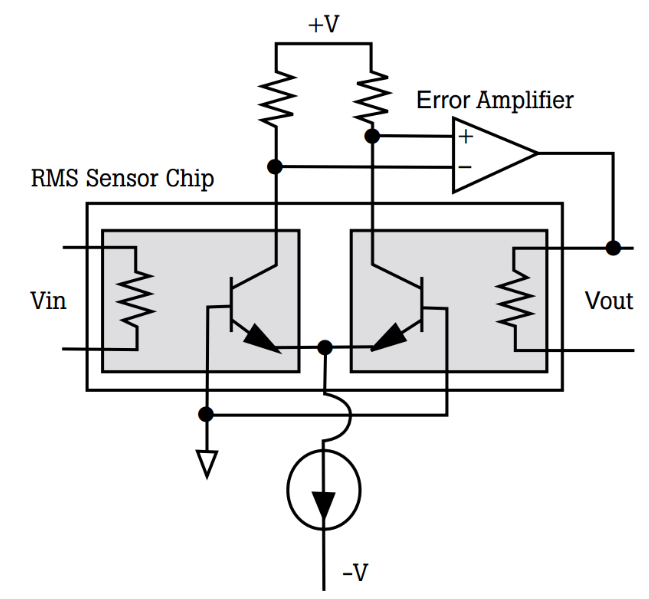
\includegraphics[width=0.4\linewidth]{figs/tepelny_prevodnik_rms.png}
    \caption{Tepelný analogový převodník RMS.}
    \label{fig:tepelny-analogovy-prevodnik-rms}
\end{figure}
\end{tcolorbox}

\begin{tcolorbox}[title={\stepcounter{questionnumber}\thequestionnumber. Jak se měří efektivní hodnota napětí v moderním číslicovém elektroměru? (obrázek s postupem pro asynchronní vzorkování). (8, 9, 20)}]
\textbf{Výpočet ze vzorků:}
\[
U_{RMS}=\sqrt{\frac{1}{N}\sum_{n=1}^{N}u^2[n]}
\]
\textbf{Asynchronní vzorkování:} vzorkuje se nezávisle na přesné periodě sítě; průměrování/integrace se nahradí dolní propustí. Funguje pro obecný periodický průběh při splnění vzorkovací podmínky.
\begin{figure}[H]
    \centering
    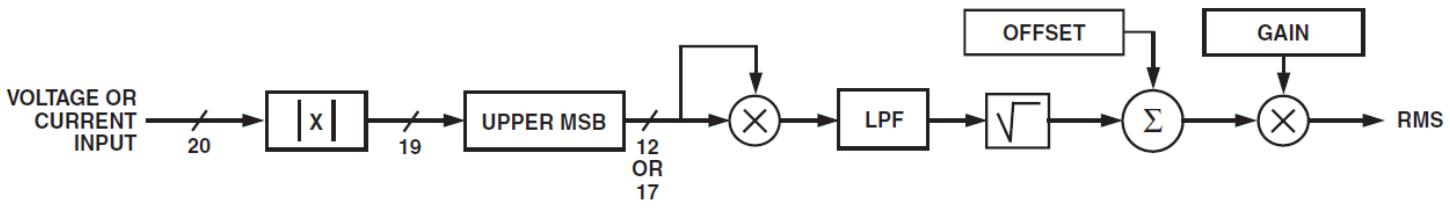
\includegraphics[width=0.75\linewidth]{figs/cislicove_rms.png}
    \caption{Číslicový výpočet RMS.}
    \label{fig:cislicovy-vypocet-rms}
\end{figure}
\end{tcolorbox}

\begin{tcolorbox}[title={\stepcounter{questionnumber}\thequestionnumber. Nakreslete obvod pro změření příkonu žárovky napájené ze zdroje U=10V, svítící žárovka má odpor 10 $\Omega$, způsobí použité reálné přístroje nějakou chybu metody, jak ji případně lze korigovat? (12)}]
\[
I=\frac{U}{R}=\frac{10}{10}=1~\mathrm{A},\qquad P=UI=10~\mathrm{W}
\]
\textbf{Chyba metody vlevo:} ampérmetr měří i proud voltmetrem.
\[
P_Z=U_Z I_A-\frac{U_Z^2}{R_V}
\]
U DMM bývá $R_V$ velký => chyba malá.
\begin{figure}[H]
    \centering
    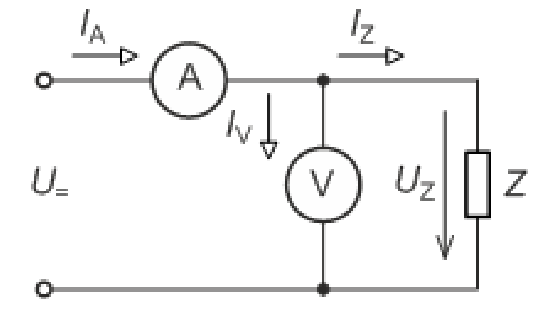
\includegraphics[width=0.4\linewidth]{figs/mereni_vykonu_na_zarovce.png}
    \caption{Měření příkonu žárovky.}
    \label{fig:mereni-prikonu-zarovky}
\end{figure}
\end{tcolorbox}

\begin{tcolorbox}[title={\stepcounter{questionnumber}\thequestionnumber. Nakreslete zapojení pro změření výkonu na žárovce napájené stejnosměrným napětím 10V, vhodné pokud mám k dispozici ideální voltmetr. Jaký bude naměřený výkon, pokud je odpor žárovky při provozu 10 $\Omega$? (12)}]
Ideální voltmetr => $I=U/R=10/10=1~\mathrm{A}$.
\[
P=UI=10\cdot1=10~\mathrm{W}
\]
\begin{figure}[H]
    \centering
    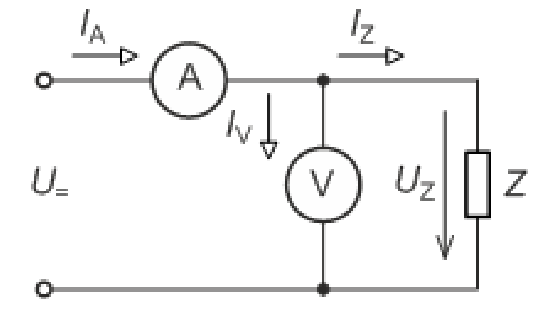
\includegraphics[width=0.4\linewidth]{figs/mereni_vykonu_na_zarovce.png}
    \caption{Měření výkonu žárovky.}
    \label{fig:mereni-vykonu-zarovky}
\end{figure}
\end{tcolorbox}

\begin{tcolorbox}[title={\stepcounter{questionnumber}\thequestionnumber. Jaký vztah platí mezi jalovým, činným a zdánlivým výkonem, jaké jsou jejich jednotky? (16)}]
\[
S=UI~[\mathrm{VA}],\qquad P=UI\cos\varphi~[\mathrm{W}],\qquad Q=UI\sin\varphi~[\mathrm{var}]
\]
\[
S^2=P^2+Q^2
\]
Pro neharmonické průběhy: $S^2=P^2+Q^2+D^2$.
\end{tcolorbox}

\begin{examplebox}[title={Výkon v obvodu se zátěží s fázovým posunem}]
\textbf{Otázka:} Pro $u(t)=\sqrt{2}U\sin(\omega t)$ a $i(t)=\sqrt{2}I\sin(\omega t+\varphi)$ určete $S$, $P$, $Q$ a účiník. Co se mění u neharmonických průběhů?\\
\textbf{Odpověď:}
\[
S=UI,\qquad P=UI\cos\varphi,\qquad Q=UI\sin\varphi,\qquad \lambda=\frac{P}{S}=\cos\varphi
\]
Neharmonický průběh => přibývá deformační výkon $D$:
\[S^2=P^2+Q^2+D^2\]
\end{examplebox}

\begin{tcolorbox}[title={\stepcounter{questionnumber}\thequestionnumber. Pokud vím, že na zátěži je zdánlivý výkon S=100 VA a fázový posun mezi napětím a proudem je cca 85°, bude činný výkon spíše blíže 0 W nebo 100 W (vysvětlete proč). (16)}]
\[
P=S\cos\varphi=100\cos85^\circ\approx8{,}7~\mathrm{W}
\]
=> blíže $0~\mathrm{W}$, protože $\cos85^\circ$ je malý.
\end{tcolorbox}

\begin{tcolorbox}[title={\stepcounter{questionnumber}\thequestionnumber. Jaký je vztah mezi činným a zdánlivým výkonem v obvodech střídavého proudu, jaké mají jednotky, jak se změří? (13-16)}]
\[
P=S\cos\varphi,\qquad S=U_{RMS}I_{RMS}
\]
\textbf{Jednotky:} $P$ [W], $S$ [VA].\\
\textbf{Měření:} $P$ wattmetrem nebo číslicově jako průměr okamžitého výkonu:
\[
P=\overline{p(t)}=\overline{u(t)i(t)}
\]
$S$ z efektivních hodnot napětí a proudu.
\end{tcolorbox}

\begin{tcolorbox}[title={\stepcounter{questionnumber}\thequestionnumber. Jaký naměříme činný výkon na ideálním kondenzátoru C=1 $\mu$F napájeném ze zdroje napětí U=230 VAC? (14, 15, 16)}]
Ideální kondenzátor: proud předbíhá napětí o $90^\circ$.
\[
P=UI\cos90^\circ=0~\mathrm{W}
\]
\end{tcolorbox}

\begin{tcolorbox}[title={\stepcounter{questionnumber}\thequestionnumber. Jaký bude činný výkon na zátěži tvořené kondenzátorem o kapacitě 100 nF, pokud bude připojena na zdroj sinusového napětí o napětí u=100·sin($\omega$t) (V) pro $\omega$ = 100$\pi$ (rad). (14-16)}]
Ideální kondenzátor => $\varphi=90^\circ$.
\[
P=UI\cos90^\circ=0~\mathrm{W}
\]
\end{tcolorbox}

\begin{tcolorbox}[title={\stepcounter{questionnumber}\thequestionnumber. Jak se principiálně měří činný výkon v moderním elektronickém elektroměru? Popište algoritmus pro nesynchronní vzorkování. (19–21)}]
Vzorkuje se $u[n]$ a $i[n]$, vzorky se násobí:
\[
p[n]=u[n]i[n]
\]
Průměr/integrace se nahradí číslicovou dolní propustí:
\[
P\approx\frac{1}{N}\sum_{n=1}^{N}u[n]i[n]
\]
Není nutné znát přesnou síťovou frekvenci; funguje i pro neharmonické periodické průběhy.
\begin{figure}[H]
    \centering
    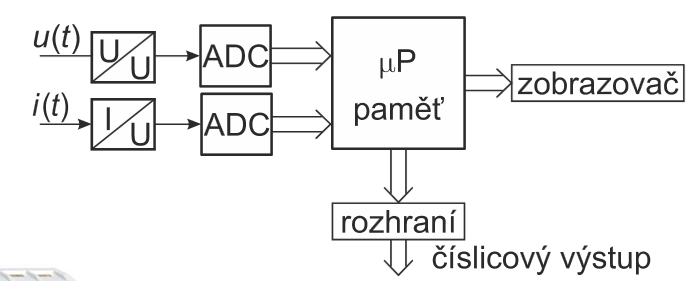
\includegraphics[width=0.5\linewidth]{figs/wattmere_cislicovy.png}
    \caption{Číslicový wattmetr.}
    \label{fig:cislicovy-wattmetr}
\end{figure}
\end{tcolorbox}

% ---------------------------------------------------------
% 4 — Měření odporu a malých napětí – senzory teploty
% ---------------------------------------------------------
\newpage
\section*{4. Měření odporu a malých napětí – senzory teploty}
\setcounter{chapternumber}{4}
\setcounter{questionnumber}{0}
% ---------------------------------------------------------

\begin{tcolorbox}[title={\stepcounter{questionnumber}\thequestionnumber. Co měří a jak funguje senzor PT100, co vyjadřuje jeho jméno “PT100”? Jaký obvod byste použili pro měření s ním? (3, 4, 17)}]
\textbf{PT100:} platinový odporový teploměr, $R_0=100~\Omega$ při $0^\circ\mathrm{C}$.\\
\textbf{Princip:} odpor Pt roste s teplotou:
\[
R=R_0(1+\alpha\vartheta),\qquad \alpha\approx0{,}39\%/K
\]
\textbf{Měření:} zdroj konstantního proudu + voltmetr, ideálně 4vodičově. Typicky PT100 $I<1~\mathrm{mA}$ kvůli samoohřevu.
\end{tcolorbox}

\begin{examplebox}[title={PT100 – lineární aproximace}]
\textbf{Otázka:} Pro PT100 použijte $R=R_0(1+\alpha\vartheta)$, $R_0=100~\Omega$, $\alpha=0{,}39\%/K$. Vypočtěte $R$ při 25, 80 a 100 $^\circ$C a teplotu pro $R=119{,}5~\Omega$.\\
\textbf{Odpověď:}
\[
R_{25}=109{,}75~\Omega,\quad R_{80}=131{,}2~\Omega,\quad R_{100}=139~\Omega
\]
\[
\vartheta=\frac{R/R_0-1}{\alpha}=\frac{119{,}5/100-1}{0{,}0039}=50^\circ\mathrm{C}
\]
\end{examplebox}

\begin{tcolorbox}[title={\stepcounter{questionnumber}\thequestionnumber. Na jakém principu funguje Ohm-metr integrovaný v DMM (např. při měření Rx=100 $\Omega$ a Rx=100 k$\Omega$)? (6)}]
DMM pustí do $R_x$ známý proud a měří úbytek napětí:
\[
R_x=\frac{U}{I_{const}}
\]
Proud se mění podle rozsahu, např. větší proud pro malé odpory, menší proud pro velké odpory.
\end{tcolorbox}

\begin{tcolorbox}[title={\stepcounter{questionnumber}\thequestionnumber. Jak funguje 4-svorková metoda měření odporu - jaké rušivé vlivy se mohou uplatnit? (7)}]
Proud teče proudovými vodiči, napětí se měří samostatnými napěťovými vodiči přímo na $R_x$ => odpory přívodů se neuplatní.\\
\textbf{Termoelektrická napětí:} komutace proudu (měří se v obou polaritách):
\[
U_{mV1}=IR_x+U_{t1}-U_{t2},\qquad U_{mV2}=-IR_x+U_{t1}-U_{t2}
\]
\[
U_x=\frac{U_{mV1}-U_{mV2}}{2}=IR_x
\]
\begin{figure}[H]
    \centering
    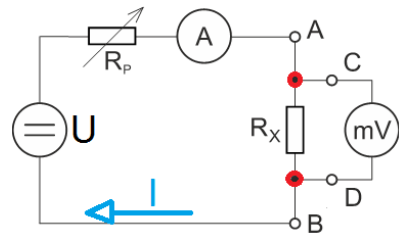
\includegraphics[width=0.4\linewidth]{figs/ctyrsvorka.png}
    \caption{4-svorková metoda.}
    \label{fig:4-svorkova-metoda}
\end{figure}
\end{tcolorbox}

\begin{examplebox}[title={Měření odporu Ohmovou metodou}]
\textbf{Otázka:} Nakreslete zapojení Ohmovy metody pro velmi velké odpory a pro malé/střední odpory. Určete chybu metody.\\
\textbf{Odpověď:}
\begin{figure}[H]
    \centering
    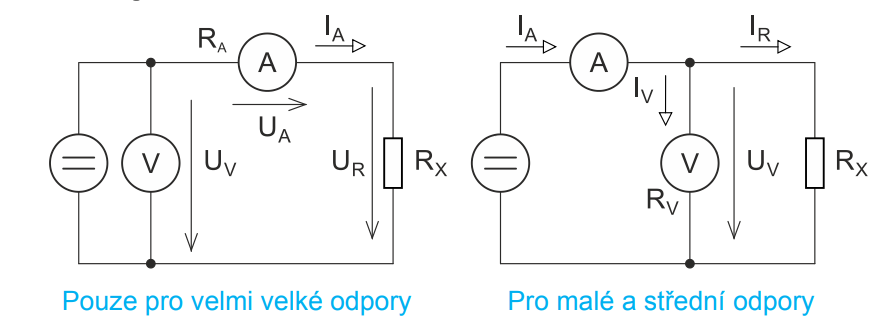
\includegraphics[width=0.5\linewidth]{figs/ohmova_metoda.png}
    \caption{Měření odporu Ohmovou metodou.}
    \label{fig:mereni-odporu-ohmovou-metodou}
\end{figure}
\textbf{Velké odpory:} korigovat odpor ampérmetru:
\[
R_x=\frac{U_V-U_A}{I_A}=\frac{U_V}{I_A}-R_A
\]
\textbf{Malé/střední odpory:} korigovat proud voltmetrem:
\[
R_x=\frac{U_V}{I_A-I_V}=\frac{U_V}{I_A-U_V/R_V}
\]
\end{examplebox}

\begin{tcolorbox}[title={\stepcounter{questionnumber}\thequestionnumber. Nakreslete schéma pro měření malých odporů. Jak se kompenzuje vliv odporu přívodů a termoelektrických napětí? (7)}]
\textbf{Malé odpory:} 4svorková metoda. Odpory přívodů se neuplatní, protože voltmetrem neteče proud.\\
\textbf{Termonapětí:} měření pro $+I$ a $-I$:
viz 4-svorková metoda výše.
\end{tcolorbox}

\begin{tcolorbox}[title={\stepcounter{questionnumber}\thequestionnumber. Na schématu popište metodu měření velmi vysokých odporů s použitím triaxiálního kabelu. Proč takový kabel musíme použít? (9, 10)}]
U velkých odporů jsou proudy pA až fA => vadí svodové proudy izolací.\\
\textbf{Triax:} vnitřní vodič = signál, guard = stejný potenciál jako signál, vnější stínění = zem.\\
Mezi signálem a guardem není napěťový rozdíl => svod neteče do měřicího vstupu.
\begin{figure}[H]
    \centering
    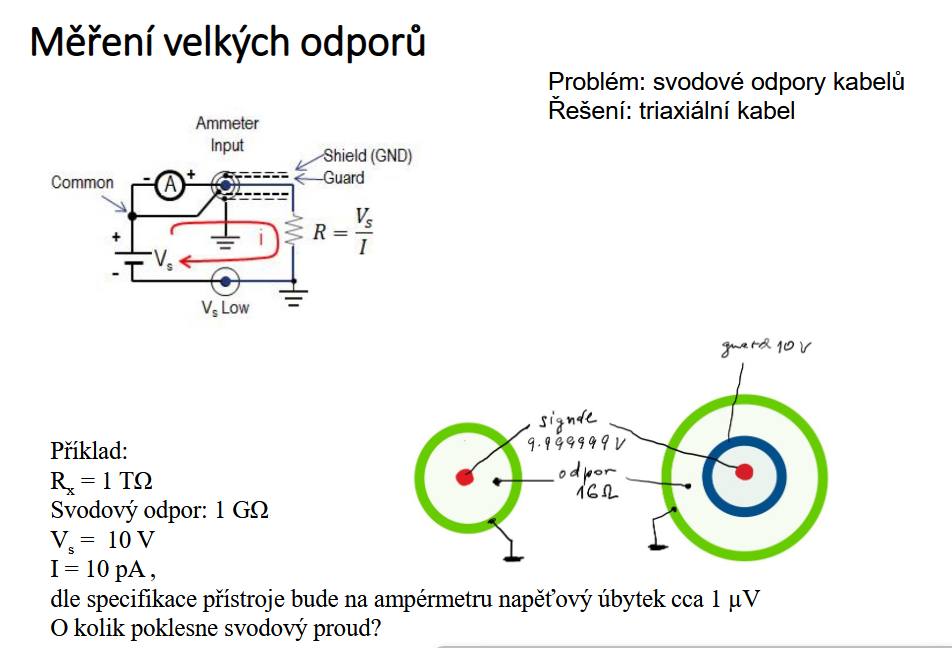
\includegraphics[width=0.5\linewidth]{figs/koax.png}
    \caption{Triaxiální kabel.}
    \label{fig:triaxialni-kabel}
\end{figure}
\end{tcolorbox}

\begin{tcolorbox}[title={\stepcounter{questionnumber}\thequestionnumber. Nakreslete zdroj konstantního proudu, který do zátěže Z (např. senzor PT100) dodá proud 1mA. (12, 17)}]
Invertující zdroj proudu s OZ:
\[
I_Z=-\frac{U_{REF}}{R_{REF}}
\]
Pro $U_{REF}=5~\mathrm{V}$ a $I_Z=1~\mathrm{mA}$:
\[
R_{REF}=\frac{5}{10^{-3}}=5~\mathrm{k\Omega}
\]
\begin{figure}[H]
    \centering
    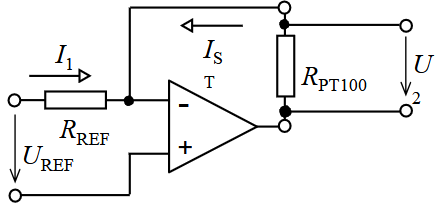
\includegraphics[width=0.5\linewidth]{figs/zdroj_proudu.png}
    \caption{Zdroj proudu.}
    \label{fig:zdroj-proudu}
\end{figure}
\end{tcolorbox}

\begin{examplebox}[title={Zdroj proudu s operačním zesilovačem}]
\textbf{Otázka:} Navrhněte invertující a neinvertující zdroj proudu s OZ. Odvoďte vztahy. Proč je problém plovoucí zátěž?\\
\textbf{Odpověď:}
\[
\text{invertující: } I_2=-\frac{U_1}{R_1},\qquad
\text{neinvertující: } I_2=\frac{U_1}{R_1}
\]
\textbf{Plovoucí zátěž:} napětí na zátěži nelze měřit přímo proti zemi.
\begin{figure}[H]
    \centering
    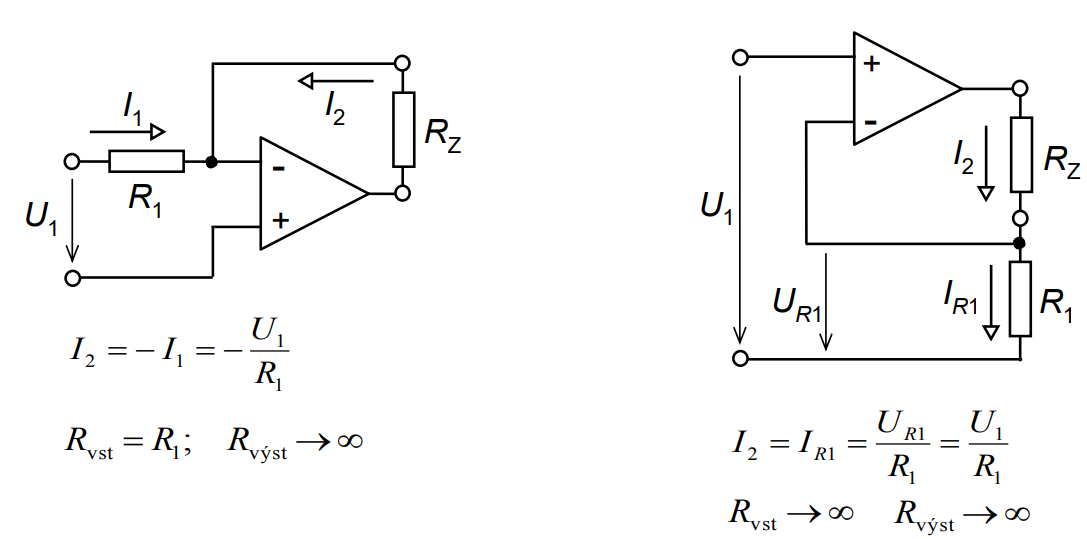
\includegraphics[width=0.5\linewidth]{figs/zdroje_proudu.png}
    \caption{Neinvertující a invertující zdroj proudu.}
    \label{fig:neinvertujici-a-invertujici-zdroj-proudu}
\end{figure}
\end{examplebox}

\begin{examplebox}[title={Integrační zesilovač}]
\textbf{Otázka:} Odvoďte výstup integračního zesilovače s OZ, rezistorem $R$ a kondenzátorem $C$.\\
\textbf{Odpověď:}
\[
u_2(t)=u_2(t_1)-\frac{1}{RC}\int_{t_1}^{t}u_1(\tau)\,d\tau
\]
$u_2(t_1)$ je počáteční napětí na kondenzátoru.
\end{examplebox}

\begin{tcolorbox}[title={\stepcounter{questionnumber}\thequestionnumber. Nakreslete převodník R/U s posunutou nulou a odvoďte jeho výstupní napětí. (14)}]
\[
\frac{U_Z/2}{R_0}=-\frac{U_2-U_Z/2}{R_0+\Delta R}, \qquad
U_2=-U_Z\frac{\Delta R}{2R_0}
\]
\begin{figure}[H]
    \centering
    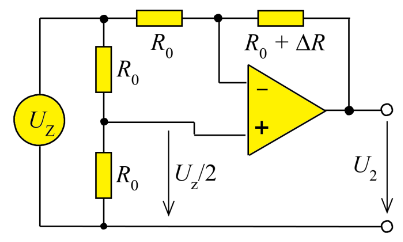
\includegraphics[width=0.5\linewidth]{figs/prevodnik_s_posunutou_nulou.png}
    \caption{Převodník R/U s posunutou nulou.}
    \label{fig:prevodnik-r-u-s-posunutou-nulou}
\end{figure}
\end{tcolorbox}

\begin{examplebox}[title={Převodník R/U s posunutou nulou}]
\textbf{Otázka:} PT100: $R_{0^\circ C}=100~\Omega$, $R_{100^\circ C}=138{,}51~\Omega$. Nastavte $U_Z$ pro $|U_2|=100$ mV při 100 $^\circ$C.\\
\textbf{Odpověď:}
\[
\Delta R=38{,}51~\Omega,\qquad |U_Z|=\frac{2R_0|U_2|}{\Delta R}=\frac{2\cdot100\cdot0{,}1}{38{,}51}=0{,}519~\mathrm{V}
\]
Znaménko $U_2$ závisí na polaritě zapojení.
\end{examplebox}

\begin{tcolorbox}[title={\stepcounter{questionnumber}\thequestionnumber. Nakreslete libovolný obvod, který Vám umožní změřit teplotu laboratorní pícky osazenou senzorem PT100. (17)}]
4vodičově, zdroj konstantního proudu + voltmetr, převodník R/U s posunutou nulou
\end{tcolorbox}

\begin{examplebox}[title={PT100 – návrh čtyřvodičového měřicího obvodu}]
\textbf{Otázka:} $I_{ST}=1$ mA, $U_{REF}=5$ V. Určete $R_{REF}$ a napětí na PT100 při 0 a 100 $^\circ$C.\\
\textbf{Odpověď:}
\[
I_{ST}=-\frac{U_{REF}}{R_{REF}},\qquad R_{REF}=5~\mathrm{k\Omega}
\]
\[
U_{0^\circ C}=1~\mathrm{mA}\cdot100~\Omega=100~\mathrm{mV}
\]
\[
U_{100^\circ C}=1~\mathrm{mA}\cdot138{,}51~\Omega=138{,}51~\mathrm{mV}
\]
\end{examplebox}

\begin{examplebox}[title={PT100 – výpočet teploty a nejistoty}]
\textbf{Otázka:} $U_2=189{,}384$ mV, $I_{ST}=1$ mA, $\alpha=0{,}39\%/K$. Určete $R$, $\vartheta$ a rozšířenou nejistotu odporu.\\
\textbf{Odpověď:}
\[
R_{PT100}=\frac{0{,}189384}{10^{-3}}=189{,}384~\Omega
\]
\[
\vartheta=\frac{189{,}384/100-1}{0{,}0039}=229{,}2^\circ\mathrm{C}
\]
Ze slidů pro dané tolerance:
\[
u_R=0{,}17~\Omega,\qquad U_R=k_ru_R=0{,}34~\Omega
\]
\end{examplebox}

\begin{tcolorbox}[title={\stepcounter{questionnumber}\thequestionnumber. Poměrová metoda měření odporu AD převodníkem – nakreslete a stručně vysvětlete. Jakou má tato metoda výhodu? Odvoďte. (19)}]
ADC má integrovaný \textbf{zdroj proudu} $I_{\mathrm{EXC}}$, který teče sériově
přes referenční rezistor $R_{\mathrm{Ref}}$ a měřený odpor senzoru $R_{\mathrm{RTD}}$.
Měří se dvě napětí:


\[
V_{\mathrm{RTD}} = R_{\mathrm{RTD}} \cdot I_{\mathrm{EXC}}, \qquad
V_{\mathrm{Ref}} = R_{\mathrm{Ref}} \cdot I_{\mathrm{EXC}}.
\]



Z kódu převodníku pak:


\[
R_{\mathrm{RTD}} = \frac{\mathrm{Code}_{\mathrm{RTD}}}{\mathrm{Code}_{\mathrm{ADC\_Fullscale}}}
\cdot R_{\mathrm{Ref}}.
\]



\textbf{Výhoda:}
Nestabilita proudu $I_{\mathrm{EXC}}$ se \emph{zcela vyruší}, protože je v čitateli
i jmenovateli. Zapojení zároveň funguje jako \textbf{4vodičové} měření odporu
s vysokým rozlišením (typicky až $\sim 18$ bitů).
\begin{figure}[H]
    \centering
    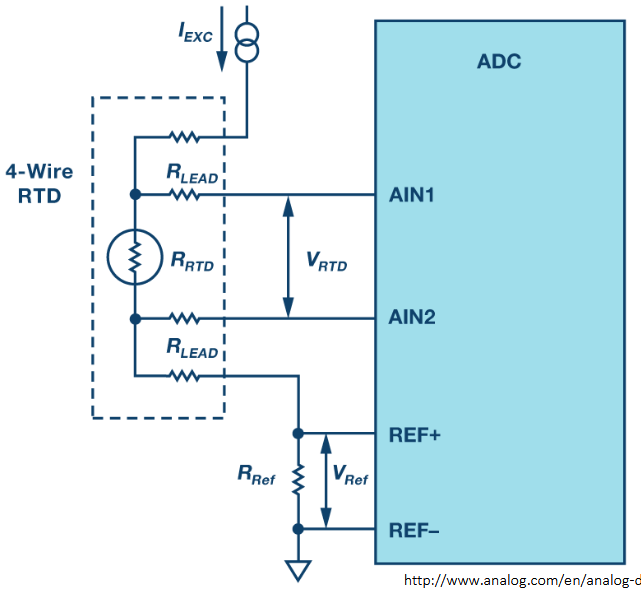
\includegraphics[width=0.5\linewidth]{figs/pomerovametoda.png}
    \caption{Poměrová metoda měření R.}
    \label{fig:pomerova-metoda-mereni-r}
\end{figure}
\end{tcolorbox}

\begin{tcolorbox}[title={\stepcounter{questionnumber}\thequestionnumber. Co je tenzometr, jak se umísťuje, zapojuje, k čemu slouží? (24–31)}]
\textbf{Tenzometr:} odporový senzor deformace. Při deformaci se mění $l$, $S$ a $\rho$:
\[
R=\rho\frac{l}{S}
\]
Lepí se na měřený díl ve směru deformace. Malé změny odporu => Wheatstoneův můstek.\\
\textbf{Použití:} síla, tlak, hmotnost, krouticí moment, zatížení konstrukcí.
\end{tcolorbox}

\begin{examplebox}[title={Tenzometr – deformační citlivost}]
\textbf{Otázka:} Odvoďte vztah pro relativní změnu odporu a definujte $K$.\\
\textbf{Odpověď:}
\[
\frac{\Delta R}{R}=\frac{\Delta l}{l}-\frac{\Delta S}{S}+\frac{\Delta\rho}{\rho}
\]
\[
K=\frac{\Delta R/R}{\Delta l/l}=1+2\mu+\frac{\Delta\rho/\rho}{\Delta l/l},\qquad \varepsilon=\frac{\Delta l}{l}
\]
Pro kovové tenzometry typicky $K\approx2$.
\end{examplebox}

\begin{tcolorbox}[title={\stepcounter{questionnumber}\thequestionnumber. Jaký je princip, jak funguje a co měří tenzometr, jaké provedení je nejběžnější. Zapojení do měřicího obvodu? (24–33)}]
Měří relativní deformaci $\varepsilon$ přes změnu odporu:
\[
\frac{\Delta R}{R}=K\varepsilon
\]
Nejběžnější: lepený fóliový tenzometr. 
\begin{figure}[H]
    \centering
    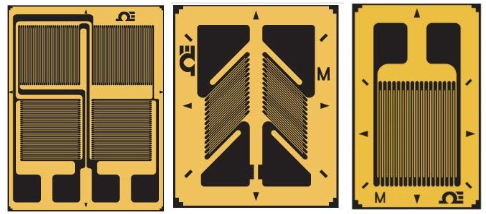
\includegraphics[width=0.25\linewidth]{figs/tenometr.png}
    \caption{Tenzometr.}
    \label{fig:tenzometr}
\end{figure}
\end{tcolorbox}

\begin{examplebox}[title={Tenzometrický snímač – zatížení 1000 kg}]
\textbf{Otázka:} Úplný můstek, $U_Z=5$ V, proud v nezatíženém můstku 10 mA, $U_V=2$ mV, $K=2$, $l=5$ mm.\\
\textbf{Odpověď:}
\[
R=\frac{U_Z}{I}=\frac{5}{0{,}01}=500~\Omega
\]
\[
U_V=U_Z\frac{\Delta R}{R}\Rightarrow \Delta R=\frac{U_V}{U_Z}R=\frac{0{,}002}{5}\cdot500=0{,}2~\Omega
\]
\[
\varepsilon=\frac{\Delta R/R}{K}=\frac{0{,}2/500}{2}=2\cdot10^{-4},\qquad \Delta l=\varepsilon l=1~\mu\mathrm{m}
\]
\end{examplebox}

\begin{tcolorbox}[title={\stepcounter{questionnumber}\thequestionnumber. Jak se odpory na defofrmačním členu (tenzometry) umístí do můstku? (32)}]
Tenzometry s deformací opačného znaménka se zapojí tak, aby se změny v měřicí diagonále sčítaly. Stejné teplotní změny se v můstku kompenzují.
\begin{figure}[H]
\centering
\begin{minipage}{0.45\linewidth}
    \centering
    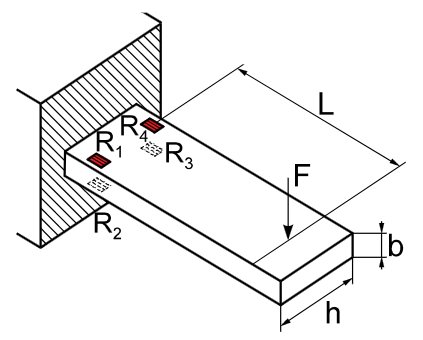
\includegraphics[width=\linewidth]{figs/mustek_tenzometr.png}
\end{minipage}
\hfill
\begin{minipage}{0.45\linewidth}
    \centering
    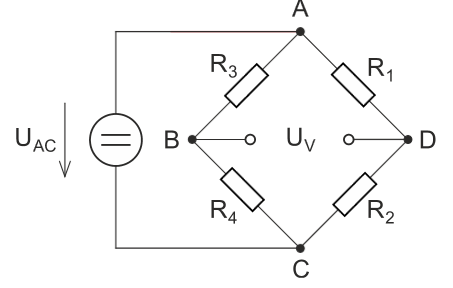
\includegraphics[width=\linewidth]{figs/mustek.png}
\end{minipage}
\end{figure}
\end{tcolorbox}

\begin{tcolorbox}[title={\stepcounter{questionnumber}\thequestionnumber. Nakreslete poloviční Wheatstoneův můstek a odvoďte jeho výstupní napětí pro proudové napájení. (31)}]

\begin{figure}[H]
    \centering
    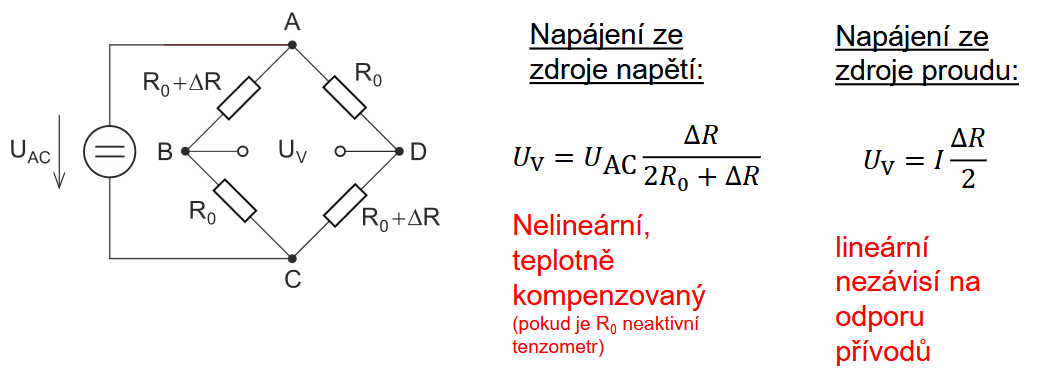
\includegraphics[width=0.8\linewidth]{figs/mustek_pol.png}
    \caption{Poloviční Wheatstoneův můstek.}
    \label{fig:polovicni-wheatstoneuv-mustek}
\end{figure}
\end{tcolorbox}

\begin{tcolorbox}[title={\stepcounter{questionnumber}\thequestionnumber. Nakreslete úplný Wheatstoneův můstek a odvoďte jeho výstupní napětí pro proudové napájení. (31)}]

\begin{figure}[H]
    \centering
    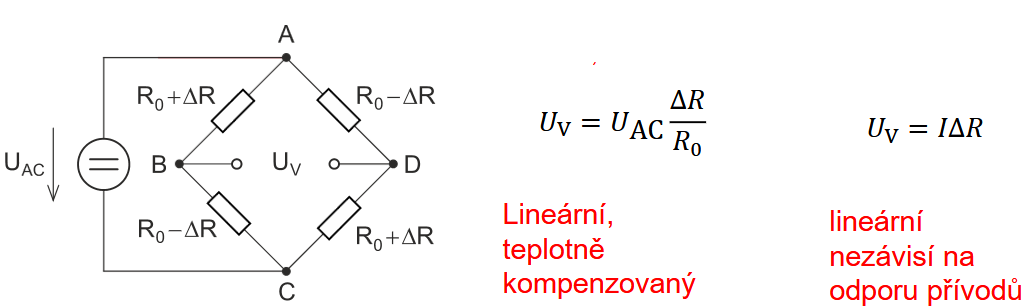
\includegraphics[width=0.8\linewidth]{figs/mustekcely.png}
    \caption{Celý Wheatstoneův můstek.}
    \label{fig:cely-wheatstoneuv-mustek}
\end{figure}
\end{tcolorbox}

\begin{examplebox}[title={Tenzometrický můstek – úplný můstek}]
\textbf{Otázka:} Úplný můstek, $U_Z=1$ V, $R_0=500~\Omega$, $K=2{,}05$, $U_2=200~\mu$V. Určete deformaci.\\
\textbf{Odpověď:}
\[
U_2=U_Z\frac{\Delta R}{R}=U_ZK\frac{\Delta l}{l}
\]
\[
\frac{\Delta l}{l}=\frac{U_2}{U_ZK}=\frac{200\cdot10^{-6}}{1\cdot2{,}05}=97{,}5\cdot10^{-6}
\]
\end{examplebox}

\begin{examplebox}[title={Tenzometrický můstek – nejistota měření}]
\textbf{Otázka:} $A=1000\pm1$, ADC rozsah 5 V, chyba $\pm0{,}025\%$ rozsahu, $K$ tolerance 0,3 \%, $U_Z=1\pm0{,}001$ V.\\
\textbf{Odpověď:} Ze slidů:
\[
u_{U_2}=0{,}73~\mu\mathrm{V},\qquad u_{\Delta l/l}=0{,}4\cdot10^{-6}
\]
Relativně k $97{,}5\cdot10^{-6}$:
\[
\frac{u_{\Delta l/l}}{\Delta l/l}\approx0{,}4\%
\]
\end{examplebox}

\begin{tcolorbox}[title={\stepcounter{questionnumber}\thequestionnumber. V nevyváženém Wheatstoneově můstku je zapojen jeden neznámý odpor Rx a tři známé odpory R. Můstek je napájen ze zdroje napětí U. Jaké bude výstupní napětí můstku? Nakreslete a odvoďte. (31)}]
Pro $R_x=R_0+\Delta R$, ostatní $R_0$:
\[
U_{BD}=U\left(\frac{R_0+\Delta R}{2R_0+\Delta R}-\frac{1}{2}\right)
=U\frac{\Delta R}{4R_0\left(1+\Delta R/(2R_0)\right)}
\]
Pro $\Delta R\ll R_0$:
\[
U_{BD}\approx U\frac{\Delta R}{4R_0}
\]
\begin{figure}[H]
    \centering
    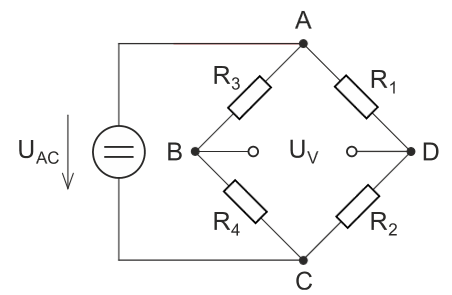
\includegraphics[width=0.4\linewidth]{figs/mustekwh.png}
    \caption{Wheatstoneův můstek.}
    \label{fig:wheatstoneuv-mustek}
\end{figure}
\end{tcolorbox}

\begin{examplebox}[title={Wheatstoneův můstek – převod $\Delta R$ na napětí}]
\textbf{Otázka:} Jeden aktivní odpor $R_1=R_0+\Delta R$, ostatní $R_0$. Odvoďte výstup pro napěťové a proudové napájení.\\
\textbf{Odpověď:}
\[
U_{BD}=U_{AC}\frac{\Delta R}{4R_0\left(1+\Delta R/(2R_0)\right)}
\]
\[
U_{BD}=\frac{I_Z}{4}\frac{\Delta R}{1+\Delta R/(4R_0)}
\]
\end{examplebox}

\begin{examplebox}[title={Diferenční zesilovač pro měření můstku}]
\textbf{Otázka:} Odvoďte výstup pro $R_1=R_2=R_3=R_4$ a podmínku zesílení $k$.\\
\textbf{Odpověď:}
Pro stejné odpory:
\[
U_0=U_2-U_1
\]
Pro zesílení $k$:
\[
\frac{R_2}{R_1}=\frac{R_4}{R_3}=k
\]
Přístrojový zesilovač: vysoký vstupní odpor, vysoké CMRR, nezatěžuje můstek.
\end{examplebox}

\begin{tcolorbox}[title={\stepcounter{questionnumber}\thequestionnumber. Odporový senzor polohy - princip (obrázek), výhody - nevýhody, jak se docílí potlačení změn rezistivity v závislosti na teplotě? (36)}]
Potenciometr = odporový dělič s jezdcem:
\[
U_{out}=U\frac{R_2}{R_1+R_2}
\]
Změna rezistivity se potlačí poměrovým měřením: mění se $R_1$ i $R_2$ stejně.\\
\textbf{Výhody:} jednoduchý, levný, lineární, lze i nelineární průběh.\\
\textbf{Nevýhody:} kontaktní snímač => opotřebení, omezená životnost/rychlost.
\begin{figure}[H]
    \centering
    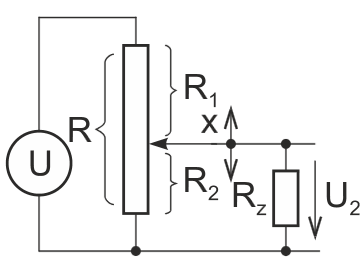
\includegraphics[width=0.25\linewidth]{figs/odposrpolohy.png}
    \caption{Potenciometr.}
    \label{fig:potenciometr}
\end{figure}
\end{tcolorbox}

\begin{examplebox}[title={Potenciometrický snímač polohy – zatížení měřidlem}]
\textbf{Otázka:} $R_P=50$ k$\Omega$, $U=5$ V, jezdec uprostřed, DMM $R_V=10$ M$\Omega$, rozsah 10 V, rozlišení 1 mV, chyba $0{,}05\%$ + 2 digity.\\
\textbf{Odpověď:}
\[
u_B=\frac{0{,}05\%\cdot2{,}5+2\cdot1~\mathrm{mV}}{\sqrt3}=1{,}9~\mathrm{mV}
\]
\[
R_{OUT}=\frac{25\cdot25}{50}~\mathrm{k\Omega}=12{,}5~\mathrm{k\Omega}
\]
\[
\Delta U=-U_1\frac{R_{OUT}}{R_{OUT}+R_V}=-2{,}5\frac{12{,}5k}{12{,}5k+10M}=-3{,}1~\mathrm{mV}
\]
\[
\delta_{MET}=\frac{-3{,}1~\mathrm{mV}}{5~\mathrm{V}}100=-0{,}06\%
\]
\end{examplebox}

\begin{examplebox}[title={Potenciometrický snímač – závislost chyby na poloze}]
\textbf{Otázka:} Odvoďte $R_{OUT}$ pro polohu $x\in\langle0;1\rangle$ a navrhněte oddělení.\\
\textbf{Odpověď:}
\[
R_1=(1-x)R_P,\qquad R_2=xR_P
\]
\[
R_{OUT}=\frac{R_1R_2}{R_1+R_2}=R_Px(1-x)
\]
Chyba zatížením je nulová pro $x=0,1$, maximální pro $x=0{,}5$. Oddělení: napěťový sledovač s OZ ($A=1$, vysoký $R_{in}$).
\end{examplebox}

\begin{tcolorbox}[title={\stepcounter{questionnumber}\thequestionnumber. Co měří a jak funguje termočlánek, pro jaké aplikace se typicky používá? (40, 41)}]
Termočlánek měří rozdíl teplot měřicího a srovnávacího spoje. Teplotní gradient ve dvou různých materiálech => termoelektrické napětí:
\[
U=\int_{T_S}^{T_M}\sigma_{12}(T)\,dT\approx\alpha_{12}(\vartheta_M-\vartheta_S)
\]
\textbf{Použití:} velmi nízké/vysoké teploty, pece, spalování, turbíny, robustní průmyslové měření.
\begin{figure}[H]
    \centering
    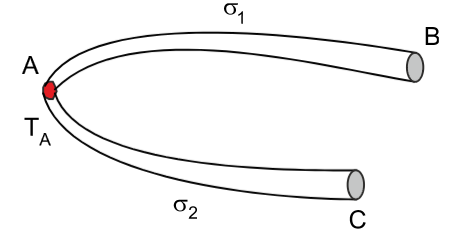
\includegraphics[width=0.5\linewidth]{figs/termoclanek.png}
    \caption{Termočlánek.}
    \label{fig:termoclanek}
\end{figure}
\end{tcolorbox}

\begin{examplebox}[title={Termočlánek – návrh teploměru}]
\textbf{Otázka:} Termočlánek $53~\mu$V/K, výstup 0 V při 0 $^\circ$C a 1 V při 100 $^\circ$C, 16bit ADC 5 V.\\
\textbf{Odpověď:}
\[
U_1(100^\circ C)=100\cdot53~\mu\mathrm{V}=5{,}3~\mathrm{mV}
\]
\[
A=\frac{U_2}{U_1}=\frac{1}{5{,}3\cdot10^{-3}}=188{,}7
\]
Neinvertující zesilovač:
\[
A=1+\frac{R_2}{R_1}\Rightarrow R_1=100~\Omega,\quad R_2\approx18{,}77~\mathrm{k\Omega}
\]
Použít kompenzaci srovnávacího spoje.
\end{examplebox}

\begin{examplebox}[title={Termočlánek – nejistota měření}]
\textbf{Otázka:} Určete rozšířenou nejistotu vstupního napětí pro $U_2=3$ V, tolerance rezistorů 0,1 \%, ADC chyba 4 LSB; potom s offsetem OZ $\pm20~\mu$V.\\
\textbf{Odpověď:}
\[
\Delta U_{ADC}=\frac{5}{2^{16}}\cdot4=305~\mu\mathrm{V},\qquad u_{U2}=176~\mu\mathrm{V}
\]
Ze slidů pro ideální OZ:
\[
u_{U1}=13~\mu\mathrm{V},\qquad U_{U1}=2u_{U1}=26~\mu\mathrm{V}
\]
S offsetem $\pm20~\mu$V:
\[
U_{U1}=2\sqrt{(13~\mu\mathrm{V})^2+\left(\frac{20~\mu\mathrm{V}}{\sqrt3}\right)^2}=35~\mu\mathrm{V}
\]
\end{examplebox}

% ---------------------------------------------------------
% 5 — Magnetické senzory, magnetická měření, transformátory
% ---------------------------------------------------------

\newpage
\section*{5. Magnetické senzory, magnetická měření. Transformátor napěťový a proudový. Bezkontaktní senzory el. proudu.}
\setcounter{chapternumber}{5}
\setcounter{questionnumber}{0}
% ---------------------------------------------------------

\begin{tcolorbox}[title={\stepcounter{questionnumber}\thequestionnumber. Jaké znáte senzory magnetického pole? (heslovitě princip funkce u každého případně jednoduchý obrázek nebo rovnice) – uveďte alespoň tři (4–18)}]
\textbf{Hallova sonda:} Lorentzova síla vychýlí nosiče => $U_H=R_H I B/t$, DC i AC, $\mu$T až T.\\
\textbf{Magnetorezistory AMR/GMR/TMR:} odpor závisí na magnetizaci, DC i AC, typicky $1~\mu$T až $10$ mT.\\
\textbf{Indukční cívka:} $u_i=-N\,d\Phi/dt$ => jen AC pole, pT až T.\\
\textbf{Fluxgate:} modulace permeability jádra, výstup na $2f_{exc}$, DC i AC, pT až mT.\\
\textbf{Další:} magnetooptické senzory, SQUID, NMR.
\end{tcolorbox}

\begin{tcolorbox}[title={\stepcounter{questionnumber}\thequestionnumber. Hallova sonda - princip (heslovitě + obrázek + rovnice) (5)}]
Proud $I$ teče polovodičem v magnetickém poli $B$ => \text{Lorentzova síla} vychýlí nosiče => vznikne \textbf{Hallovo napětí}.
\[
U_H=R_H\frac{IB}{t}
\]
$R_H$ Hallova konstanta, $t$ tloušťka destičky.
\begin{figure}[H]
    \centering
    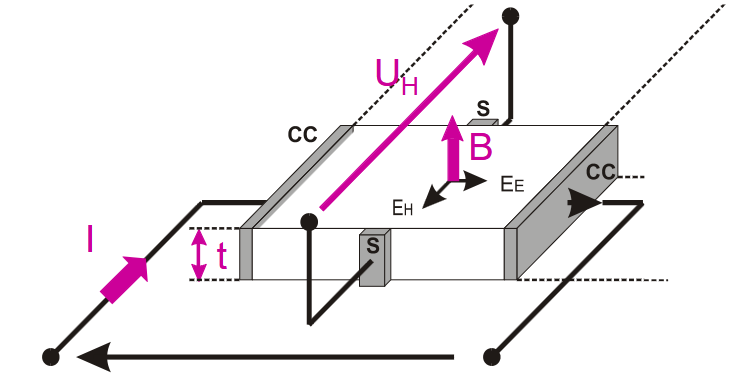
\includegraphics[width=0.5\linewidth]{figs/hall_sonda.png}
    \caption{Hallova sonda.}
    \label{fig:hallova-sonda}
\end{figure}
\end{tcolorbox}

\begin{tcolorbox}[title={\stepcounter{questionnumber}\thequestionnumber. Na jednoduchém obrázku vysvětlete princip Hallova senzoru a napište rovnici pro výstupní napětí. Jaký rozsah magnetických polí může měřit? Uveďte nějakou důležitou aplikaci tohoto senzoru. (5–7)}]
\textbf{Rozsah:} typicky $\mu$T až jednotky T.\\
\textbf{Aplikace:} kompas, bezkontaktní měření proudu, Hallův spínač polohy s permanentním magnetem.
\end{tcolorbox}

\begin{tcolorbox}[title={\stepcounter{questionnumber}\thequestionnumber. Aplikace Hallovy sondy (heslovitě + obrázek) (6–7)}]
...
\end{tcolorbox}

\begin{tcolorbox}[title={\stepcounter{questionnumber}\thequestionnumber. Na jednoduchém obrázku vysvětlete princip AMR magnetorezistoru. Jaký rozsah magnetických polí může měřit? Uveďte nějakou důležitou aplikaci tohoto senzoru. (9–13)}]
\textbf{AMR:} odpor závisí na úhlu mezi proudem a magnetizací $M$. Ve směru $M$ je odpor vyšší, kolmo nižší.\\
\textbf{Změna odporu:} cca 2--3 \%.\\
\textbf{Rozsah:} asi $1$ nT až $10$ mT.\\
\textbf{Aplikace:} elektronický kompas, senzor polohy, proudový senzor.
\begin{figure}[H]
    \centering
    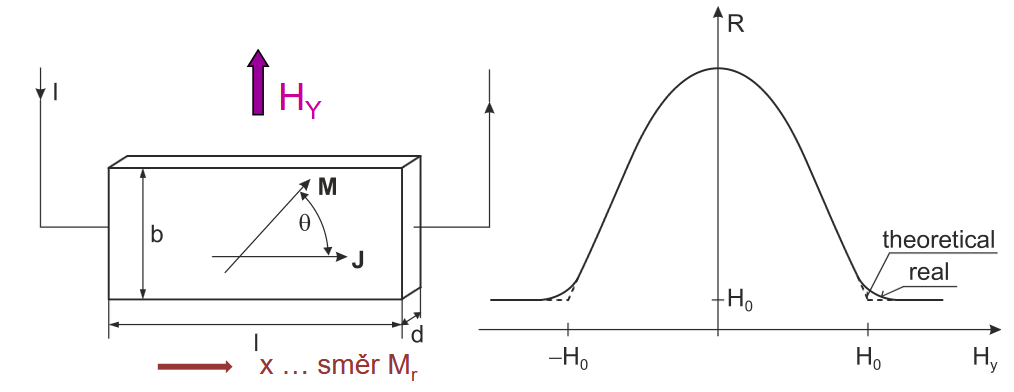
\includegraphics[width=0.75\linewidth]{figs/amr.png}
    \caption{AMR magnetorezistor.}
    \label{fig:amr-magnetorezistor}
\end{figure}
\end{tcolorbox}

\begin{tcolorbox}[title={\stepcounter{questionnumber}\thequestionnumber. AMR senzor – princip, výhody proti Hallově sondě (9–12)}]
\textbf{Proti Hallově sondě:} vyšší citlivost, vhodné pro menší pole, citlivost v rovině čipu.\\
\textbf{Linearizace:} barber-pole struktura nebo posun pracovního bodu; pro offset/drift se používá flipování magnetizace.
\end{tcolorbox}

\begin{tcolorbox}[title={\stepcounter{questionnumber}\thequestionnumber. Jaká je základní rovnice pro indukované napětí u indukčních senzorů a které veličiny lze měnit, aby se dosáhlo požadovaného efektu? Uveďte alespoň tři různé typy senzorů, jejichž funkce je založena na tomto zákoně (2, 15–16)}]
\[
u_i=-\frac{d\Phi}{dt}=-\frac{d}{dt}\left(NS\mu_0\mu_rH\right)
\]
Měnit lze $H(t)$, $S(t)$ nebo $\mu_r(t)$:
\[
u_i\sim NS\mu_0\mu_r\frac{dH}{dt}+N\mu_0\mu_rH\frac{dS}{dt}+NS\mu_0H\frac{d\mu_r}{dt}
\]
\textbf{Příklady:} \textbf{indukční cívka} ($dH/dt$), \textbf{tachodynamo / rotující cívka} ($dS/dt$), \textbf{fluxgate} ($d\mu_r/dt$).
\end{tcolorbox}

\begin{tcolorbox}[title={\stepcounter{questionnumber}\thequestionnumber. Na jednoduchém obrázku vysvětlete princip fluxgate senzoru. Jaký rozsah magnetických polí může měřit? Uveďte nějakou důležitou aplikaci tohoto senzoru. (17–20)}]
Budicí proud periodicky sytí magnetické jádro => mění se $\mu_r(t)$. Měřené DC pole poruší symetrii => ve snímací cívce vznikne složka na $2f_{exc}$.
\[
u_i\sim NS\mu_0H\frac{d\mu_r}{dt}
\]
\textbf{Rozlišení/rozsah:} rozlišení cca $10$ pT, rozsah cca do $2$ mT.\\
\textbf{Aplikace:} přesné magnetometry, družice, geofyzika, fluxgate proudové senzory.
\begin{figure}[H]
    \centering
    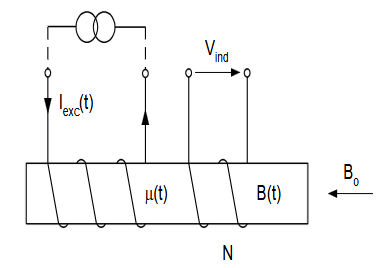
\includegraphics[width=0.5\linewidth]{figs/fluxgate.png}
    \caption{Fluxgate senzor.}
    \label{fig:fluxgate-senzor}
\end{figure}
\end{tcolorbox}

\begin{tcolorbox}[title={\stepcounter{questionnumber}\thequestionnumber. Na jednoduchém obrázku vysvětlete princip ideálního měřicího transformátoru proudu a napište jeho základní rovnici. Jaká je správná zátěž? (24–25)}]

\textbf{Správná zátěž:} malá impedance / téměř zkrat. Sekundár se za provozu nesmí rozpojit.
\begin{figure}[H]
    \centering
    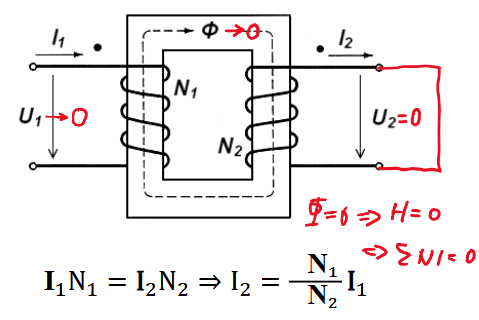
\includegraphics[width=0.5\linewidth]{figs/proudovy_transformator.png}
    \caption{Proudový transformátor.}
    \label{fig:proudovy-transformator}
\end{figure}
\end{tcolorbox}

\begin{tcolorbox}[title={\stepcounter{questionnumber}\thequestionnumber. Na jednoduchém obrázku vysvětlete princip ideálního měřicího transformátoru napětí a napište jeho základní rovnici. Jaká je správná zátěž? (24–25)}]
\textbf{Správná zátěž:} velká impedance / téměř naprázdno.
\begin{figure}[H]
    \centering
    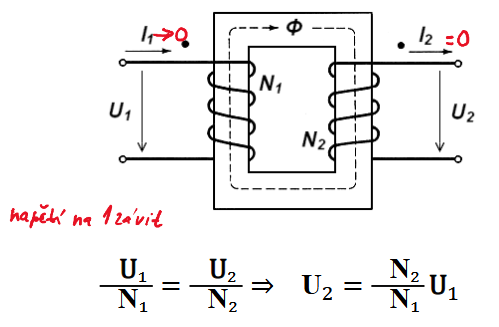
\includegraphics[width=0.5\linewidth]{figs/napetovy_transformator.png}
    \caption{Napěťový transformátor.}
    \label{fig:napetovy-transformator}
\end{figure}
\end{tcolorbox}

\begin{tcolorbox}[title={\stepcounter{questionnumber}\thequestionnumber. Nakreslete zjednodušené náhradní schéma měřicího transformátoru proudu a vysvětlete význam jednotlivých prvků. Označte ty prvky, které jsou pro ideální transformátor proudu nulové a které jsou nekonečně velké. (26)}]
\textbf{NULOVÉ (→ 0):} $R_1$, $R_2'$, $L_{r1}$, $L_{r2}'$, $u_2'$
\textbf{NEKONEČNÉ (→ $\infty$):} $R_{Fe}$, $L_h$ 
\begin{figure}[H]
    \centering
    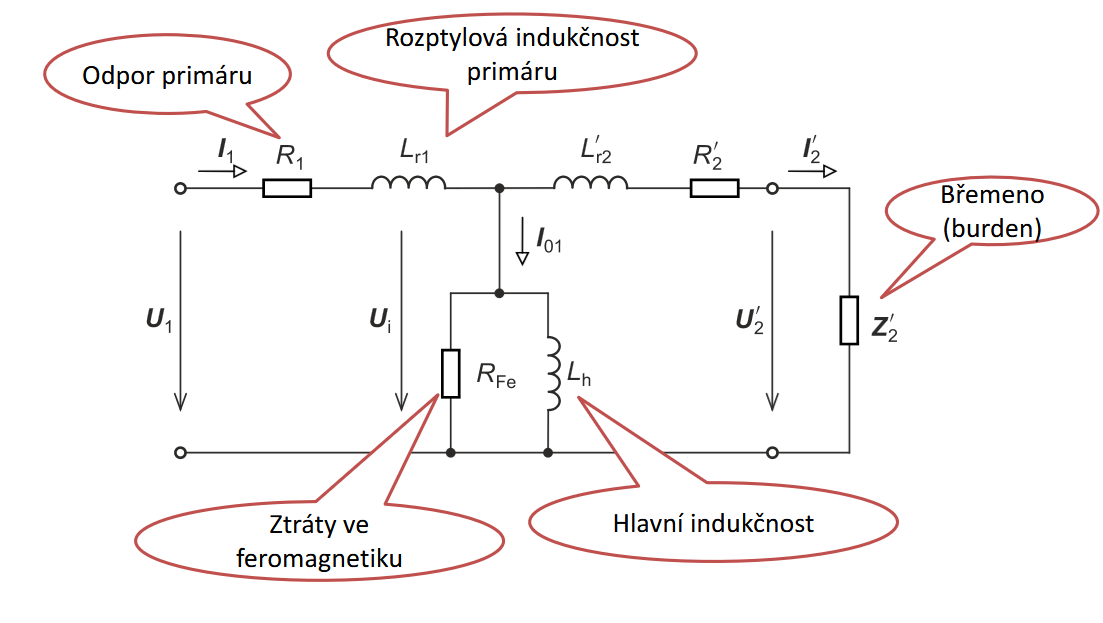
\includegraphics[width=0.75\linewidth]{figs/nahradni_schema.png}
    \caption{Náhradní schéma transformátoru.}
    \label{fig:nahradni-schema-transformatoru}
\end{figure}
\end{tcolorbox}

\begin{tcolorbox}[title={\stepcounter{questionnumber}\thequestionnumber. Popište stručně konstrukci a princip funkce transformátoru napětí, na co se používá? (obrázek, vztah mezi vstupními a výstupními veličinami). Jaké jsou podmínky jeho správné funkce? Co musí být splněno pro nízkou chybu? (27)}]
Dvě vinutí na společném feromagnetickém jádře:
\[
\frac{U_2}{U_1}=\frac{N_2}{N_1}
\]
\textbf{Použití:} měření vysokých napětí, galvanické oddělení.\\
\textbf{Nízká chyba:} velké břemeno $Z_2$ => malý sekundární proud; malé úbytky na odporech a rozptylových indukčnostech; velké $L_h$, velké $R_{Fe}$.
\begin{figure}[H]
    \centering
    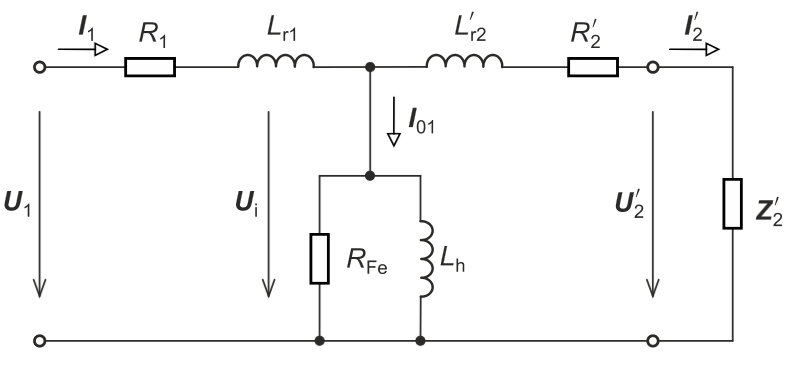
\includegraphics[width=0.75\linewidth]{figs/napetitnf.png}
    \caption{Měřicí transformátor napětí.}
    \label{fig:merici-transformator-napeti}
\end{figure}

\end{tcolorbox}

\begin{tcolorbox}[title={\stepcounter{questionnumber}\thequestionnumber. Popište stručně konstrukci a princip funkce transformátoru proudu, na co se používá? (obrázek, vztah mezi vstupními a výstupními veličinami) Jaké jsou podmínky jeho správné funkce? Co musí být splněno pro nízkou chybu? (28–29)}]
\[
I_1N_1=I_2N_2,\qquad I_2=\frac{N_1}{N_2}I_1
\]
\textbf{Použití:} měření velkých AC proudů, galvanické oddělení, ochrany, elektroměry.\\
\textbf{Nízká chyba:} malé břemeno $Z_2$, velké $L_h$, malé odpory a rozptylové indukčnosti, malé ztráty v jádře.\\
\textbf{Důležité:} sekundár se nesmí rozpojit => vysoké napěťové špičky.
\begin{figure}[H]
    \centering
    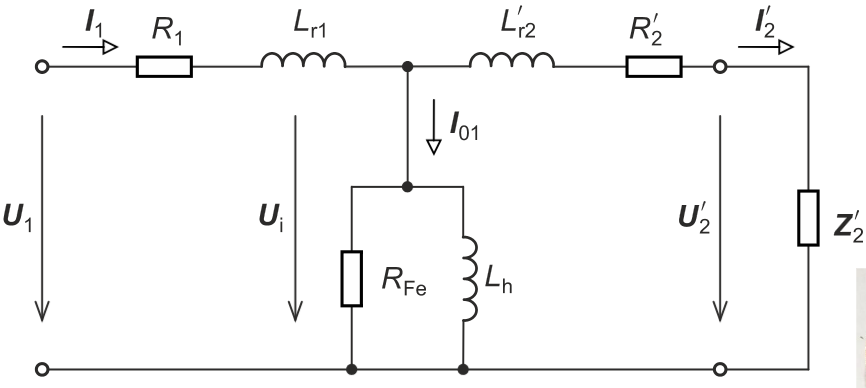
\includegraphics[width=0.75\linewidth]{figs/proudtnf.png}
    \caption{Měřicí transformátor proudu.}
    \label{fig:merici-transformator-proudu}
\end{figure}
\end{tcolorbox}

\begin{tcolorbox}[title={\stepcounter{questionnumber}\thequestionnumber. Jaké znáte senzory elektrického proudu? Uveďte u každého, zda měří ACI, DCI, a je galvanicky oddělen (co to znamená, že senzor je galvanicky oddělen?). (30–39)}]
Galvanické oddělení = mezi měřeným obvodem a výstupem není vodivé spojení.
\begin{center}
\begin{tabular}{|l|c|c|c|}
\hline
\textbf{Senzor} & \textbf{AC} & \textbf{DC} & \textbf{Odděl.} \\
\hline
Bočník & ano & ano & ne \\
Proudový transformátor & ano & ne & ano \\
Převodník I/U & ano & ano & ne \\
Hallův proudový senzor & ano & ano & ano \\
AMR proudový senzor & ano & ano & ano \\
Fluxgate proudový senzor & ano & ano & ano \\
Magnetooptický senzor & ano & ano & ano \\
Rogowského cívka & ano/pulzy & ne & ano \\
\hline
\end{tabular}
\end{center}
\end{tcolorbox}

\begin{tcolorbox}[title={\stepcounter{questionnumber}\thequestionnumber. Jak se měří stejnosměrný elektrický proud bezkontaktně? Uveďte princip a příklady senzorů, které umožňují měřit DC proud. (30–39)}]
DC proud vytvoří statické magnetické pole:
\[
H=\frac{I}{2\pi r}
\]
Bezkontaktně ho měří \textbf{Hall}, \textbf{AMR}, \textbf{fluxgate} nebo \textbf{magnetooptický} senzor.\\
\textbf{Kompenzovaný senzor se jhem:}
\[
n_1I_1=n_2I_2,\qquad I_1=\frac{n_2}{n_1}\frac{U_2}{R_2}
\]
\begin{figure}[H]
    \centering
    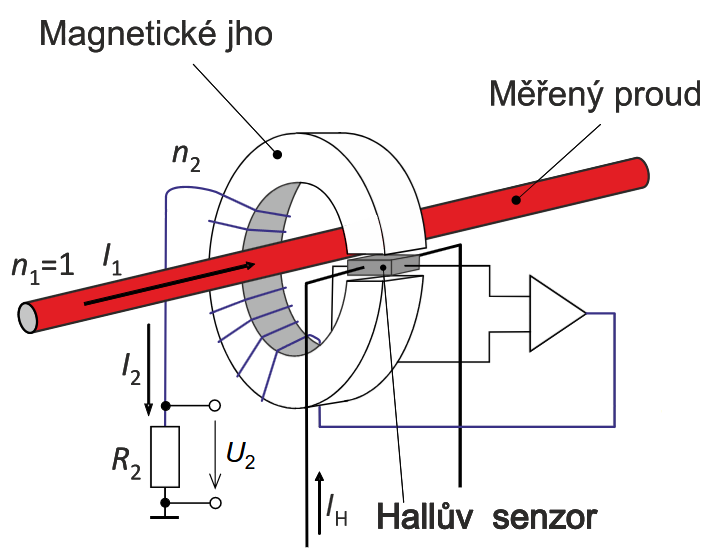
\includegraphics[width=0.5\linewidth]{figs/jho.png}
    \caption{Stacionární proudový senzor se jhem.}
    \label{fig:stacionarni-proudovy-senzor-se-jhem}
\end{figure}
(Místo Hall senzoru může být AMR nebo Fluxgate)

\end{tcolorbox}

\begin{examplebox}[title={Kompenzovaný senzor proudu se jhem}]
\textbf{Otázka:} Odvoďte vztah mezi $I_1$, $I_2$, $n_1$, $n_2$ a výstupním napětím na měřicím rezistoru.\\
\textbf{Odpověď:}
Kompenzační proud ruší tok v jádře:
\[
n_1I_1=n_2I_2
\]
Na měřicím rezistoru:
\[
U_2=R_2I_2
\]
\[
I_1=\frac{n_2}{n_1}I_2=\frac{n_2}{n_1}\frac{U_2}{R_2}
\]
Pro jeden primární průvlek $n_1=1$:
\[
I_1=n_2\frac{U_2}{R_2}
\]
\end{examplebox}

% ---------------------------------------------------------% 6
% ---------------------------------------------------------

\newpage

% ---------------------------------------------------------
% 6 — Měření impedancí, kapacitní a indukčnostní senzory
% ---------------------------------------------------------

\newpage
\section*{6. Měření impedancí, kapacitní a indukčnostní sensory}
\setcounter{chapternumber}{6}
\setcounter{questionnumber}{0}
% ---------------------------------------------------------

\begin{tcolorbox}[title={\stepcounter{questionnumber}\thequestionnumber. Nakreslete jednoduchý převodník Z/U pro měření parametrů sériového náhradního zapojení cívky. Jakým obvodem či přístrojem je třeba měřit jeho výstup? (4–5)}]
Měří se \textbf{reálná i imaginární složka} výstupu => \textbf{synchronní detektor / vektorvoltmetr}.
\begin{figure}[H]
    \centering
    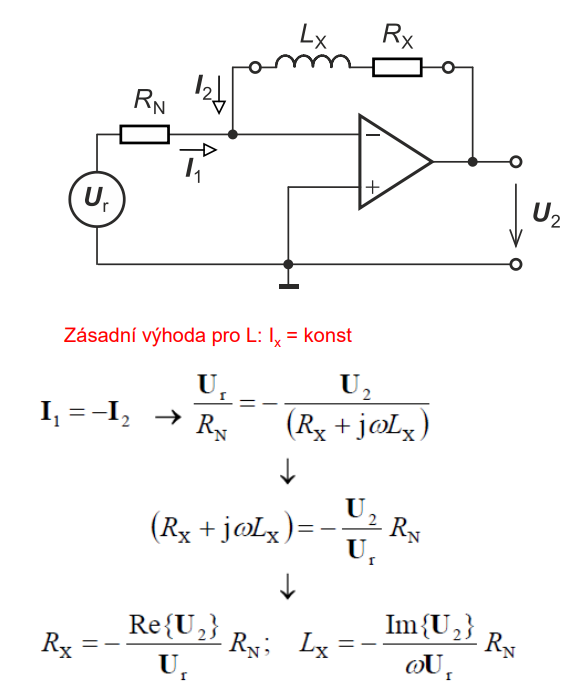
\includegraphics[width=0.5\linewidth]{figs/prevodnik_zu_civka.png}
    \caption{Převodník Z/U pro měření parametrů cívky.}
    \label{fig:prevodnik-z-u-pro-mereni-parametru-civky}
\end{figure}
\end{tcolorbox}

\begin{examplebox}[title={Převodník Z/U}]
\textbf{Otázka:} Navrhněte princip převodníku impedance na napětí. Jak zajistit, aby napětí na referenčním rezistoru bylo reálné?\\
\textbf{Odpověď:}
\[
U_2=-\frac{U_R}{R}Z_x \Rightarrow Z_x=-R\frac{U_2}{U_R}
\]
$U_R$ je na \textbf{čistém referenčním rezistoru} a bere se jako \textbf{fázová reference} pro synchronní detektor. Pak lze z $U_2$ určit \textbf{Re} a \textbf{Im} část $Z_x$.
\end{examplebox}

\begin{tcolorbox}[title={\stepcounter{questionnumber}\thequestionnumber. Nakreslete schéma převodníku indukčnost/napětí pro induktor s nezanedbatelným sériovým odporem Rx. Co musí být použito, abychom změřili Lx i Rx? Odvoďte vztah pro Rx. (4–5)}]
viz. předchozí
\end{tcolorbox}

\begin{tcolorbox}[title={\stepcounter{questionnumber}\thequestionnumber. Nakreslete schéma převodníku kapacita/napětí pro kondenzátor s kapacitou Cx a nezanedbatelným svodem Gx. Co musí být použito, abychom změřili Cx i Gx? Odvoďte vztah pro Gx. (4–5)}]
Měří se \textbf{reálná i imaginární složka} výstupu => \textbf{synchronní detektor / vektorvoltmetr}.
\begin{figure}[H]
    \centering
    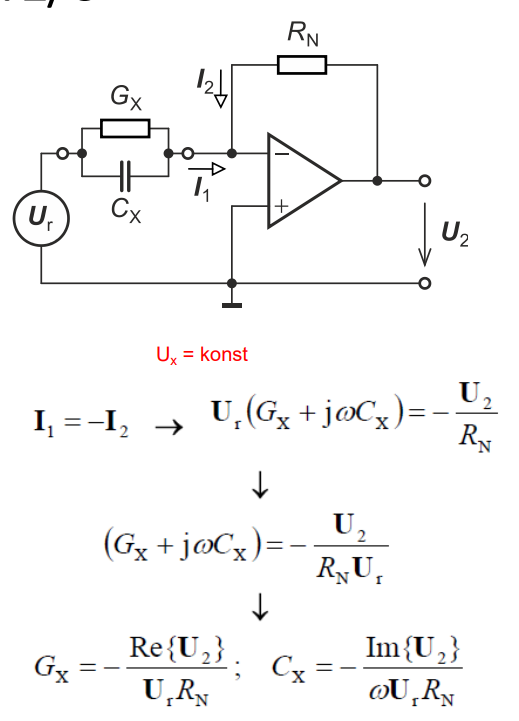
\includegraphics[width=0.5\linewidth]{figs/prevodnik_zu_kondenzator.png}
    \caption{Převodník Z/U pro měření parametrů kondenzátoru.}
    \label{fig:prevodnik-z-u-pro-mereni-parametru-kondenzatoru}
\end{figure}
\end{tcolorbox}

\begin{tcolorbox}[title={\stepcounter{questionnumber}\thequestionnumber. Popište princip funkce kapacitních senzorů (obrázek, rovnice pro C), aplikace? (9–14)}]
\textbf{Princip:} mění se kapacita elektrod:
\[
C=\varepsilon_0\varepsilon_r\frac{S}{d}
\]
Měřená veličina může měnit \textbf{mezeru $d$}, \textbf{plochu překryvu $S$} nebo \textbf{permitivitu $\varepsilon_r$}.\\
\textbf{Aplikace:} poloha/posuv, tlak v MEMS, dotykové ovládání, hladina, bezkontaktní snímání.
\begin{figure}[H]
    \centering
    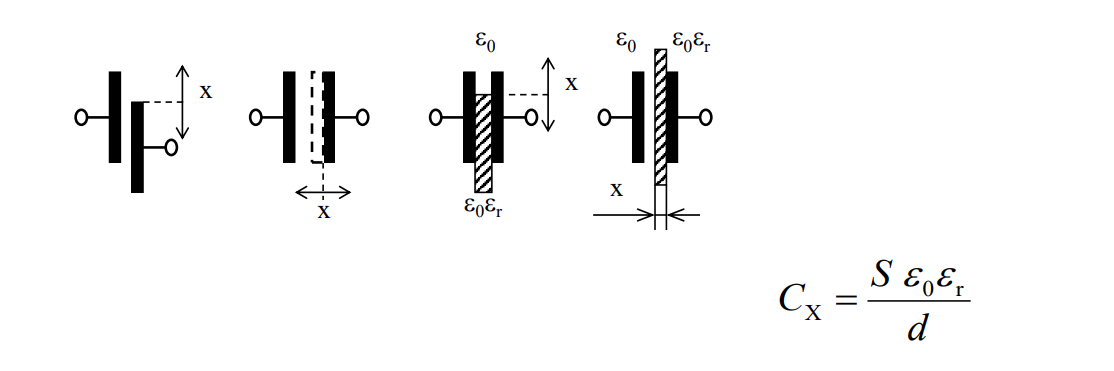
\includegraphics[width=0.5\linewidth]{figs/kapacitni_senzor_polohy.png}
    \caption{Kapacitní senzor polohy.}
    \label{fig:kapacitni-senzor-polohy}
\end{figure}
\end{tcolorbox}

\begin{tcolorbox}[title={\stepcounter{questionnumber}\thequestionnumber. Nakreslete schéma diferenčního kapacitního senzoru s proměnným překryvem elektrod a napište vztah pro obě kapacity C1 a C2. Pomocí diferenční poměrové metody potlačíme teplotní závislosti a výsledná závislost je lineární. Odvoďte. (12)}]
\begin{figure}[H]
    \centering
    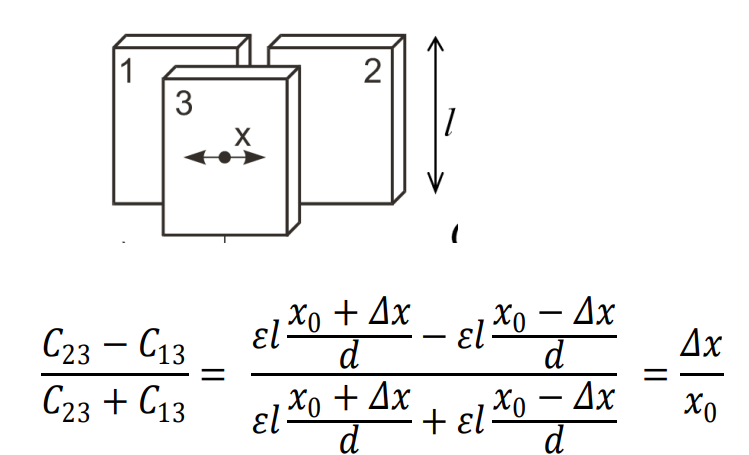
\includegraphics[width=0.5\linewidth]{figs/kapsenzor.png}
    \caption{Kapacitní senzor s proměnnou plochou překrytí.}
    \label{fig:kapacitni-senzor-s-promennou-plochou-prekryti}
\end{figure}
\end{tcolorbox}

\begin{tcolorbox}[title={\stepcounter{questionnumber}\thequestionnumber. Nakreslete schéma diferenčního kapacitního senzoru s proměnnou mezerou a napište vztah pro obě kapacity C1 a C2. Pomocí diferenční poměrové metody potlačíme teplotní závislosti a výsledná závislost je lineární. Odvoďte. (10–11)}]

\begin{figure}[H]
\centering
\begin{minipage}{0.7\linewidth}
    \[
C_1 - C_2
= \varepsilon S \left( \frac{1}{d_0 - \Delta d} - \frac{1}{d_0 + \Delta d} \right)
= \varepsilon S \frac{2\Delta d}{(d_0 - \Delta d)(d_0 + \Delta d)}
\]

\[
C_1 + C_2
= \varepsilon S \left( \frac{1}{d_0 - \Delta d} + \frac{1}{d_0 + \Delta d} \right)
= \varepsilon S \frac{2d_0}{(d_0 - \Delta d)(d_0 + \Delta d)}
\]

\textbf{Diferenční poměrová metoda (linearizace):}

\[
\frac{C_1 - C_2}{C_1 + C_2} = \frac{\Delta d}{d_0}
\]
\end{minipage}
\hfill
\begin{minipage}{0.2\linewidth}
    \centering
    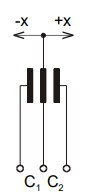
\includegraphics[width=0.6\linewidth]{figs/diferencni_kapacitni_senzor.png}
    \caption{Diferenční kapacitní senzor s proměnnou mezerou.}
    \label{fig:diferencni-kapacitni-senzor-s-promennou-mezerou}
\end{minipage}
\end{figure}
\end{tcolorbox}

\begin{examplebox}[title={Diferenční kapacitní senzor – poměrová metoda}]
\textbf{Otázka:} Pro kapacity $C_1$ a $C_2$ odvoďte výstup poměrového vyhodnocení. Proč metoda potlačuje nelinearitu a teplotu?\\
\textbf{Odpověď:}
\[
U_{out}\sim\frac{C_1-C_2}{C_1+C_2}
\]
Pro proměnnou mezeru:
\[
U_{out}\sim\frac{\Delta d}{d_0}
\]
Pro proměnný překryv:
\[
U_{out}\sim\frac{\Delta x}{x_0}
\]
Společné násobky kapacit ($\varepsilon$, plocha, teplotní změny) jsou v čitateli i jmenovateli => \textbf{vykrátí se}.
\end{examplebox}

\begin{tcolorbox}[title={\stepcounter{questionnumber}\thequestionnumber. Jak funguje a k čemu se používá indukčnostní senzor s vířivými proudy, aplikace (obrázek). Kde a proč vznikají vířivé proudy? (18–21)}]
Vířivé proudy jsou způsobeny stř. mag. polem $H$ cívky a vyvolají v materiálu magnetické pole $H_v$ působící proti poli, které je vyvolalo (Lenz) - zmenšení intenzity původního pole a indukčnosti budící cívky - větší reálná složka impedance. Čím blíže je kov, tím silnější vířivé proudy - větší změna impedance.\\
Vířivé proudy vznikají v každém vodivém materiálu, do kterého vstoupí magnetické pole - Faradayův zákon.

\textbf{Aplikace:} bezkontaktní poloha, proximity spínače, detekce vodivých objektů, diagnostika trhlin.
\begin{figure}[H]
    \centering
    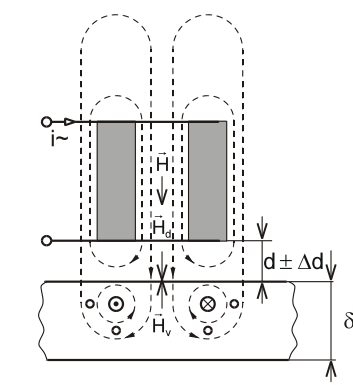
\includegraphics[width=0.5\linewidth]{figs/indukcnostni_senzor_virive_proudy.png}
    \caption{Indukčnostní senzor s vířivými proudy.}
    \label{fig:indukcnostni-senzor-s-virivymi-proudy}
\end{figure}
\end{tcolorbox}

\begin{tcolorbox}[title={\stepcounter{questionnumber}\thequestionnumber. Co měří a jak funguje senzor LVDT? (DT od slova differential transformer). Uveďte způsob vyhodnocení jeho výstupu. (24–26)}]
\textbf{LVDT} měří \textbf{lineární polohu}. Primární vinutí se budí AC signálem, dvě sekundární vinutí jsou zapojena diferenčně. Posun feromagnetického jádra zvýší vazbu na jedno sekundární vinutí a sníží na druhé.\\
Ve střední poloze je $U_2\approx0$, velikost výstupu odpovídá výchylce. \textbf{Fáze} určuje směr posuvu.\\
\textbf{Vyhodnocení:} synchronní detektor nebo rozdíl usměrněných sekundárních napětí; poměrové obvody AD598/AD698.
\begin{figure}[H]
    \centering
    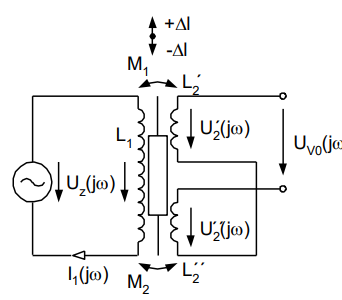
\includegraphics[width=0.5\linewidth]{figs/lvdt.png}
    \caption{Lineární diferenční transformátorový senzor polohy.}
    \label{fig:linearni-diferencni-transformatorovy-senzor-polohy}
\end{figure}
\end{tcolorbox}

% ---------------------------------------------------------% 7 — Měření lineární a úhlové polohy
% ---------------------------------------------------------

\newpage
\section*{7. Měření lineární a úhlové polohy – optoelektronické a ultrazvukové senzory}
\setcounter{chapternumber}{7}
\setcounter{questionnumber}{0}
% ---------------------------------------------------------

\begin{tcolorbox}[title={\stepcounter{questionnumber}\thequestionnumber. Jaké znáte senzory lineární polohy? Vyjmenujte základní principy a jeden popište podrobněji (obrázek). (3-9)}]
\textbf{Dvoustavové:} mikrospínač, jazýčkový kontakt, Wiegand, Hall/proximity.\\
\textbf{Spojité:} odporové, kapacitní, indukčnostní, LVDT, optické, ultrazvukové.\\
\textbf{Kódové:} inkrementální/absolutní, optické i magnetické.
\textbf{LVDT} 
\end{tcolorbox}

\begin{tcolorbox}[title={\stepcounter{questionnumber}\thequestionnumber. Jaké znáte senzory úhlové polohy? Vyjmenujte základní principy a jeden popište podrobněji (obrázek). (10)}]
\textbf{Odporové:} rotační potenciometr.\\
\textbf{Magnetické:} Hall/AMR/GMR + permanentní magnet, bezkontaktní potenciometr.\\
\textbf{Optické kódové:} inkrementální nebo absolutní kotouč + světelný paprsek.\\
\textbf{Indukční/transformátorové:} selsyn, induktosyn.
\end{tcolorbox}

\begin{tcolorbox}[title={\stepcounter{questionnumber}\thequestionnumber. Jaké znáte optické senzory vzdálenosti? Vyjmenujte základní principy a jeden popište podrobněji (obrázek). (13)}]
 \textbf{Intenzitní/reflexní} -- měří se \textbf{intenzita odraženého světla}.\\
  \textbf{Triangulační} -- se vzdáleností se mění \textbf{poloha dopadu paprsku} na detektoru.\\
  \textbf{ToF (Time of Flight)} -- měří se \textbf{doba letu} světla k objektu a zpět:
  \[
  l=\frac{ct}{2}
  \]
  \textbf{FMCW} -- vzdálenost se určí z \textbf{rozdílu frekvencí} vyslaného a odraženého signálu.\\
  \textbf{Interferenční} -- poloha se určí ze změny \textbf{interferenčního obrazce}.\\

  \textbf{Podrobně -- triangulační senzor:}\\
  Zdroj vyšle paprsek na objekt, odraz dopadá na \textbf{PSD/CMOS detektor}.
  Při změně vzdálenosti se mění \textbf{poloha světelné stopy} na detektoru.
  Výhoda oproti obyčejnému reflexnímu senzoru: menší závislost na \textbf{odrazivosti povrchu}.
\end{tcolorbox}

\begin{tcolorbox}[title={\stepcounter{questionnumber}\thequestionnumber. Jaký je rozdíl mezi inkrementálním a absolutním senzorem polohy, uveďte příklad od každého typu (obrázek, signály na výstupu). (19)}]
\textbf{Inkrementální} dává impulsy při pohybu => měří \textbf{změnu polohy}, po zapnutí nezná absolutní polohu. Směr se určí z \textbf{kvadraturních signálů A/B}. Příklad: optický rotační enkodér, digitální posuvka.

\textbf{Absolutní} dává přímo \textbf{kód polohy} => poloha je známá hned po zapnutí. Příklad: vícestopý optický enkodér s Grayovým kódem.

\begin{figure}[H]
    \centering
    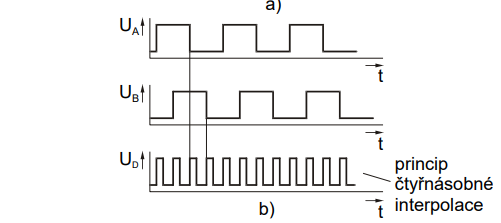
\includegraphics[width=0.55\linewidth]{figs/signaly.png}
    \caption{Kvadraturní signály A/B pro určení směru pohybu.}
    \label{fig:kvadraturni-signaly-a-b-pro-urceni-smeru-pohybu}
\end{figure}

\end{tcolorbox}


\begin{tcolorbox}[title={\stepcounter{questionnumber}\thequestionnumber. Na nakresleném schématu vysvětlete princip absolutního vícestopového snímače polohy. Jaký kód se v něm používá a proč? (23)}]

Používá se \textbf{Grayův kód} => mezi sousedními polohami se mění jen \textbf{1 bit}. Chyba při přechodu mezi dvěma polohami proto způsobí jen malou chybu, ne skok o mnoho bitů.

\begin{figure}[H]
    \centering
    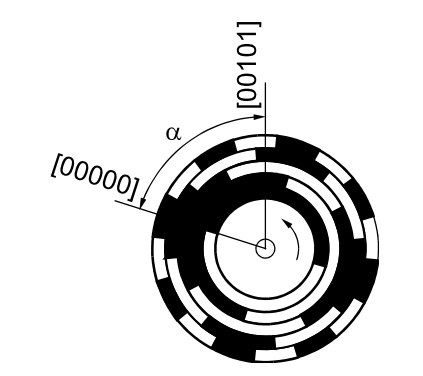
\includegraphics[width=0.55\linewidth]{figs/absolutni_vicestopy_encoder.png}
    \label{fig:abs-vicestop}
\end{figure}

\end{tcolorbox}


\begin{tcolorbox}[title={\stepcounter{questionnumber}\thequestionnumber. Na nakresleném schématu vysvětlete princip absolutního jednostopového snímače. Jaký kód se v něm používá a proč? (23)}]
Na jedné stopě je \textbf{cyklický pseudonáhodný kód}. Několik snímačů čte okno bitů vedle sebe; každé okno odpovídá jedné poloze.

\textbf{Výhoda:} absolutní poloha z jedné stopy.\\

\begin{figure}[H]
    \centering
    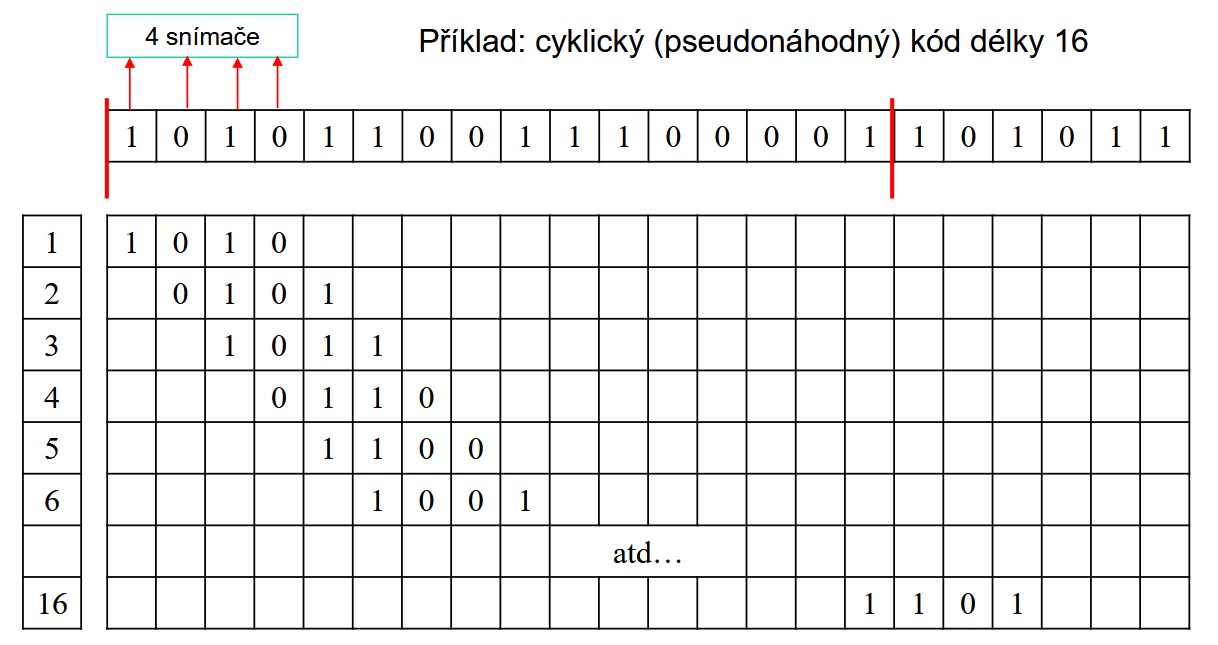
\includegraphics[width=\linewidth]{figs/jednostopy_inicializovany_encoder.png}
    \label{fig:jednostipy}
\end{figure}

\end{tcolorbox}


\begin{tcolorbox}[title={\stepcounter{questionnumber}\thequestionnumber. Popište princip senzorů vzdálenosti používajících frekvenční modulace. V jakých případech je tento princip vhodnější než přímé měření doby šíření pulzu? (27)}]
\textbf{FMCW:} vysílá se spojitý signál s lineárně měněnou frekvencí. Odražený signál je zpožděný, takže má proti aktuálně vysílanému signálu rozdíl frekvencí $\Delta f$.

\[
\Delta f \propto t \quad \Rightarrow \quad l=\frac{ct}{2}
\]

Vhodné, když je přímé měření krátkého času obtížné.
\end{tcolorbox}

\begin{tcolorbox}[title={\stepcounter{questionnumber}\thequestionnumber. Popište, jak fungují tři základní typy odrazných optických senzorů vzdálenosti. Jaké metody používají, aby odstranily vliv okolního světla a odrazivosti materiálu? (27)}]
\textbf{Difuzní reflexní:} vysílač i přijímač v jednom těle, přijímá se světlo rozptýlené od objektu.\\
\textbf{Retroreflexní:} světlo jde na odražeč a zpět; objekt paprsek přeruší, často se využívá \textbf{polarizace}.\\
\textbf{Triangulační:} vzdálenost se určí z polohy stopy na detektoru.

\textbf{Okolní světlo:} modulace vysílače + synchronní/pásmové vyhodnocení, optický filtr, odečtení signálu se zhasnutým zdrojem.\\
\textbf{Odrazivost/náklon:} triangulace nebo více přijímačů/senzorů pro kompenzaci.
\end{tcolorbox}

\begin{tcolorbox}[title={\stepcounter{questionnumber}\thequestionnumber. Uveďte tři způsoby, jak potlačit vliv okolního osvětlení na optický senzor polohy (zastínění se nepočítá). (27)}]
\textbf{Modulace světla} a synchronní detekce.\\
\textbf{Optický filtr} na vlnovou délku vysílače.\\
\textbf{Dvoufázové měření:} nejdřív okolní světlo, potom okolní světlo + zdroj => odečtení pozadí.
\end{tcolorbox}

\begin{tcolorbox}[title={\stepcounter{questionnumber}\thequestionnumber. Jak funguje triangulační senzor vzdálenosti – jakou má hlavní výhodu oproti obyčejnému reflexnímu? (29)}]
Poloha dopadu světla na detektoru se mění s vzdáleností objektu
\textbf{Výhoda oproti reflexnímu intenzitnímu senzoru:} vyhodnocuje se geometrie, ne jen intenzita => menší závislost na barvě a odrazivosti objektu.

\begin{figure}[H]
    \centering
    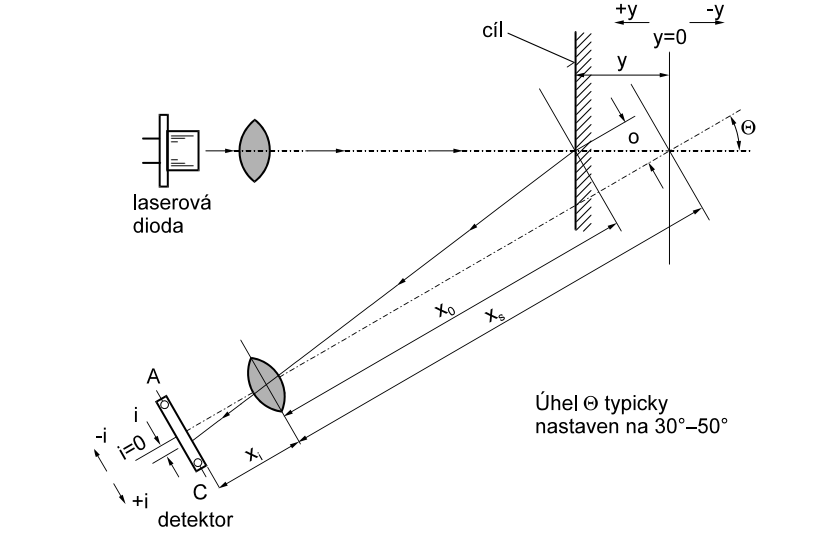
\includegraphics[width=0.55\linewidth]{figs/triangulacni_senzor.png}
    \label{fig:trian}
\end{figure}

\end{tcolorbox}


\begin{tcolorbox}[title={\stepcounter{questionnumber}\thequestionnumber. Popište princip senzorů vzdálenosti typu „Time of Flight“. V jakých případech se doslova vyhodnocuje čas, a kdy to technicky nejde? Jaká metoda se v takovém případě používá? (32)}]
\textbf{ToF} měří dobu letu signálu k objektu a zpět:
\[
l=\frac{ct}{2}
\]
\textbf{Přímý ToF:} větší vzdálenosti, TDC.\\
\textbf{Když přímý čas nejde měřit přesně:} používá se \textbf{indirect ToF} nebo \textbf{FMCW}.
\end{tcolorbox}

\begin{tcolorbox}[title={\stepcounter{questionnumber}\thequestionnumber. Na nakresleném schématu vysvětlete princip senzoru „Time of Flight“ s frekvenční modulací (FMCW). (32)}]
Vysílač mění frekvenci v čase. Odraz od objektu přijde se zpožděním $t$, proto má jinou frekvenci než právě vysílaný signál.

\[
\Delta f \propto t,\qquad l=\frac{ct}{2}
\]

\textbf{FMCW výhoda:} kromě vzdálenosti lze z Dopplerova posuvu určit i \textbf{rychlost}.
\end{tcolorbox}

\begin{tcolorbox}[title={\stepcounter{questionnumber}\thequestionnumber. Uveďte tři typy LiDARu bez pohyblivých součástí. Jaký princip používá LiDAR pro měření vzdálenosti? (35)}]
\textbf{Bez pohyblivých částí:} Flash LiDAR/RGBD kamera, optical phased array, fixed multi-beam LiDAR.

\textbf{Měření vzdálenosti:} hlavně \textbf{ToF} (přímý nebo nepřímý), případně \textbf{FMCW}. LiDAR = rychlý laserový dálkoměr/scanner.
\end{tcolorbox}

\begin{tcolorbox}[title={\stepcounter{questionnumber}\thequestionnumber. Jak funguje ultrazvukový dálkoměr? Napište rovnice. Uveďte tři možné příčiny chyb měření. (42)}]
\textbf{Piezoelektrický vysílač} vyšle ultrazvukový puls, přijímač detekuje odraz. Měří se doba letu:
\[
L=\frac{v t}{2}
\]
kde $v$ je rychlost zvuku.

\textbf{Chyby:} rychlost zvuku závisí na teplotě/vlhkosti/větru, špatný odraz nebo absorpce, mrtvá zóna po vyslání pulzu.
\end{tcolorbox}

\begin{tcolorbox}[title={\stepcounter{questionnumber}\thequestionnumber. Popište funkci ultrazvukového senzoru vzdálenosti (obrázek, rovnice, jak funguje vysílač/přijímač?). (42)}]
\textbf{Vysílač:} piezo měnič převede elektrický impuls na ultrazvuk.\\
\textbf{Přijímač:} piezo měnič převede odraženou vlnu zpět na napětí.\\
\textbf{Vyhodnocení:} ToF odrazu:
\[
L=\frac{v t}{2}
\]
Vysílač a přijímač mohou být oddělené nebo společné.
\end{tcolorbox}

\begin{tcolorbox}[title={\stepcounter{questionnumber}\thequestionnumber. Jaké jsou čtyři nevýhody ultrazvukového dálkoměru? Proč se vůbec používá? (42)}]
\textbf{Nevýhody:} závislost rychlosti zvuku na prostředí, \textbf{mrtvá zóna}, nutný kvalitní odraz, omezená rychlost měření/dosah.\\
\textbf{Proč se používá:} je \textbf{levný}, jednoduchý a nevadí mu barva ani průhlednost objektu tolik jako optice.
\end{tcolorbox}

\newpage
% ---------------------------------------------------------
% 8 — Senzory a převodníky pro měření rychlosti, zrychlení a vibrací
% ---------------------------------------------------------

\newpage
\section*{8. Senzory a převodníky pro měření rychlosti, zrychlení a vibrací}
\setcounter{chapternumber}{8}
\setcounter{questionnumber}{0}
% ---------------------------------------------------------

\begin{tcolorbox}[title={\stepcounter{questionnumber}\thequestionnumber. Jaké znáte senzory rychlosti (neúhlové)? Vyjmenujte základní principy a jeden popište podrobněji (obrázek). (2)}]
\textbf{Odvozené z polohy:} senzor polohy + derivace signálu:
\[
v=\frac{dx}{dt}
\]

\textbf{Elektrodynamické:} vodič/cívka se pohybuje v magnetickém poli => indukované napětí $u=Blv$.

\textbf{Elektromagnetické:} pohybuje se magnet nebo část magnetického obvodu vůči cívce => mění se magnetický tok:
\[
u=-N\frac{d\Phi}{dt}
\]

\textbf{Korelační:} dva senzory ve vzdálenosti $\Delta x$ snímají stejný náhodný obraz povrchu. Maximum korelace dá zpoždění $\tau_{\max}$:
\[
v=\frac{\Delta x}{\tau_{\max}}
\]

\textbf{Dopplerovské:} radar/LiDAR/ultrazvuk vysílá vlnění, odražený signál má \textbf{frekvenční posuv} úměrný rychlosti objektu.
\end{tcolorbox}

\begin{tcolorbox}[title={\stepcounter{questionnumber}\thequestionnumber. Na nakresleném schématu vysvětlete princip elektrodynamického senzoru rychlosti a napište rovnici pro jeho výstupní napětí. (3)}]
\textbf{Princip:} vodič/cívka se pohybuje rychlostí $v$ v magnetickém poli $B$. Vodič protíná magnetické indukční čáry => indukuje se napětí úměrné rychlosti:
\[
u=Blv
\]
Pro cívku se více závity se napětí násobí počtem aktivních vodičů.

\begin{figure}[H]
    \centering
    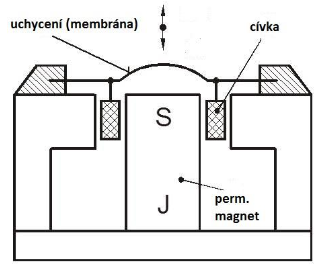
\includegraphics[width=0.5\linewidth]{figs/elektrodynamicky_senzor_rychlosti.png}
    \caption{Elektrodynamický senzor rychlosti.}
    \label{fig:elektrodynamicky-senzor-rychlosti}
\end{figure}

\end{tcolorbox}


\begin{tcolorbox}[title={\stepcounter{questionnumber}\thequestionnumber. Jaké znáte senzory úhlové rychlosti? Vyjmenujte základní principy a jeden popište podrobněji (obrázek). (4–5, 8–14)}]
\textbf{Tachogenerátor DC:} napětí úměrné $\omega$, umí indikovat směr, ale má komutátor.\\
\textbf{Tachoalternátor AC:} střídavý výstup, frekvence/amplituda souvisí s otáčkami, bez kartáčů.\\
\textbf{Detekce značek:} indukční, Wiegand, dvoustavové, vířivoproudé, optické => z impulsů se určí otáčky.\\
\textbf{MEMS gyroskop:} Coriolisova síla na kmitající hmotu.\\
\textbf{FOG:} optický vláknový gyroskop, \textbf{Sagnacův jev}.

\textbf{Podrobně tachogenerátor:}
\[
U=2NhrB\omega,\qquad \omega=\frac{2\pi n}{60}
\]
\end{tcolorbox}

\begin{tcolorbox}[title={\stepcounter{questionnumber}\thequestionnumber. Princip dvou typů senzoru úhlové rychlosti (obrázek, popis). (4–5, 8–14)}]
\textbf{1) Tachogenerátor:} konstrukčně podobný točivému stroji. Výstupní napětí je úměrné úhlové rychlosti:
\[
U=2NhrB\omega
\]
\textbf{DC tachodynamo} má komutátor a umožní směr otáčení, \textbf{AC tachoalternátor} je bezkartáčový.

\textbf{2) Detekce značek:} značka na hřídeli prochází kolem senzoru => vznikají impulsy. Z frekvence impulsů se určí otáčky:
\[
\omega=\frac{2\pi n}{60}
\]
Používá se \textbf{indukční}, \textbf{Wiegandův}, \textbf{optoelektronický} nebo \textbf{vířivoproudý} senzor.

\begin{figure}[H]
\centering
\begin{minipage}{0.48\linewidth}
    \centering
    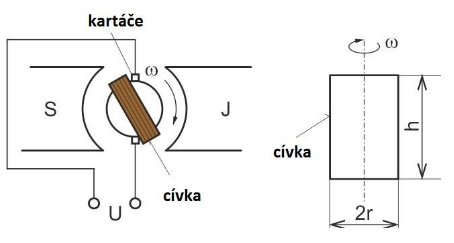
\includegraphics[width=\linewidth]{figs/tachodynamo.png}
    \caption{Tachodynamo.}
    \label{fig:tachodynamo}
\end{minipage}
\hfill
\begin{minipage}{0.48\linewidth}
    \centering
    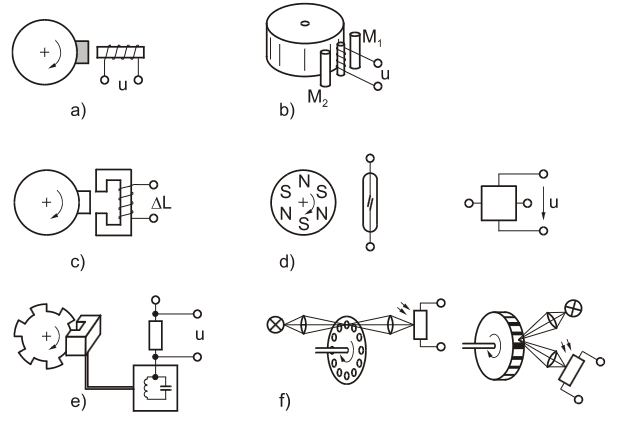
\includegraphics[width=\linewidth]{figs/senzory_uhlove_rychlosti.png}
    \caption{Senzory úhlové rychlosti.}
    \label{fig:senzory-uhlove-rychlosti}
\end{minipage}
\end{figure}


\end{tcolorbox}


\begin{tcolorbox}[title={\stepcounter{questionnumber}\thequestionnumber. Na nakresleném schématu vysvětlete princip senzoru úhlové rychlosti na principu Coriolisovy síly v MEMS provedení a napište rovnici, na které je založen. (0)}]
\textbf{Princip:} v MEMS gyroskopu kmitá malá hmota rychlostí $\vec v$. Při rotaci působí \textbf{Coriolisova síla} kolmo na směr kmitání:
\[
\vec F_C=-2m\vec\omega\times \vec v
\]
Boční výchylka se měří typicky \textbf{kapacitně} => výstup je úměrný $\omega$.

\begin{figure}[H]
    \centering
    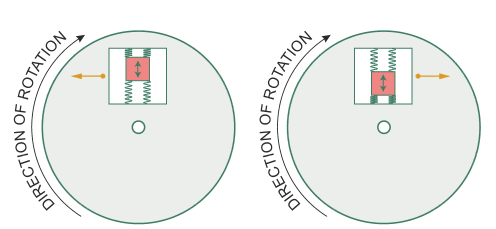
\includegraphics[width=0.5\linewidth]{figs/mems_coriolisuv_gyroskop.png}
    \caption{Gyroskopy na principu Coriolisovy síly (MEMS).}
    \label{fig:gyroskopy-na-principu-coriolisovy-sily-mems}
\end{figure}

\end{tcolorbox}


\begin{tcolorbox}[title={\stepcounter{questionnumber}\thequestionnumber. Na nakresleném schématu vysvětlete princip mikromechanického akcelerometru používaného pro navigaci. (16)}]
\textbf{MEMS kapacitní akcelerometr:} seismická hmota je zavěšená na pružných tětivách. Zrychlení vychýlí hmotu => změní se \textbf{diferenciální kapacity} hřebínkových elektrod.

\[
F=ma=kx
\]

\textbf{Výstup:} změna kapacity $\Delta C$ odpovídá zrychlení.

\begin{figure}[H]
    \centering
    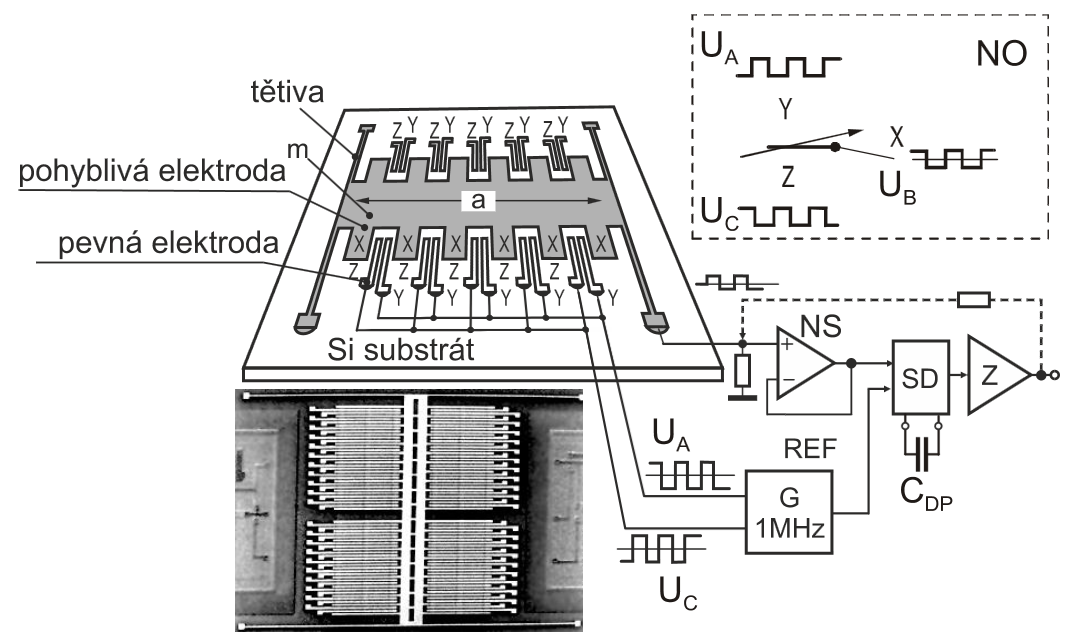
\includegraphics[width=0.7\linewidth]{figs/mems_kapacitni_akcelerometr.png}
    \caption{MEMS kapacitní akcelerometr.}
    \label{fig:mems-kapacitni-akcelerometr}
\end{figure}

\end{tcolorbox}


\begin{tcolorbox}[title={\stepcounter{questionnumber}\thequestionnumber. Jaký je princip akcelerometru, který dokáže měřit konstantní zrychlení, např. tíhové zrychlení? (15–17)}]
Musí umět měřit \textbf{statické vychýlení seismické hmoty}. Proto se hodí \textbf{kapacitní MEMS} nebo \textbf{servoakcelerometr}.

\textbf{Servoakcelerometr:} zpětná vazba drží hmotu v nulové poloze. Měřený proud v cívce vytváří kompenzační sílu => proud je úměrný zrychlení.

\begin{figure}[H]
    \centering
    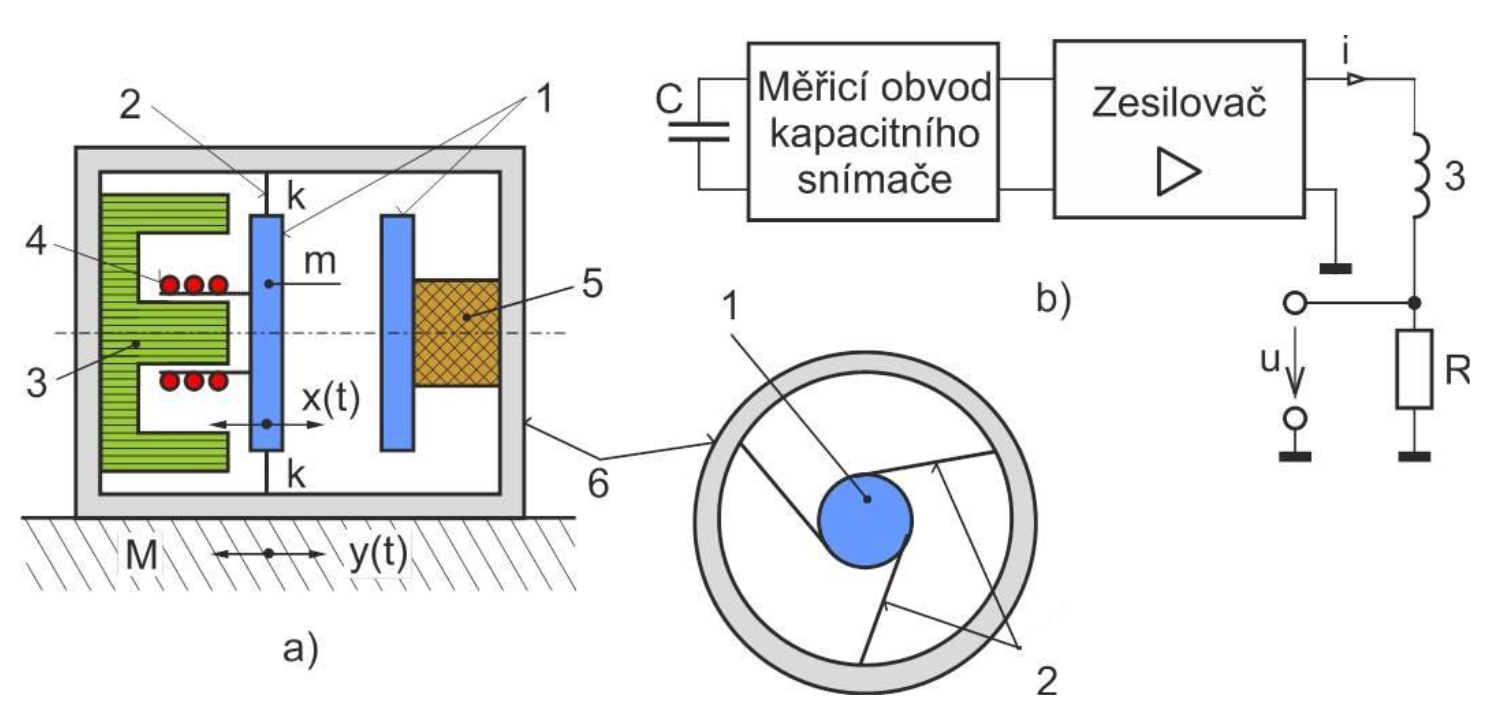
\includegraphics[width=0.75\linewidth]{figs/zpetnovazebni_kapacitni_akcelerometr.png}
    \caption{Zpětnovazební kapacitní akcelerometr.}
    \label{fig:zpetnovazebni-kapacitni-akcelerometr}
\end{figure}

\end{tcolorbox}


\begin{tcolorbox}[title={\stepcounter{questionnumber}\thequestionnumber. Jak se dá měřit statické zrychlení (například vektor gravitace)? (16–17)}]
\textbf{Kapacitním MEMS akcelerometrem:} tíhové zrychlení vychýlí seismickou hmotu.
\[
F=ma=kx
\]
Výchylka $x$ se převede na \textbf{změnu kapacity}. Podle složek zrychlení lze určit směr vektoru gravitace.
\end{tcolorbox}

\begin{tcolorbox}[title={\stepcounter{questionnumber}\thequestionnumber. Jak se liší absolutní a relativní senzor vibrací? Vysvětlete základní princip. (18)}]
\textbf{Relativní senzor:} měří pohyb vůči vnějšímu vztažnému bodu, typicky senzor polohy nebo laserový vibrometr.\\
\textbf{Absolutní senzor:} má vztažný bod uvnitř senzoru = \textbf{seismická hmota}. Měří se relativní pohyb hmoty vůči pouzdru.
\end{tcolorbox}

\begin{tcolorbox}[title={\stepcounter{questionnumber}\thequestionnumber. Popište princip senzoru vibrací – akcelerometru (jeden nebo více typů). (18–23)}]
\textbf{Absolutní senzor vibrací:} pouzdro sleduje kmitající objekt, seismická hmota má setrvačnost. Měří se její relativní výchylka $x$.

\[
m\frac{d^2x}{dt^2}+b\frac{dx}{dt}+kx=-m\frac{d^2y}{dt^2}
\]

\textbf{Piezoelektrický akcelerometr:} zrychlení působí silou na piezoelement => vzniká náboj. Má vysokou rezonanční frekvenci, ale \textbf{neměří DC}.\\
\textbf{Elektrodynamický rychloměr:} cívka jako seismická hmota, výstup $u=Blv$ je úměrný rychlosti.

\begin{figure}[H]
    \centering
    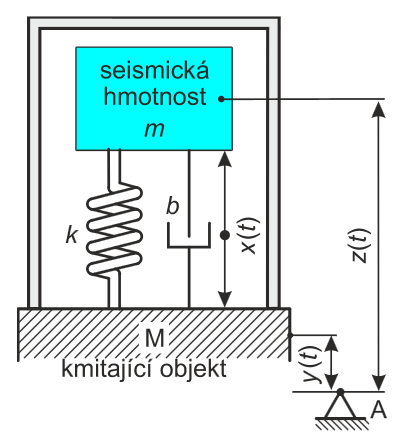
\includegraphics[width=0.5\linewidth]{figs/kmitajici_objekt.png}
    \caption{Kmitající objekt.}
    \label{fig:kmitajici-objekt}
\end{figure}

\begin{figure}[H]
    \centering
    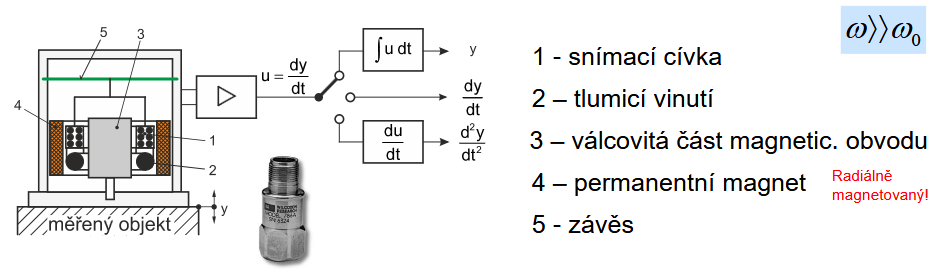
\includegraphics[width=1\linewidth]{figs/piezoelektricky_snimac_vibraci.png}
    \label{fig:rychlomer}
\end{figure}

\end{tcolorbox}

\begin{tcolorbox}[title={\stepcounter{questionnumber}\thequestionnumber. V jakých dvou módech může pracovat senzor kmitavého pohybu (v čem se liší)? (20–21)}]
\textbf{1) Akcelerometrický mód:}
\[
\omega \ll \omega_0
\]
Výchylka seismické hmoty je úměrná \textbf{zrychlení}:
\[
x(t)\approx -\frac{1}{\omega_0^2}a(t)
\]

\textbf{2) Mód měření amplitudy/výchylky:}
\[
\omega \gg \omega_0
\]
Seismická hmota je téměř v klidu v inerciální soustavě, relativní pohyb odpovídá \textbf{výchylce objektu}:
\[
x(t) \approx -y(t)
\]
\end{tcolorbox}

\begin{tcolorbox}[title={\stepcounter{questionnumber}\thequestionnumber. Jak se dá zpracovat signál z piezoelektrického senzoru síly nebo zrychlení (schéma, popis). (23)}]
\textbf{Piezoelektrický senzor} generuje náboj $Q$ úměrný síle/zrychlení. Signál se zpracuje \textbf{nábojovým zesilovačem}: operační zesilovač s kapacitou $C_i$ ve zpětné vazbě převede náboj na napětí.
\[
U_{\text{out}}\approx -\frac{Q}{C_i}
\]
\textbf{Nevýhoda:} kvůli svodům neměří \textbf{stejnosměrně} ani velmi pomalé změny.

\begin{figure}[H]
    \centering
    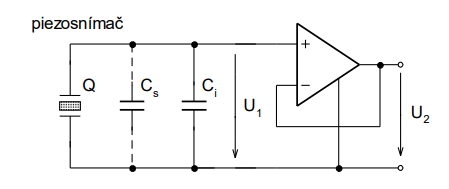
\includegraphics[width=0.5\linewidth]{figs/piezzosnimac.png}
    \caption{Zpracovaní signálu z piezoel. senzoru, $C_s$ - parazitní.}
    \label{fig:zpracovani-signalu-z-piezoel-senzoru-c-s-parazitni}
\end{figure}
\end{tcolorbox}



% ---------------------------------------------------------
% 9 — Měření teploty
% ---------------------------------------------------------

\newpage
\section*{9. Měření teploty}
\setcounter{chapternumber}{9}
\setcounter{questionnumber}{0}
% ---------------------------------------------------------

\begin{tcolorbox}[title={\stepcounter{questionnumber}\thequestionnumber. Jaké znáte kontaktní senzory pro měření teploty, který byste použili pro běžné měření teploty místnosti – proč? (3)}]
\textbf{RTD kovové} -- Pt100/Pt1000.\\
\textbf{Termistory} -- NTC/PTC.\\
\textbf{PN polovodičové senzory}.\\
\textbf{Integrované digitální senzory}.\\
\textbf{Termočlánky}.

\textbf{Na běžnou místnost:} \textbf{NTC} nebo \textbf{integrovaný digitální senzor} => dobrá citlivost a jednoduché vyhodnocení v malém rozsahu.
\end{tcolorbox}

\begin{examplebox}[title={NTC termistor – určení konstanty B}]
\textbf{Otázka:} Pro NTC termistor s charakteristikou $R=Ae^{B/T}$ odvoďte vztah pro výpočet konstanty $B$ ze dvou měření odporu při teplotách $T_1$ a $T_2$. Uveďte, jak se odpor mění s teplotou a kde se NTC termistory typicky používají.\\
\textbf{Odpověď:}
\[
R=Ae^{B/T}
\]
\[
\ln R=\ln A+\frac{B}{T}
\]
\[
B=\frac{\ln(R_1/R_2)}{1/T_1-1/T_2}
\]
\textbf{NTC:} s rostoucí teplotou odpor \textbf{klesá}. Použití: běžné kontaktní měření teploty, kompenzace, ochrany, hlídání teploty elektroniky.
\end{examplebox}

\begin{tcolorbox}[title={\stepcounter{questionnumber}\thequestionnumber. Popište funkci polovodičového senzoru teploty (kontaktního, včetně nejjednoduššího zapojení pro měření). (6–10)}]
\textbf{Princip:} PN přechod v propustném směru je napájen \textbf{konstantním proudem}. Napětí na přechodu klesá s teplotou cca \textbf{$-2$ až $-2{,}3$ mV/K}.
\[
U_NP=mU_T\ln\left(\frac{I_D}{I_S}+1\right)
\]

\textbf{Nejjednodušší zapojení:} zdroj konstantního proudu + tranzistorová dioda. Nevýhoda dvouvodičově => odpor přívodů způsobuje chybu.
\begin{figure}[H]
    \centering
    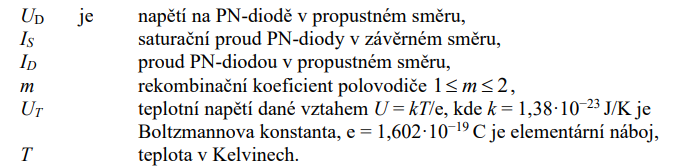
\includegraphics[width=0.5\linewidth]{figs/pn_prechod_teplotni_zavislost.png}
    \label{fig:udpn}
\end{figure}
\begin{figure}[H]
    \centering
    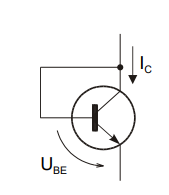
\includegraphics[width=0.2\linewidth]{figs/tranzdioda.png}
    \caption{Tranzistorová dioda.}
    \label{fig:tranzistorova-dioda}
\end{figure}
\begin{figure}[H]
    \centering
    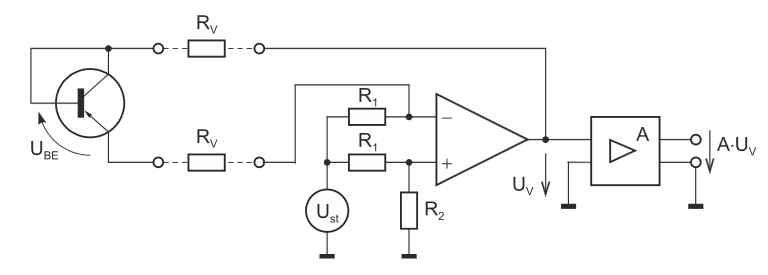
\includegraphics[width=0.2\linewidth]{figs/polovodicovy_senzor_teploty_schema.png}
    \caption{Zapojení polovodičového senzoru teploty.}
    \label{fig:zapojeni-polovodicoveho-senzoru-teploty}
\end{figure}
\end{tcolorbox}

\begin{examplebox}[title={Polovodičový senzor teploty – tranzistorová dioda}]
\textbf{Otázka:} Pro polovodičový senzor teploty s tranzistorovou diodou odvoďte vztah mezi proudem $I_D$ a napětím $U_D$. Vysvětlete, proč je teplotní koeficient napětí na PN přechodu přibližně $-2$ až $-2{,}3$~mV/K.\\
\textbf{Odpověď:}
\[
I_D=I_S\left(e^{U_D/(mU_T)}-1\right)
\]
Pro $I_D\gg I_S$:
\[
U_D=mU_T\ln\left(\frac{I_D}{I_S}\right)
\]
Při konstantním proudu se s rostoucí teplotou mění $U_T$ i $I_S$; výsledkem je přibližně:
\[
\left(\frac{\partial U_D}{\partial T}\right)_{I_D}\approx -2\ \text{až}\ -2{,}3\ \mathrm{mV/K}
\]
\textbf{Tranzistorová dioda:} tranzistor se zapojí jako dioda, typicky $m\approx1$.
\end{examplebox}

\begin{examplebox}[title={Polovodičový senzor teploty – aktivní můstek}]
\textbf{Otázka:} Pro zapojení polovodičového senzoru teploty v aktivním můstku určete vztah pro výstupní napětí. Navrhněte hodnoty prvků tak, aby zesílené výstupní napětí v mV přímo odpovídalo teplotě ve stupních Celsia.\\
\textbf{Odpověď:}
\textbf{Cíl zapojení:} odečíst napěťový offset PN přechodu a zesílit teplotní změnu. PN přechod má citlivost přibližně:
\[
\Delta U_D \approx -2\ \mathrm{mV/K}\cdot \Delta T
\]
Zesílením s vhodným znaménkem lze nastavit např. \textbf{10 mV/$^\circ$C} jako u LM35. Integrované senzory řeší i závislost $I_S$ pomocí rozdílu napětí dvou tranzistorů:
\[
\Delta U_{BE}=U_T\ln r=\frac{kT}{e}\ln r
\]
=> napětí je přímo úměrné \textbf{absolutní teplotě}.
\end{examplebox}

\begin{tcolorbox}[title={\stepcounter{questionnumber}\thequestionnumber. Jak funguje bezkontaktní teploměr – pyrometr? (14–17)}]
\textbf{Pyrometr} měří \textbf{tepelné IR záření} vyzařované povrchem tělesa. Optika soustředí záření na IR detektor => ohřeje se a vygeneruje slabé napětí, elektronika z intenzity záření určí teplotu.

\[
M_0=\sigma T^4
\]
Reálný povrch:
\[
M=\varepsilon\sigma T^4
\]
Měří se tedy hlavně \textbf{povrchová teplota} a výsledek závisí na \textbf{emisivitě}.
\end{tcolorbox}

\begin{tcolorbox}[title={\stepcounter{questionnumber}\thequestionnumber. Jaké jsou výhody a nevýhody bezkontaktního měření teploty? (14–15)}]
\textbf{Výhody:} neovlivňuje objekt, měří pohybující se/rotující tělesa, rychlé změny, termovize zobrazí celé povrchy.\\
\textbf{Nevýhody:} chyba \textbf{emisivity}, chyba \textbf{prostupnosti prostředí}, vliv \textbf{odraženého záření}, měří jen \textbf{povrch}.
\end{tcolorbox}

\begin{tcolorbox}[title={\stepcounter{questionnumber}\thequestionnumber. Co omezuje přesnost bezkontaktního senzoru teploty? Jak se tyto chyby dají potlačovat? (14–20)}]
\textbf{Emisivita $\varepsilon$:} nastavit podle materiálu, použít štítek/barvu se známou emisivitou, ověřit kontaktním čidlem.\\
\textbf{Odražené záření okolí:} zadat zdánlivou odraženou teplotu, měřit vhodným úhlem.\\
\textbf{Prostupnost prostředí:} zohlednit atmosféru, kouř, páru, okna; obyčejné sklo IR často nepropouští.\\
\textbf{Geometrie:} měřený objekt musí vyplnit zorné pole.
\end{tcolorbox}

\begin{tcolorbox}[title={\stepcounter{questionnumber}\thequestionnumber. Co je to emisivita, jak se uplatňuje při měření? (popis, příklad, rovnice) (18–20)}]
\textbf{Emisivita $\varepsilon$} = poměr vyzařování reálného tělesa k černému tělesu:
\[
\varepsilon=\frac{M}{M_0}
\]
\[
M=\varepsilon\sigma T^4
\]
Při špatně nastavené $\varepsilon$ pyrometr spočítá špatnou \textbf{skutečnou teplotu}. Emisivita závisí na materiálu, vlnové délce, teplotě a úhlu.
\end{tcolorbox}



\begin{tcolorbox}[title={\stepcounter{questionnumber}\thequestionnumber. Jaké znáte senzory infračerveného záření (vyjmenujte, jeden popište podrobněji). (21–28)}]
\textbf{Termočlánková baterie / thermopile:} IR ohřeje absorpční plochu, termočlánky vytvoří napětí.\\
\textbf{Bolometr:} IR ohřeje odporový element => změní se odpor.\\
\textbf{Pyroelektrický detektor:} změna teploty změní spontánní polarizaci => vznikne náboj.\\
\textbf{Kvantový detektor / IR fotodioda:} fotony generují nosiče náboje v polovodiči.

\textbf{Podrobně bolometr:} pixel je tenká membrána s odporovou vrstvou. IR záření ji ohřeje, odpor se změní a CMOS elektronika změnu vyhodnotí. V termokamerách tvoří matici \textbf{FPA}.
\end{tcolorbox}

\begin{tcolorbox}[title={\stepcounter{questionnumber}\thequestionnumber. Uveďte dva základní principy, na kterých pracují pixelové senzory moderních pyrokamer s velkým rozlišením. Jaké jsou jejich hlavní výhody a nevýhody? U kterého z nich se používá chlazení senzoru a proč? (24–28)}]
\textbf{1) Mikrobolometry:} IR ohřeje membránu pixelu => změní se odpor.\\
\textbf{Výhody:} nevyžadují chlazení, levnější, vhodné pro běžné termokamery.\\
\textbf{Nevýhody:} pomalejší a méně citlivé než kvantové.

\textbf{2) Kvantové detektory:} IR foton excituje nosiče v polovodiči.\\
\textbf{Výhody:} velmi rychlé a citlivé.\\
\textbf{Nevýhody:} vyžadují \textbf{chlazení}, protože musí operovat při malých teplotách (aby nebyly nosiče už excitovány).
\end{tcolorbox}

\begin{tcolorbox}[title={\stepcounter{questionnumber}\thequestionnumber. Jaká je základní nevýhoda pyroelektrického senzoru teploty a proč a kde se vůbec používá? (26–27)}]
\textbf{Nevýhoda:} reaguje jen na \textbf{změnu teploty/záření}, ne na konstantní záření.\\
\textbf{Proč:} pyroelektrický jev = změna spontánní polarizace při změně $T$.\\
\textbf{Řešení:} rotující clona/chopper nebo pohyb objektu => uměle se vytvoří střídavý signál.\\
\textbf{Použití:} PIR detektory pohybu osob, detekce plamene, plynové analyzátory.
\end{tcolorbox}

\begin{tcolorbox}[title={\stepcounter{questionnumber}\thequestionnumber. Pro který typ pyrometru má neznalost emisivity měřeného objektu menší vliv na přesnost měření teploty? Naznačte, jak se to odvodí. Jakou nevýhodou je to vykoupeno? (30–31)}]
\textbf{Menší vliv má poměrový / dvoupásmový pyrometr.} Měří signál ve dvou vlnových délkách a vyhodnocuje jejich poměr.

Když je emisivita v obou pásmech přibližně stejná, pak se v poměru \textbf{vykrátí}. Teplota se určí hlavně z tvaru spektra.

\begin{figure}[H]
    \centering
    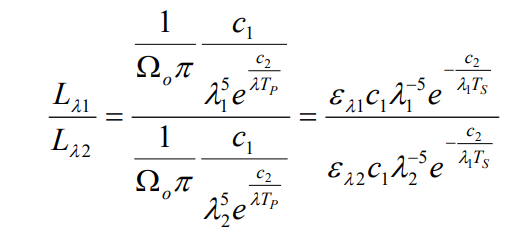
\includegraphics[width=0.5\linewidth]{figs/pyrometr_pomerove_mereni.png}
    \caption{Odvození.}
    \label{fig:odvozeni}
\end{figure}

\textbf{Nevýhody:} složitější optika/elektronika, dva detekční kanály, předpoklad stejné emisivity nemusí platit.
\end{tcolorbox}

% ---------------------------------------------------------
% 10 — Měření síly, tlaku, hladiny a průtoku
% ---------------------------------------------------------

\newpage
\section*{10. Měření síly, tlaku hladiny a průtoku}
\setcounter{chapternumber}{10}
\setcounter{questionnumber}{0}
% ---------------------------------------------------------

\begin{tcolorbox}[title={\stepcounter{questionnumber}\thequestionnumber. Jak se dá zpracovat signál z piezoelektrického senzoru síly nebo zrychlení (schéma, popis) (15–18)}]
\textbf{Piezoelektrický senzor} je zdroj náboje $Q$ s vlastní kapacitou. Problém napěťového zesilovače: výstup závisí na \textbf{kapacitě kabelu}.\\
\textbf{Řešení: nábojový zesilovač} -- OZ s kapacitou $C_f$ ve zpětné vazbě:
\[
U_{\text{out}} = -\frac{Q}{C_f}
\]
\textbf{Výhoda:} nezávisí na kapacitě kabelu, vstup je ve \textbf{virtuální zemi}.\\
\textbf{Nevýhoda piezo senzoru:} neumí měřit \textbf{statické veličiny}; náboj se vybíjí přes $R_g$:
\[
\tau = R_g C_f
\]
\begin{figure}[H]
    \centering
    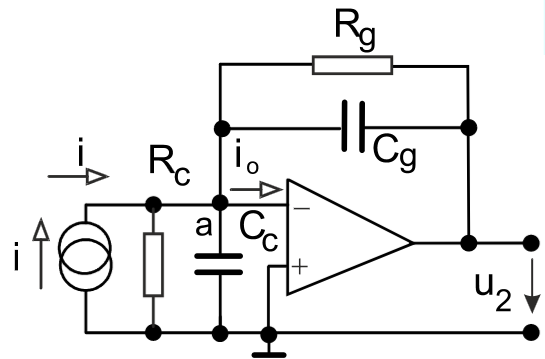
\includegraphics[width=0.4\linewidth]{figs/nabojovy_zesilovac.png}
    \caption{Nabojový zesilovač.}
    \label{fig:nabojovy-zesilovac}
\end{figure}
\end{tcolorbox}

\begin{tcolorbox}[title={\stepcounter{questionnumber}\thequestionnumber. Jak se dá měřit krouticí moment? Nakreslete a popište podrobněji nějaký princip. (22–29)}]
\textbf{Principy:} tenzometry na torzně namáhaném členu, měření \textbf{úhlového zkrutu}, magnetoelastický/magnetoanizotropní princip.

\textbf{1) Tenzometry:} krouticí moment způsobí smykovou deformaci hřídele/pružného členu. Tenzometry v můstku převedou deformaci na napětí.
\begin{figure}[H]
\centering
\begin{minipage}{0.25\linewidth}
\[
\gamma = \frac{M r}{GJ}, \qquad \varphi = \frac{M L}{GJ}
\]
\end{minipage}
\hfill
\begin{minipage}{0.70\linewidth}
    \centering
    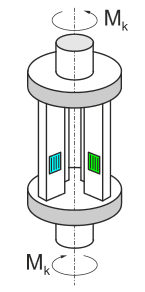
\includegraphics[width=0.13\linewidth]{figs/krizovy_pruzny_clen.png}
    \caption{Krizový pružný člen.}
    \label{fig:krizovy-pruzny-clen}
\end{minipage}
\end{figure}




\medskip
\textbf{2) Převod momentu na úhel:} na hřídeli jsou dvě značky ve vzdálenosti $L$. Moment způsobí \textbf{zkrut} $\Theta$, který se snímá opticky/indukčně/Hallově.
\begin{figure}[H]
\centering
\begin{minipage}{0.25\linewidth}
\[
M = GJ \frac{\varphi}{L}
\]
\end{minipage}
\hfill
\begin{minipage}{0.70\linewidth}

    \centering
    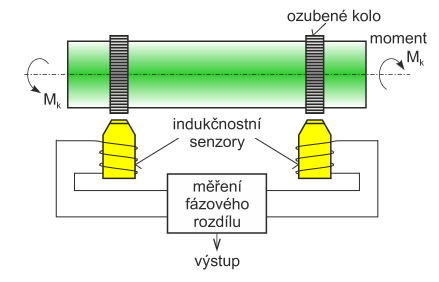
\includegraphics[width=0.6\linewidth]{figs/kroutici_moment_uhlova_deformace.png}
    \caption{Sensor krouticího momentu.}
    \label{fig:sensor-krouticiho-momentu}
\end{minipage}

\end{figure}


\medskip
\textbf{3) Magnetické senzory momentu:} krouticí moment mění \textbf{permeabilitu} nebo rozložení magnetického pole v materiálu. Výstup fluxgate/Hall senzorů => moment.
\begin{figure}[H]
    \centering
    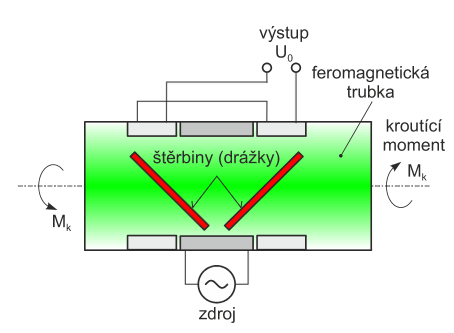
\includegraphics[width=0.4\linewidth]{figs/magneticky_senzor_krouticiho_momentu.png}
    \caption{Magnetický senzor momentu.}
    \label{fig:magneticky-senzor-momentu}
\end{figure}

\end{tcolorbox}

\begin{tcolorbox}[title={\stepcounter{questionnumber}\thequestionnumber. Jaké znáte senzory tlaku plynu? (druhy, na základě čeho se tlak obvykle měří, jak se to vyhodnocuje?) (31–41)}]
\textbf{Tlak:} $p=\frac{dF}{dS}$. Obvykle se převede na \textbf{sílu/deformaci pružného členu} a ta na elektrický signál.

\textbf{Membránové s tenzometry:} tlak deformuje membránu => změna odporu tenzometrů v můstku.\\
\textbf{Trubicové deformační:} Bourdonova trubice, tlak mění tvar/polohu.\\
\textbf{Kapacitní MEMS:} membrána tvoří elektrodu diferenčního kapacitoru => změna $C$.\\
\textbf{Piezoelektrické:} tlak vyvolá náboj, vhodné hlavně pro \textbf{rychlé změny tlaku}.\\
\textbf{Resonanční:} tlak mění napětí rezonátoru => změna rezonanční frekvence.

\textbf{Vyhodnocení:} změna \textbf{odporu}, \textbf{kapacity}, \textbf{náboje} nebo \textbf{frekvence}.
\end{tcolorbox}

\begin{tcolorbox}[title={\stepcounter{questionnumber}\thequestionnumber. Uveďte základní typy průtokoměrů. Které se hodí na měření průtoku vzduchu v klimatizační technice? (46–49)}]
\textbf{Objemové:} dávkovací, plováčkové/rotametr, rychlostní.\\
\textbf{Rychlostní:} turbínkové, vírové, indukční, ultrazvukové, škrticí orgány, značkovací.\\
\textbf{Hmotnostní:} Coriolisovy, tepelné/kalorimetrické.

\textbf{Pro klimatizační techniku (vzduch):}  
vhodné jsou hlavně \textbf{tepelné anemometry} a \textbf{ultrazvukové} průtokoměry.
\end{tcolorbox}

\begin{tcolorbox}[title={\stepcounter{questionnumber}\thequestionnumber. Jak se dá změřit hmotnostní průtok (popis, obrázek, rovnice)? (48–49)}]
\textbf{Hmotnostní průtok:}
\[
Q_m = \frac{m}{t}
\]

\textbf{1) Coriolisův průtokoměr:} trubice se rozkmitá, proudící kapalina vyvolá \textbf{Coriolisovu sílu} a zkroucení/fázový posun kmitů. Měří přímo $Q_m$.
\[
\Delta F_C=2w\omega\Delta m
=2\frac{\Delta l}{\Delta t}\omega\Delta m
=2Q_m\omega\Delta l
\]

\begin{figure}[H]\centering
    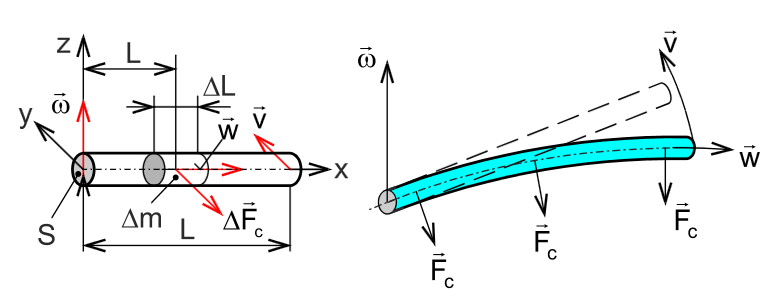
\includegraphics[width=0.5\linewidth]{figs/coriolisuv_prutokomer.png}
    \caption{Coriolisův průtokoměr}
    \label{fig:coriolisuv-prutokomer}
\end{figure}

\textbf{2) Tepelné průtokoměry:} ohřátý senzor je ochlazován prouděním. U diferenčního termoanemometru se při $v=0$ teploty senzorů rovnají, při proudění se jeden ochladí a druhý ohřeje. Vhodné hlavně pro \textbf{plyny a malé průtoky}.

\begin{figure}[H]
    \centering
    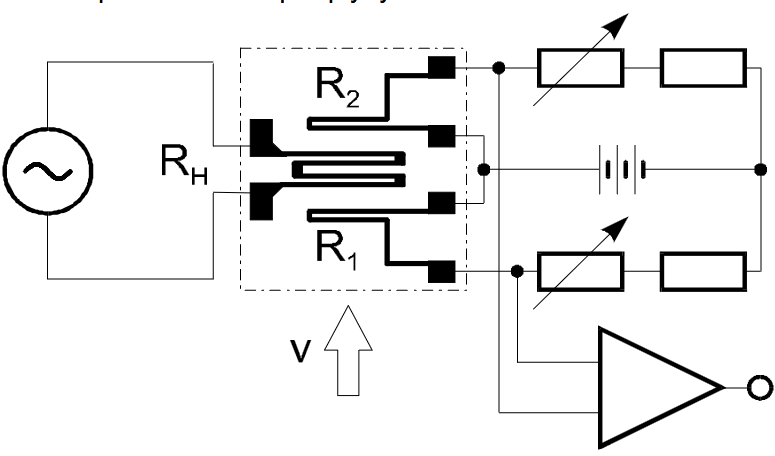
\includegraphics[width=0.5\linewidth]{figs/tepelny_prutokomer.png}
    \caption{Tepelné sensory hmotnostního průtoku}
    \label{fig:tepelne-sensory-hmotnostniho-prutoku}
\end{figure}
\end{tcolorbox}

\begin{tcolorbox}[title={\stepcounter{questionnumber}\thequestionnumber. Jak funguje indukční průtokoměr? (rovnice, obrázek, popis) (54–55)}]
\textbf{Princip:} vodivá kapalina proudí rychlostí $v$ v magnetickém poli $B$. Náboj v kapalině je vychýlen Lorentzovou silou, na elektrodách vzniká napětí:
\[
U = B \, D \, v,
\]
kde $D$ je průměr trubice. Protože $Q_v=vS$, napětí je úměrné \textbf{objemovému průtoku}.\\
\textbf{Podmínka:} kapalina musí být \textbf{vodivá}. Napětí je malé => používá se střídavé $B$.

\begin{figure}[H]
    \centering 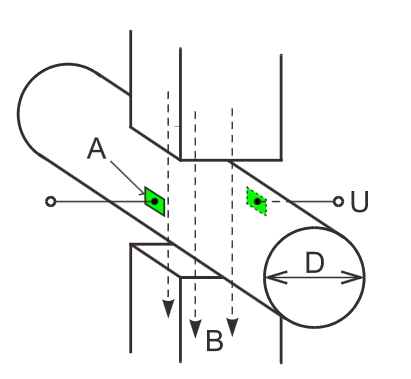
\includegraphics[width=0.2\linewidth]{figs/indukcni_prutokomer.png}
    \caption{Indukční průtokoměr}
    \label{fig:indukcni-prutokomer}
\end{figure}
\end{tcolorbox}

\begin{tcolorbox}[title={\stepcounter{questionnumber}\thequestionnumber. Popište funkci ultrazvukového průtokoměru. (52–53)}]
\textbf{Transit-time princip:} ultrazvukový puls se šíří jednou po proudu a jednou proti proudu. Skládá se rychlost zvuku $c$ a rychlost proudění $w$.
\[
t_1 = \frac{L}{c - w \cos\alpha}, \qquad
t_2 = \frac{L}{c + w \cos\alpha},
\]
kde $L$ je délka dráhy a $\alpha$ úhel vůči směru proudění. Z rozdílu časů:
\[
w = \frac{L}{2 \cos\alpha} \cdot \frac{t_2 - t_1}{t_1 t_2}.
\]
\textbf{Dopplerovský ultrazvukový průtokoměr:} využívá odraz od bublin/částic v kapalině.
\begin{figure}[H]
    \centering
    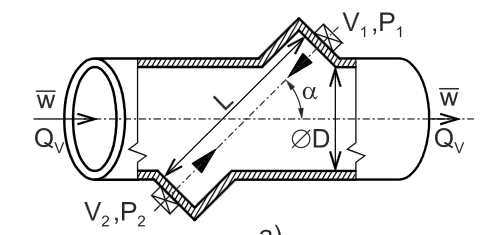
\includegraphics[width=0.4\linewidth]{figs/ultrazvukovy_prutokomer.png}
    \caption{Ultrazvukový průtokoměr}
    \label{fig:ultrazvuvkovy-prutokomer}
\end{figure}
\end{tcolorbox}

\begin{tcolorbox}[title={\stepcounter{questionnumber}\thequestionnumber. Jak se dá změřit výška hladiny v nádobě? (obrázek, popis) (66-70)}]
\textbf{Nespojité senzory hladiny:} plovákové, vibrační, optické, vodivostní, kapacitní.\\
\textbf{Spojité senzory hladiny:} tlakové, vztlakové/sílové, kapacitní, ultrazvukové, radarové.

\textbf{Tlakový princip:}
\[
p_2-p_1=\rho g h
\]
=> z rozdílu tlaků se určí výška hladiny $h$.

\textbf{Kapacitní princip:} hladina mění dielektrikum mezi elektrodami => mění se kapacita. U vodivých kapalin musí být elektroda izolovaná.

\textbf{Radar/ultrazvuk:} měří se doba letu odražené vlny od hladiny.
\begin{figure}[H]
    \centering
    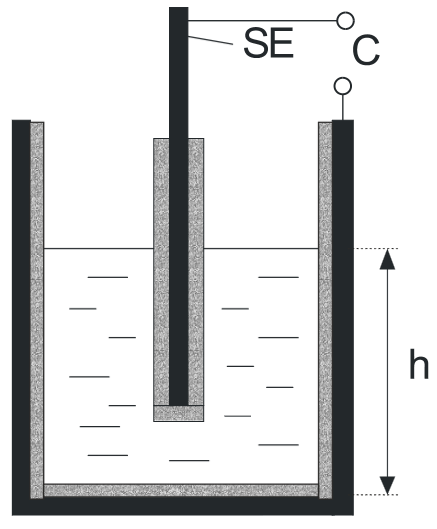
\includegraphics[width=0.15\linewidth]{figs/kapacitni_hadina.png}
    \caption{Kapacitní senzor hladiny}
    \label{fig:kapacitni-senzor-hladiny}
\end{figure}
\end{tcolorbox}

% ---------------------------------------------------------
% 11 - Chemické senzory
% ---------------------------------------------------------

\newpage
\section*{11. Chemické senzory}
\setcounter{chapternumber}{11}
\setcounter{questionnumber}{0}
% ---------------------------------------------------------

\begin{tcolorbox}[title={\stepcounter{questionnumber}\thequestionnumber. Jaké principy se používají u chemických senzorů plynů? Uveďte příklady. (3)}]
\textbf{Fyzikální princip:} změna fyzikální veličiny podle koncentrace; rychlé, ale méně selektivní. Příklady: \textbf{SAW/QMB}, tepelně vodivostní senzor, paramagnetický senzor O\textsubscript{2}.\\
\textbf{Fyzikálně-chemický princip:} chemická interakce plynu s povrchem senzoru; selektivnější, ale pomalejší. Příklady: \textbf{SnO\textsubscript{2}}, \textbf{CHEMFET}, \textbf{pellistor}.\\
\textbf{Optický princip:} plyn absorbuje elektromagnetické záření; vysoká selektivita. Příklady: \textbf{NDIR CO\textsubscript{2}}, spektrální fotometrie, photoacoustic spectroscopy.
\end{tcolorbox}

\begin{tcolorbox}[title={\stepcounter{questionnumber}\thequestionnumber. Popište bezkontaktní měření konduktivity kapaliny. Nakreslete princip a odvoďte vztah pro vyhodnocení vodivosti. (11–12)}]
\textbf{Bezkontaktní indukční konduktometr:} kapalina tvoří vodivou smyčku mezi dvěma transformátory, elektrody nejsou v kontaktu s roztokem => nejsou \textbf{polarizační jevy}.

\textbf{Vyhodnocení:} vodivost kapaliny se projeví jako vodivost $G=1/R_x$ smyčky:
\[
I_3=-\frac{U_G}{n_1n_3}G=-\frac{U_G}{n_1n_3R_x}
\]
\[
\gamma=GK
\]
kde $K$ je konstanta sondy. Nutná je \textbf{teplotní kompenzace}.
\begin{figure}[H]
    \centering
    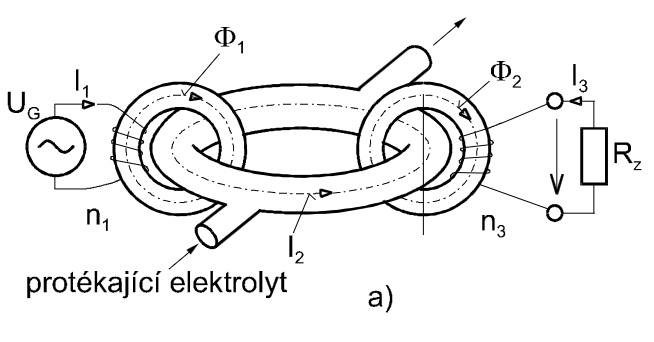
\includegraphics[width=0.5\linewidth]{figs/bezkontaktni_senzor_konduktivity.png}
    \caption{Bezkontaktní senzor konduktivity}
    \label{fig:bezkontaktni-senzor-konduktivity}
\end{figure}
\end{tcolorbox}

\begin{tcolorbox}[title={\stepcounter{questionnumber}\thequestionnumber. Nakreslete uspořádání termokatalytického senzoru – pellistoru. Popište jeho funkci a můstkové zapojení. (18)}]
\textbf{Pellistor} měří koncentraci hořlavých/výbušných plynů. Má dva vyhřívané odporové prvky:
\textbf{aktivní} s katalyzátorem a \textbf{referenční} bez katalytické reakce.

Na aktivním prvku plyn katalyticky hoří => zvýší se teplota a odpor. Oba prvky jsou ve \textbf{Wheatstoneově můstku}, takže se potlačí vliv okolní teploty.

\[
U_{\text{out}} \propto \Delta R \propto \Delta T \propto c_{\text{plynu}}.
\]
\begin{figure}[H]
    \centering
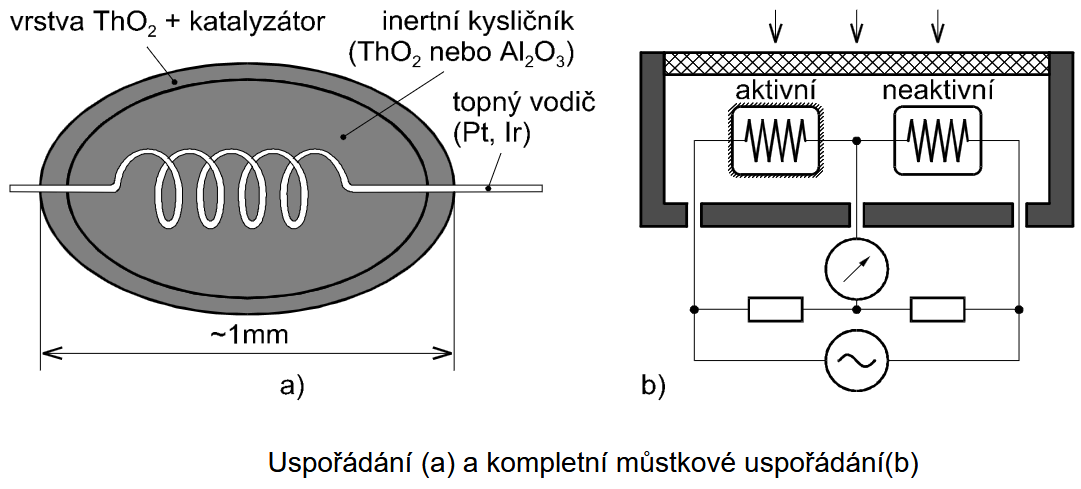
\includegraphics[width=0.75\linewidth]{figs/pelistor.png}
    \caption{Pellistor}
    \label{fig:pellistor}
\end{figure}
\end{tcolorbox}

\begin{tcolorbox}[title={\stepcounter{questionnumber}\thequestionnumber. Popište Clarkův senzor kyslíku. K čemu slouží a jaký je princip jeho funkce? (25–26)}]
\textbf{Clarkův senzor} je \textbf{amperometrický elektrochemický} senzor kyslíku. Slouží k měření koncentrace/parciálního tlaku O\textsubscript{2}.

\textbf{Princip:} membrána propouští O\textsubscript{2} do elektrolytu. Na katodě se kyslík redukuje, na anodě probíhá opačná reakce. Měřený proud je omezen difuzí kyslíku => je úměrný koncentraci O\textsubscript{2}.
\begin{figure}[H]
    \centering
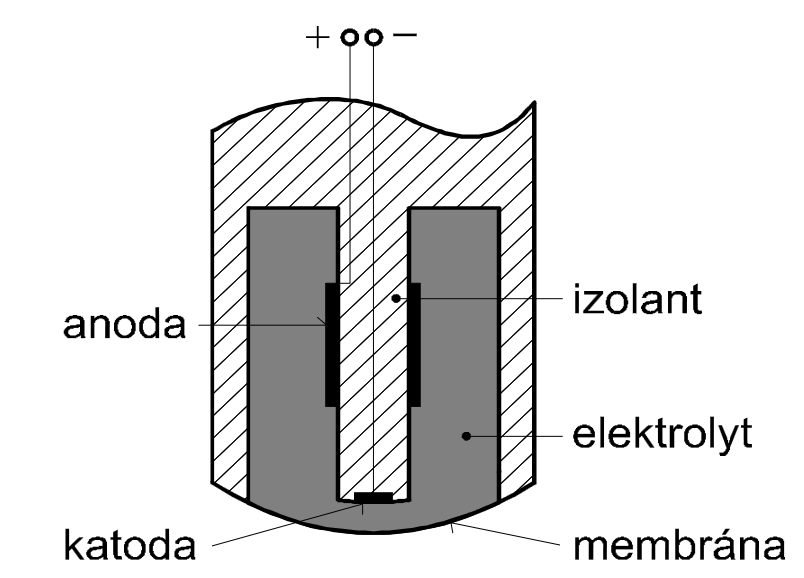
\includegraphics[width=0.25\linewidth]{figs/clarkova_elektroda.png}
    \caption{Clarkova elektroda}
    \label{fig:enter-caption-4}
\end{figure}
\end{tcolorbox}

\begin{tcolorbox}[title={\stepcounter{questionnumber}\thequestionnumber. Jaký je nejrozšířenější typ senzoru CO2? Ilustrujte na jednoduchém obrázku. (31–32)}]
\textbf{Nejrozšířenější je NDIR IR analyzátor} (Non-Dispersive Infrared). CO\textsubscript{2} absorbuje IR záření na charakteristické vlnové délce.

\textbf{Princip:} IR zdroj -> měřicí kyveta s plynem -> optický filtr -> IR detektor. Druhý kanál bývá referenční. Koncentrace se určí z útlumu podle \textbf{Lambert-Beerova zákona}:
\[
F=F_0 e^{-\varepsilon c d}
\]
\begin{figure}[H]
    \centering
    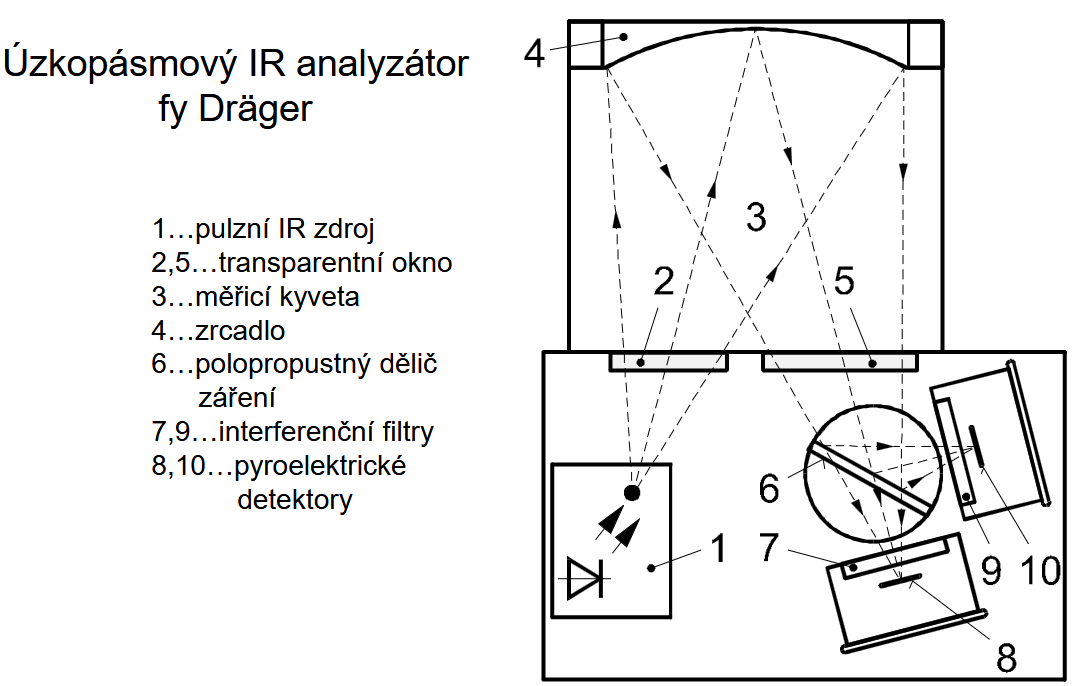
\includegraphics[width=0.75\linewidth]{figs/ir_analyzator_plynu.png}
    \caption{IR analyzátor plynu}
    \label{fig:ir-analyzator-plynu}
\end{figure}
\end{tcolorbox}

\begin{tcolorbox}[title={\stepcounter{questionnumber}\thequestionnumber. Uveďte tři principy senzorů vlhkosti vzduchu. Který je nejpřesnější? (37–47)}]
\textbf{Sorpční senzory:} hygroskopický materiál mění \textbf{odpor} nebo \textbf{kapacitu}.\\
\textbf{Psychrometr:} suchý + mokrý teploměr, z psychrometrického rozdílu se určí parciální tlak páry.\\
\textbf{Zrcadlový senzor rosného bodu:} Peltier chladí zrcadlo na právě vznikající orosení, měří se teplota rosného bodu.

\medskip
\textbf{Nejpřesnější:} \textbf{zrcadlový senzor rosného bodu}; nevýhoda = znečišťování zrcadla.
\end{tcolorbox}


\newpage
\section*{12. Etalony a další měřicí přístroje}
\setcounter{chapternumber}{12}
\setcounter{questionnumber}{0}
% ---------------------------------------------------------

\begin{tcolorbox}[title={\stepcounter{questionnumber}\thequestionnumber. Vysvětlete princip absolutního etalonu frekvence – atomových hodin. Jaké stability řádově dosahují? (4)}]
\textbf{Atomové hodiny} využívají přesně definovanou frekvenci přechodu atomu \textbf{$^{133}$Cs}.\\
\textbf{Sekunda} = 9\,192\,631\,770 period záření odpovídajícího přechodu mezi dvěma hladinami základního stavu cesia.

\textbf{Stabilita/přesnost:} malé chip-scale cca $10^{-11}$, laboratorní řádově $10^{-12}$ až $10^{-15}$.
\end{tcolorbox}

\begin{tcolorbox}[title={\stepcounter{questionnumber}\thequestionnumber. Vysvětlete princip kvantového etalonu napětí využívajícího Josephsonův jev. Jaký referenční prvek se používá v běžných napěťových referencích? (13–16)}]
\textbf{Josephsonův etalon napětí:} Josephsonův přechod ozářený elektromagnetickým polem vytvoří přesně kvantované stejnosměrné napětí:
\[
V = n \frac{h}{2e} f,
\]
kde $f$ je frekvence záření a $n$ celé číslo. Napětí je navázané na \textbf{frekvenci} a konstanty $h,e$.

\textbf{V praxi:} drahé, kryogenní technika.\\
\textbf{Běžná reference napětí:} přesná \textbf{podpovrchová Zenerova dioda}, např. LTZ1000.
\end{tcolorbox}

\begin{tcolorbox}[title={\stepcounter{questionnumber}\thequestionnumber. Vysvětlete princip kvantového etalonu odporu využívajícího kvantový Hallův jev. Jak vypadá praktický laboratorní etalon odporu? (18–20)}]
\textbf{Kvantový Hallův jev:} ve 2D elektronovém plynu při velmi nízké teplotě ($T<0{,}1$ K) a silném magnetickém poli ($B\approx18$ T) se Hallův odpor kvantuje:
\[
R_H=\frac{h}{e^2}n,\qquad R_K=\frac{h}{e^2}=25812{,}80745~\Omega
\]
kde $n$ je celé číslo nebo zlomek podle plateau. Nejistoty jsou v řádu \textbf{ppb}.

\textbf{Laboratorní etalon:} \textbf{normálový rezistor} z manganinu/podobné slitiny, mechanicky nenamáhaný, často v oleji, vždy \textbf{čtyřsvorkově}; stabilita řádově ppm.
\end{tcolorbox}

\begin{tcolorbox}[title={\stepcounter{questionnumber}\thequestionnumber. Popište základní vlastnosti laboratorního napájecího zdroje. Kdy lze zdroje spojovat sériově a proč je paralelní spojování problematické? (26–32)}]
\textbf{Laboratorní zdroj:} často vícekanálový, kanály bývají \textbf{galvanicky izolované}. Umí režim \textbf{CV} (zdroj napětí) a \textbf{CC} (zdroj proudu), má ochrany \textbf{OverVoltage/OverCurrent}.

\textbf{Sériové spojení:} možné při galvanickém oddělení; napětí se sčítají, proud omezuje nejslabší zdroj. Pozor na izolační pevnost.

\textbf{Paralelní spojení:} problém = i malý rozdíl napětí způsobí velké \textbf{vyrovnávací proudy}. Bezpečně jen u zdrojů s podporou výrobce, typicky \textbf{master-slave}.
\end{tcolorbox}

\begin{tcolorbox}[title={\stepcounter{questionnumber}\thequestionnumber. Popište základní princip spektrální analýzy pomocí FFT. Jak souvisí vzorkovací frekvence, délka FFT a frekvenční rozlišení? (33–40)}]
\textbf{FFT} převádí časový průběh do \textbf{frekvenční domény}.\\
\textbf{Vzorkovací frekvence $f_s$:} určuje rozsah spektra $0$ až $f_s/2$.\\
\textbf{Délka FFT $N$:} určuje frekvenční bin:
\[
\Delta f = \frac{f_s}{N}.
\]
Větší $N$ => lepší \textbf{frekvenční rozlišení}, ale horší \textbf{časové rozlišení}.\\
\textbf{Okénkování} (Hann, Hamming, Blackman-Harris) omezuje artefakty, když v okně není celočíselný počet period.\\
\textbf{Spektrogram/STFT:} zobrazuje změnu spektra v čase.
\end{tcolorbox}


\newpage


\newpage
\section*{Řešené příklady z poslední přednášky}
\begin{tcolorbox}[title = Příklad a)]
\begin{figure} [H]
    \centering
    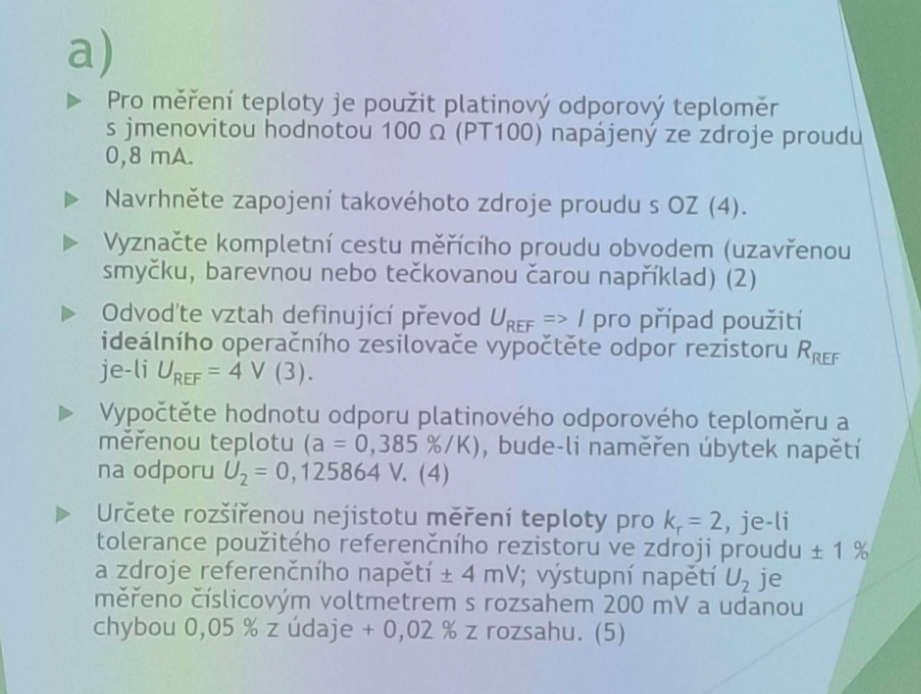
\includegraphics[width=0.5\linewidth]{figs/priklad_a_zadani.png}
    \caption{Příklad a).}
    \label{fig:priklad-a-zadani}
\end{figure}
\textbf{Řešení}: \\
\begin{figure}[H]
    \centering
    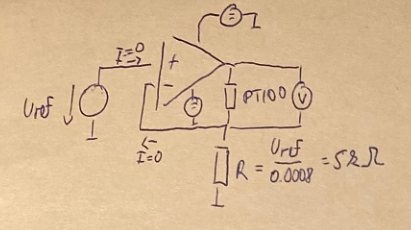
\includegraphics[width=0.5\linewidth]{figs/priklad_a_schema_reseni.png}
    \caption{Schéma řešení.}
    \label{fig:priklad-a-schema-reseni}
\end{figure}
Pokud je naměřen úbytek $U = 0.125864\ V$, znamená to, že odpor PT100 je $R= \frac{U}{I} = 157.33\ \Omega$. To odpovídá teplotě $\vartheta = \frac{157.33}{R_0\alpha} - \frac{1}{\alpha} = 148$°C.

\textbf{Nejistoty:}\\
\[u_{U_{ref}} = \frac{0.004}{\sqrt{3}}|u_R = \frac{50}{\sqrt{3}}\]
Nejistota proudu a měřeného napětí:\\
\[u_I = \sqrt{(\frac{1}{R})^2u_{U_{ref}}^2 + (-\frac{U_{ref}}{R^2})^2u_R}|u_U = \frac{\frac{0.05}{100}0.125864 + \frac{0.02}{100}0.2}{\sqrt{3}} \]
Nejistota teploty:\\
 \[\vartheta = \frac{R}{R_0\alpha} - \frac{1}{\alpha} =   \frac{U}{IR_0\alpha} - \frac{1}{\alpha}\]
 \[u_\vartheta = k_r\sqrt{(\frac{1}{IR_0\alpha})^2u_U^2 + (\frac{U^2}{IR_0\alpha})u_I^2} \]
 

 
 

\end{tcolorbox}
\begin{tcolorbox}[title = Příklad b)]
\begin{figure} [H]
    \centering
    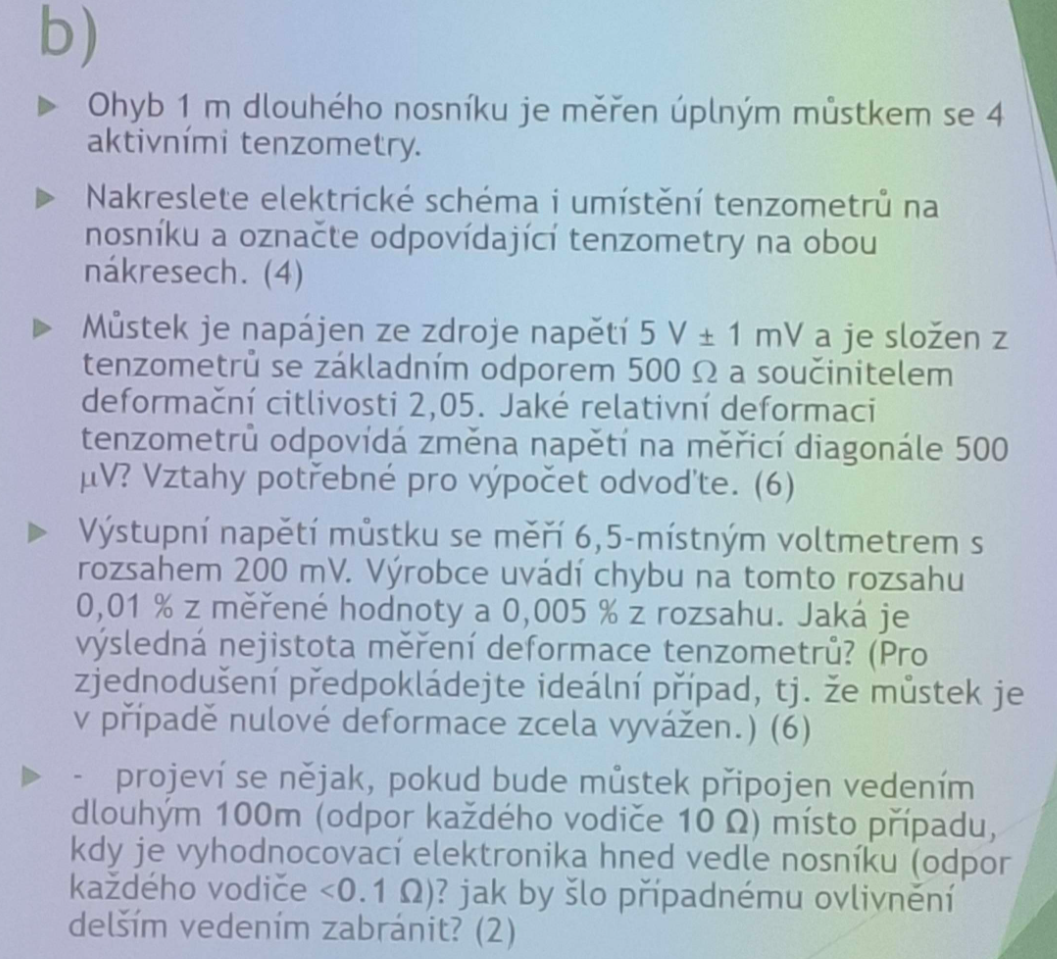
\includegraphics[width=0.5\linewidth]{figs/priklad_b_zadani.png}
    \caption{Příklad b).}
    \label{fig:priklad-b-zadani}
\end{figure}
\textbf{Řešení}: \\

\begin{figure}[H]
    \centering
    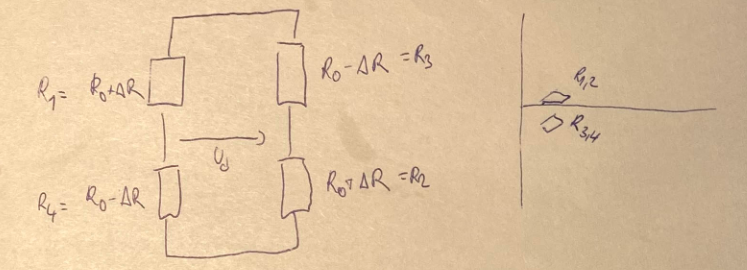
\includegraphics[width=0.5\linewidth]{figs/priklad_b_schema_reseni.png}
    \caption{Schéma řešení.}
    \label{fig:priklad-b-schema-reseni}
\end{figure}
\[2.05 = k = \frac{\frac{\Delta R}{R}}{\frac{\Delta l}{l}}|U_D = \frac{U_0\Delta R}{R}\]

Z toho vyplývá následující vztah pro relativní deformaci:
\[x = \frac{U_D}{U_0k} = 0.000048\]
\textbf{Nejistoty:}\\
\[u_{U_D} = \frac{\frac{0.01}{100}0.0005 + \frac{0.005}{100}0.2}{\sqrt{3}}|u_{U_0}=\frac{0.001}{\sqrt{3}}\]
\[u_x = \sqrt{(\frac{u_{U_D}}{U_0k})^2 + (\frac{U_Du_{U_0}}{U_0^2k})^2}\]
Odpor se přidá k každému rameni můstku, to naruší symetrii můstku a způsobí offset napětí. Lze potlačit vyhodnocováním napětí pouze na můstku - úbytek na odporu vedení se neprojeví (viz lab. 9).
\end{tcolorbox}
\begin{tcolorbox} [title = Příklad c)]
\begin{figure} [H]
    \centering
    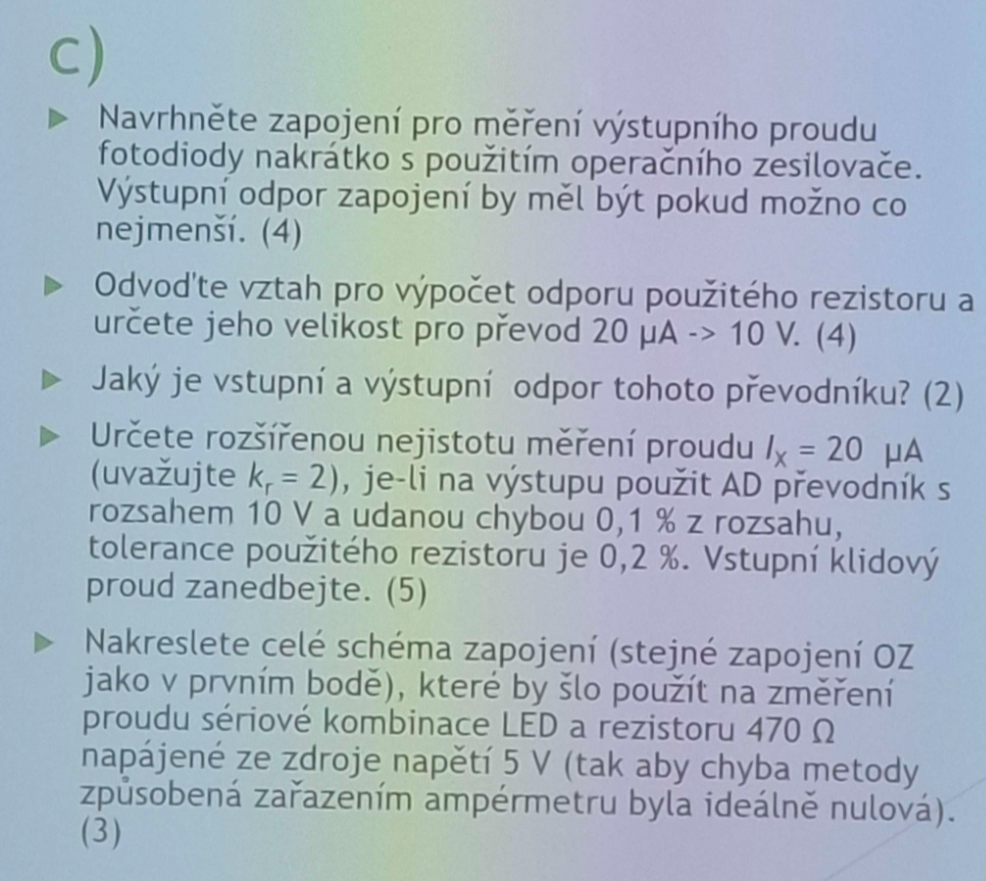
\includegraphics[width=0.5\linewidth]{figs/priklad_c_zadani.png}
    \caption{Příklad c).}
    \label{fig:priklad-c-zadani}
\end{figure}
\textbf{Řešení}: \\

\begin{figure}[H]
    \centering
    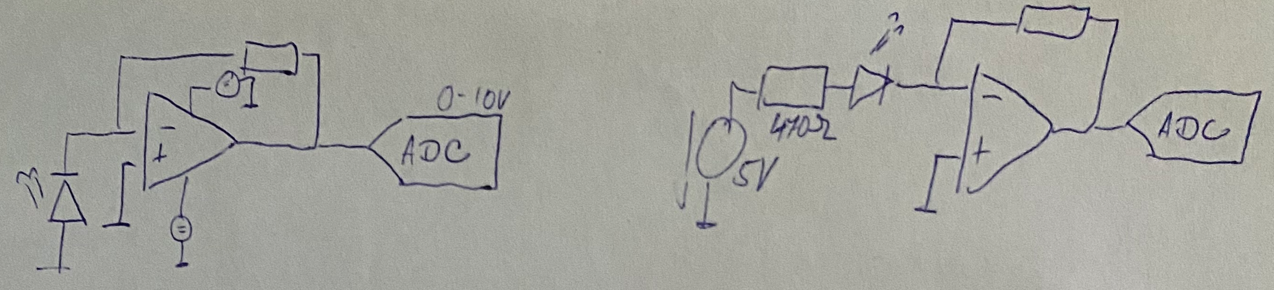
\includegraphics[width=0.5\linewidth]{figs/priklad_c_schema_reseni1.png}
    \caption{Schéma řešení.}
    \label{fig:priklad-c-schema-reseni}
\end{figure}
Pro odpor musí platit $R = \frac{U}{I} = \frac{10}{0.00002} = 500000\ \Omega$.Vstupní a výstupní odpory: $R_{in} = 0, R_{out} = 0$.
\textbf{Nejistoty:}\\
\[u_U = \frac{\frac{0.1}{100}10}{\sqrt{3}}|u_R = \frac{\frac{0.2}{100}500000}{\sqrt{3}}\]
\[u_I = k_r\sqrt{(\frac{u_U}{R})^2 + (\frac{u_RU}{R^2})^2}\]
\[I = -\frac{U_{out}}{R}\]
\end{tcolorbox}

\begin{tcolorbox}[title = Příklad d)]
    \begin{figure} [H]
        \centering
        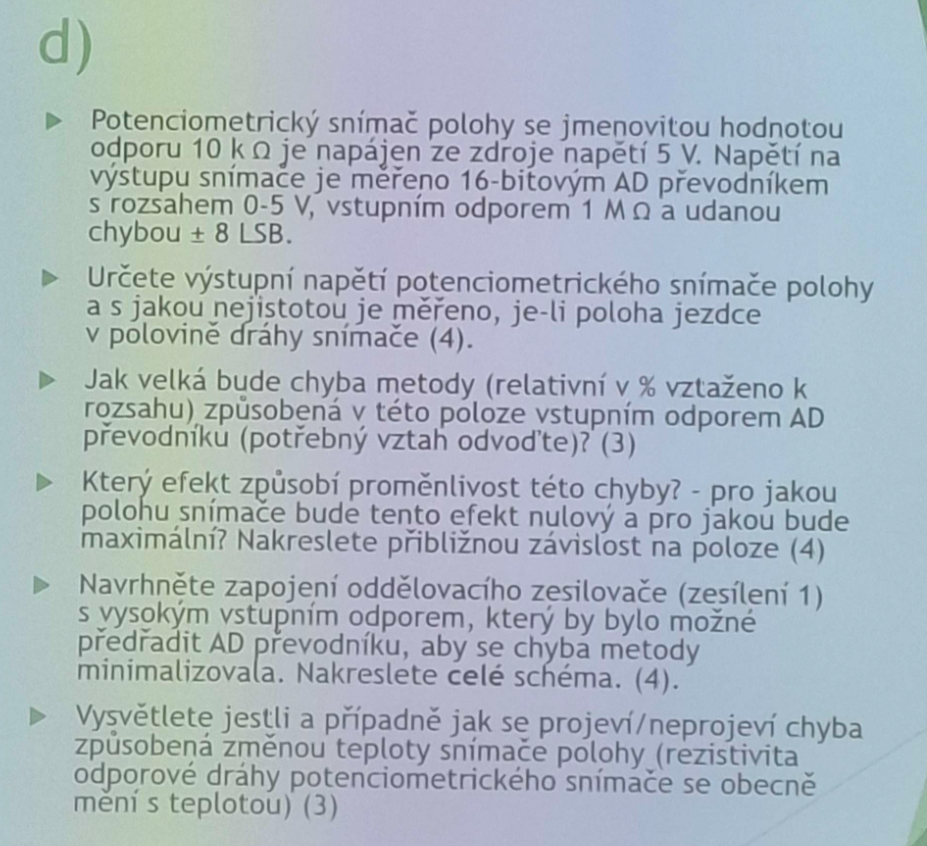
\includegraphics[width=0.5\linewidth]{figs/priklad_d_zadani.png}
        \caption{Příklad d).}
        \label{fig:priklad-d-zadani}
    \end{figure}
    \textbf{Řešení}: \\

    \begin{figure} [H]
        \centering
        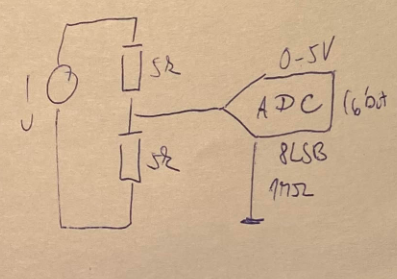
\includegraphics[width=0.5\linewidth]{figs/priklad_d_schema_reseni.png}
        \caption{Schéma řešení.}
        \label{fig:priklad-d-schema-reseni}
    \end{figure}
Nejistota je dána jako $u_U = 8 \frac{5}{2^{16}\sqrt{3}}$.\\
Výstupní odpor potenciometru je $R_{out} = 2.5\ k\Omega$
Chyba metody dána vstupním odporem ADC: \\
\[ R_{parallel} = \frac{R_{ADC}R_d}{R_{ADC} + R_d} = 4975\ \Omega\]
\[U_{mer} = U\frac{R_{parallel}}{R_{parallel}+R_{0.5}}|\delta = \frac{U_{mer}-U_{skut}}{U_{skut}}\] 
Chyba metody je největší uprostřed, nejmenší na kraji.\\
Oddělovací zesilovač - sledovač napětí.\\
Teplota snímače polohy nemá vliv u napěťového napájení a má vliv u proudového.

\end{tcolorbox}

\begin{tcolorbox} [title = Příklad e)]
\begin{figure} [H]
    \centering
    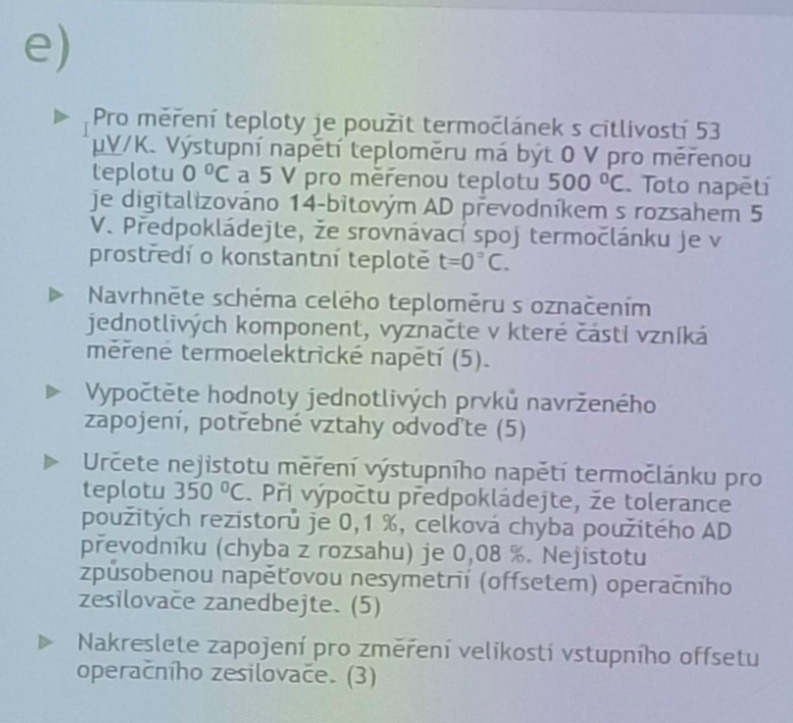
\includegraphics[width=0.5\linewidth]{figs/priklad_e_zadani.png}
    \caption{Příklad e).}
    \label{fig:priklad-e-zadani}
\end{figure}

\begin{figure}[H]
  \centering
  \begin{subfigure}{0.47\textwidth}
    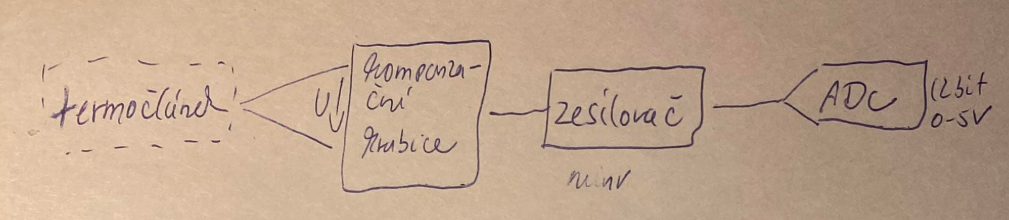
\includegraphics[width=\linewidth]{figs/priklad_e_schema_reseni.png}
    \caption{Schéma celého teploměru.}
  \end{subfigure}
  \hfill
  \begin{subfigure}{0.47\textwidth}
    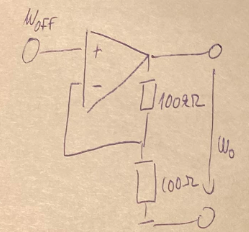
\includegraphics[width=\linewidth]{figs/priklad_e_neinvertujici_zesilovac.png}
    \caption{Zapojení pro změření velikosti $U_{off}$.}
  \end{subfigure}
  \caption{Schémata zapojení.}
  \label{fig:priklad-e-schema-reseni}
\end{figure}
Napětí $5\ V$ má odpovídat napětí na termočlánku $500\cdot0.000053\ V = 0.0265\ V$. Zesílení neinvertujícího zesilovače je $A =\frac{R_2}{R_1} + 1$, což je pro tento případ: $A = \frac{5}{0.0265} =188.67$.\\ Z toho vyplývá, že podíl rezistorů má být $\approx 187$. Nechť $R_2 = 1870\ \Omega$ a $R_1 = 10\ \Omega$.\\
\textbf{Nejistoty:}
\[u_{R_2} = 1870\frac{0.1}{100},\ u_{R_1} = 10\frac{0.1}{100},\ u_{u_0} = 5\frac{0.08}{100\sqrt{3}}\]

\[u_{u_t} = \sqrt{{(\frac{R_1}{R_1+R_2}u_{u_0}})^2 +(\frac{u_{u_0}-u_{u_0}R_1}{(R_1+R_2)^2}u_{R_1})^2 + (-\frac{u_{u_0}R_1}{(R_1+R_2)^2}u_{R_2})^2}\]


\[U_{off} = \frac{U_0}{1001}\]
\end{tcolorbox}

\begin{tcolorbox}[title = Příklad f)]
\begin{figure} [H]
    \centering
    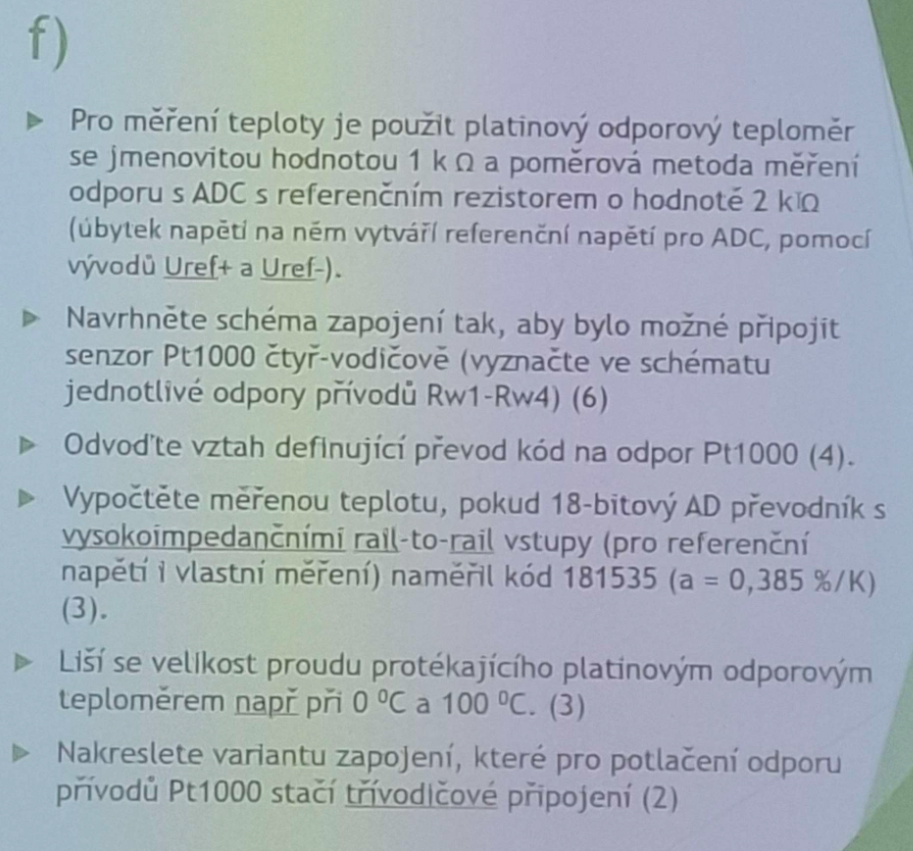
\includegraphics[width=0.5\linewidth]{figs/priklad_f_zadani.png}
    \caption{Příklad f).}
    \label{fig:priklad-f-zadani}
\end{figure}

\begin{figure}[H]
  \centering
  \begin{subfigure}{0.47\textwidth}
    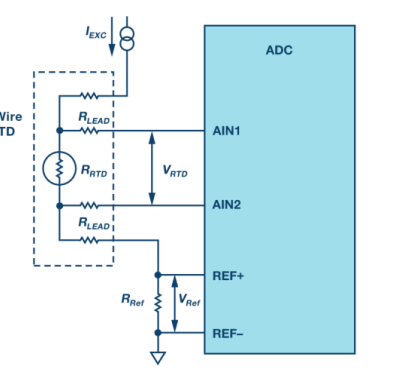
\includegraphics[width=\linewidth]{figs/priklad_f_schema_reseni.png}
    \caption{Schéma řešení.}
  \end{subfigure}
  \hfill
  \begin{subfigure}{0.47\textwidth}
    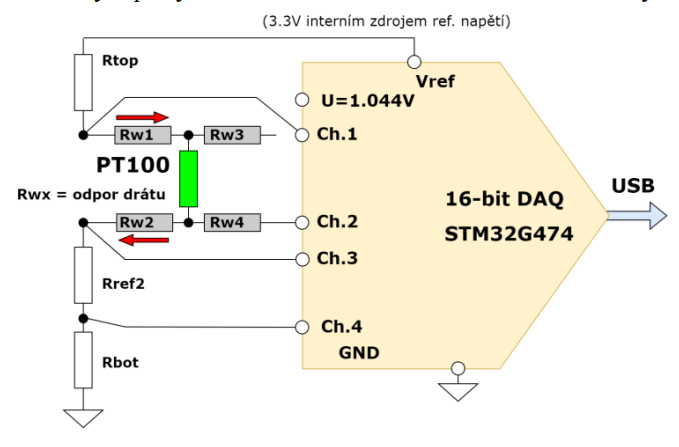
\includegraphics[width=\linewidth]{figs/priklad_f_schema2.png}
    \caption{Třívodičové zapojení.}
  \end{subfigure}
  \caption{Schémata zapojení.}
  \label{fig:priklad-f-schema-reseni}
\end{figure}


\[ U_{PT} = R_{PT}I|U_{ref} = R_{ref}I\]
\[R_{PT} = \frac{U_{PT} }{U_{ref}}R_{ref}|R_{PT} = \frac{N}{N_{max}}R_{ref}\]
\[R_{PT} = \frac{181535}{2^{18}}2000 = R_0(1+\alpha T)=2000(1+0.00385T)\]
Proud se neliší.

\end{tcolorbox}

\begin{tcolorbox}[title = Příklad g)]
Navrhněte zapojení kompenzovaného senzoru proudu pro bezdotykové měření stejnosměrného proudu (se jhem). (6).\\

Výstupní napětí převodníku je měřeno 12bitovým AČ (AD) převodníkem s rozsahem 2,5 V.\\

Vypočtěte hodnoty jednotlivých prvků navrženého zapojení tak, aby proudu $I_1$ = 25 A odpovídalo výstupní napětí $U_2$ = 2,5 V. Velikost kompenzačního proudu $I_2$ volte tak, aby výkon na odporu $R_2$, na kterém se měři výstupní napětí $U_2$, nepřevýšil 0,25 W. Kolik bude závitů kompenzačního vinuti? Potřebné vztahy odvodte (8).\\

Určete nejistotu měření proudu. Při výpočtu předpokládejte, že tolerance použitého odporů je 0,1 \%, celková chyba použitého AČ (AD) převodníku (chyba z rozsahu) je 5 LSB. Nejistotu způsobenou dalšími vlivy zanedbejte. (8)\\
\begin{figure} [H]
    \centering
    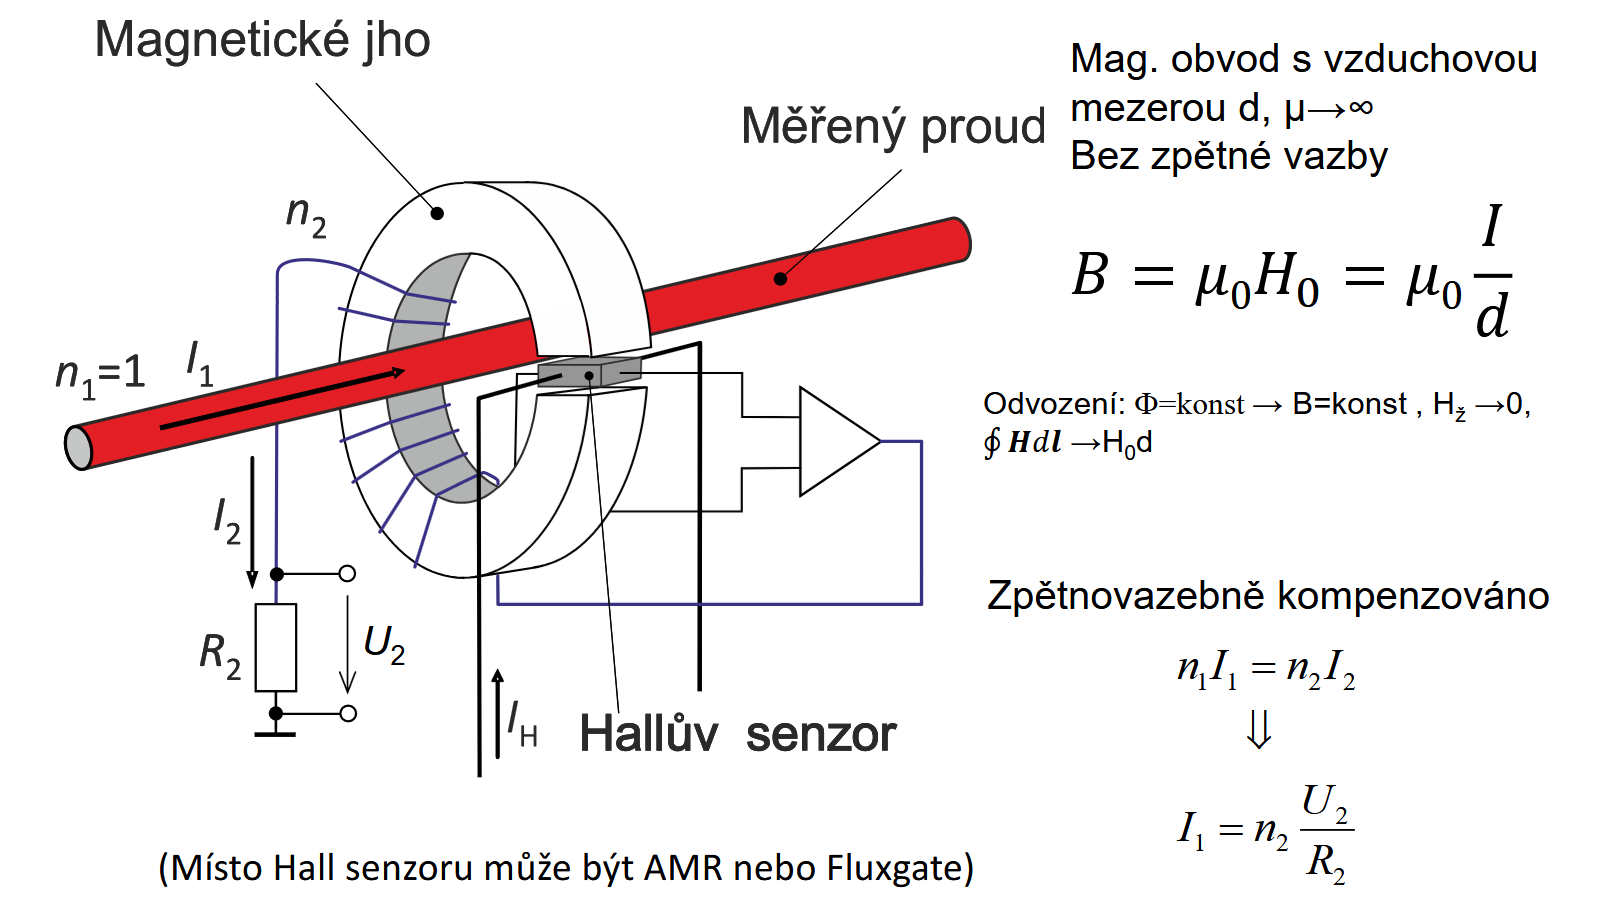
\includegraphics[width=0.5\linewidth]{figs/priklad_g_schema_reseni.png}
    \caption{Schéma řešení.}
    \label{fig:priklad-g-schema-reseni}
\end{figure}

  Aby výkon nepřekročil \(0.25\,\mathrm{W}\), musí platit: $
  R_2 \ge \frac{U_2^2}{P_{\max}}
  = \frac{2.5^2}{0.25}
  = 25\,\Omega, \text{volíme tedy }  R_2 = 25\,\Omega.
  $

  Kompenzační proud potom bude: $
  I_2 = \frac{U_2}{R_2}
  = \frac{2.5}{25}
  = 0.1\,\mathrm{A}.
  $

  Počet závitů kompenzačního vinutí: $
  N_2 = \frac{N_1 I_1}{I_2}
  = \frac{1 \cdot 25}{0.1}
  = 250.
  $
  
  \subsection*{Nejistota měření}
Chyba 5 LSB napětí $U_2$ odpovídá nejistotě $u_{U_2} = 5\frac{2.5}{2^{12}\sqrt{3}}$ a chyba odporu $R_2$ je $u_{R_2} = \frac{\frac{0.1}{100}25}{\sqrt{3}}$. \\
Celková nejistota měření tedy bude: \\  
\[u_{I_1}= \sqrt{(\frac{u_{U_2}}{R_2}n)^2+(\frac{Uu_{R_2}}{R_2^2}n)^2}\]
Relativní nejistotu dostaneme jako $\delta = \frac{u_{I_1}}{I_1}$.\\

\end{tcolorbox}

\begin{tcolorbox}[title = Příklad h)]
Navrhněte obvod pro měření střídavého proudu v rozsahu do $I_1$ = 100 $A_{RMS}$ pomocí proudového transformátoru T60404-E4626-X002 (převodový poměr 1:2500, rozsah 100 A) a AD převodníku. Máte k dispozici precizní rezistor R = 7.5 $\Omega$ (s nízkým splotním koeficientem odporu TCR), operační zesilovač s dalšími libovolnými rezistory a 16-bitový SAR AD převodník s rozsahem ±2.5V a vzorkovací rychlostí 150 kSa/s. Obvod sestavte tak, aby se rozsah AD převodníku co nejlépe využil. (16)\\

Vypočítejte nejistotu měření proudu $I_1$ = 50 A. Proudový transformátor má udanou chybu 1\% z rozsahu 100 A, AD převodník 0.1\% z rozsahu, rezistory 0.1\%. Uved'te postup výpočtu a proveďte též numerický výpočet (8)\\

  

\begin{figure} [H]
    \centering
    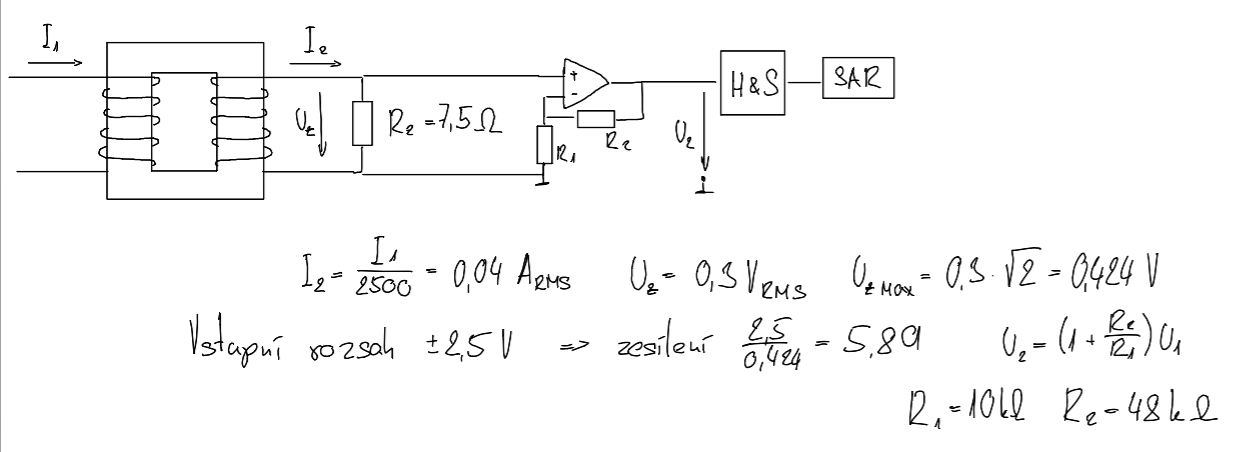
\includegraphics[width=0.8\linewidth]{figs/priklad_h_schema_reseni.png}
    \caption{Schéma řešení.}
    \label{fig:priklad-h-schema-reseni}
\end{figure}

Pro $I_1=50~A$ je $I_2=\frac{I_1}{n}=20~mA$ a na rezistoru $R=7{,}5~\Omega$ je
  $U_R=I_2R=0{,}15~V$. Po zesílení $A=5{,}8$ je výstupní napětí pro ADC
  $U_{out}=AU_R=5{,}8\cdot0{,}15=0{,}87~V$.\\

  Nejistota transformátoru:
  \[
  u_T=\frac{\frac{1}{100}\cdot100}{\sqrt{3}}=0{,}577~A
  \]

  Nejistota ADC:
  
  \[
  u_{ADC}=\frac{\frac{0{,}1}{100}\cdot2{,}5}{\sqrt{3}}=1{,}44~mV
  \]

  Nejistota rezistoru:
   \[
  u_R=\frac{\frac{0{,}1}{100}\cdot7{,}5}{\sqrt{3}}=4{,}33~m\Omega
  \]

  Celková nejistota měření:
  \[
  u_{I_1}=
  \sqrt{
  u_T^2+
  \left(\frac{n}{AR}u_{ADC}\right)^2+
  \left(\frac{U_Rn}{AR^2}u_R\right)^2
  }
  0{,}584~A
  \]

  Relativní nejistota:
  \[
  \delta=\frac{u_{I_1}}{I_1}=\frac{0{,}75}{50}= 1{,}17~\%.
  \]

\end{tcolorbox}



\end{document}
